\documentclass[a4paper,11pt]{article}

\usepackage{../../../Template/zemplate}

\usepackage{float}
\usepackage[dvipsnames]{xcolor}
\usepackage{hyperref}
%\setcounter{tocdepth}{2}

\docTitle{Manuale del manutentore}
\docVersion{2.0.0}
\docCreationDate{\frmdata{01}{04}{2017}}
\docLastUpdateDate{\frmdata{21}{08}{2017}}
\docStatus{Approvato}
\docEditors{Jordan Gottardo}
\docVerificators{Giovanni Prete}
\docApprovers{Marco Pasqualini}
\docUse{Esterno}
\docDestination{\Tullio \\ & \Cardin \\ & \zephyrus \\ & \riskapp}
\docJournal{
	2.0.0 & \frmdata{21}{08}{2017} & Marco Pasqualini & \responsabile & Approvazione documento \\
	1.1.0 & \frmdata{20}{08}{2017} & Giovanni Prete & \verificatore & Verifica documento \\
	1.0.3 & \frmdata{19}{08}{2017} & Jordan Gottardo & \programmatore & Modificata sezione 6.1 Analisi di rischio inserendo l'attuale descrizione dell'implementazione tramite mock \\
	1.0.2 & \frmdata{19}{08}{2017} & Jordan Gottardo & \programmatore & Rimossa sezione 6.1 Scenari di danno \\
	1.0.1 & \frmdata{19}{08}{2017} & Jordan Gottardo & \programmatore & Aggiunto Axios sezione 2.15  \\
	1.0.0 & \frmdata{09}{04}{2017} & Giovanni Prete & \responsabile & Approvazione documento  \\
	0.3.0 & \frmdata{08}{04}{2017} & Leonardo Brutesco & \verificatore & Verifica documento  \\	
	0.2.1 & \frmdata{06}{04}{2017} & Giulia Petenazzi & \programmatore & Correzione errori sezione 5  \\
	0.2.0 & \frmdata{05}{04}{2017} & Leonardo Brutesco & \verificatore & Verifica documento  \\
	0.1.3 & \frmdata{05}{04}{2017} & Giulia Petenazzi & \programmatore & Stesura sezione 6 - Estensione delle funzionalità e del codice e sezione 7 - Estensione del codice \\
	0.1.2 & \frmdata{04}{04}{2017} & Giovanni Damo & \programmatore & Stesura sezione 5 - Componenti \\
	0.1.1 & \frmdata{02}{04}{2017} & Giovanni Damo & \programmatore & Aggiunte versioni browser sezione 3\\	
	0.1.0 & \frmdata{02}{04}{2017} & Marco Pasqualini & \verificatore & Verifica documento \\
	0.0.2 & \frmdata{01}{04}{2017} & Giovanni Damo & \programmatore & Stesura sezioni 1 - Introduzione, 2 - Tecnologie utilizzate e 3 - Configurazione ambiente di lavoro \\
	0.0.1 & \frmdata{01}{04}{2017} & Giovanni Damo & \programmatore & Creazione template e indice\\
}
\newcommand\VRule[1][\arrayrulewidth]{\color{white} \vrule width 1pt}
\catcode`\_=12

\begin{document}
%\setcounter{secnumdepth}{2} % to block out subsubparagraph from showing out with its numbering (index etc.)

\newpage

\section{Introduzione}
	\subsection{Scopo del documento}
	Il presente documento rappresenta il Manuale del Manutentore per il progetto \progetto{} sviluppato dal gruppo \zephyrus{} per il proponente \riskapp. 
	All'interno di esso vengono descritte:
	\begin{itemize}
		\item le tecnologie utilizzate per lo sviluppo;
		\item gli strumenti utilizzati e consigliati;
		\item l'architettura del software con i relativi componenti;
		\item le funzionalità presenti.
	\end{itemize}
	Tutto ciò viene descritto per aiutare lo sviluppatore a comprendere a fondo l'applicazione per eventualmente apportarvi delle modifiche o estensioni, assumendo e richiedendo che lo sviluppatore conosca già le tecnologie utilizzate nel progetto e brevemente illustrate nella prossima sezione.
	%
	\subsection{Scopo del prodotto}
	\introScopo
	%
	\subsection{Glossario}
	Allo scopo di rendere più semplice e chiara la comprensione del manuale, nel presente documento viene incluso un breve glossario.
	Per evidenziare un termine presente in tale documento, esso verrà marcato con il pedice \textsubscript{G}. Solo la prima occorrenza del termine in ogni sezione sarà marcata per non appesantire la lettura del documento.
	Tutti i termini del glossario evidenziati sono link ipertestuali al termine corrispettivo presente nel glossario.
	%
	\subsection{Riferimenti}
	%
%		\subsubsection{Riferimenti normativi}
%		\begin{itemize}
%			\item \ndpv;
%			\item \textbf{\glo{Capitolato}{capitolato} d'appalto C3:} \href{http://www.math.unipd.it/~tullio/IS-1/2016/Progetto/C3.pdf}{http://www.math.unipd.it/~tullio/IS-1/2016/Progetto/C3.pdf};
%		\end{itemize}
		%
		\subsubsection{Riferimenti informativi}
		\begin{itemize}
			\item \textbf{Introduzione a CSS3: }
			\href{https://www.w3schools.com/css/css3_intro.asp}{https://www.w3schools.com/css/css3_intro.asp};
			\item \textbf{introduzione a HTML5:}
			\href{https://www.w3schools.com/html/html5_intro.asp}{https://www.w3schools.com/html/html5_intro.asp};
			\item \textbf{guida a ES6:}
			\href{http://es6-features.org/\#Constants}{http://es6-features.org/\#Constants};
			\item \textbf{introduzione a JSON:}
			\href{https://www.w3schools.com/js/js_json_intro.asp}{https://www.w3schools.com/js/js_json_intro.asp};
			\item \textbf{introduzione a JSX:}
			\href{https://facebook.github.io/react/docs/introducing-jsx.html}{https://facebook.github.io/react/docs/introducing-jsx.html};
			\item \textbf{Node.js:}
			\href{https://nodejs.org/it/}{https://nodejs.org/it/};
			\item \textbf{guida a OpenLayers:}
			\href{https://openlayersbook.github.io/}{https://openlayersbook.github.io/};
			\item \textbf{guida a Open Street Map:}
			\href{http://wiki.openstreetmap.org/wiki/Beginners\%27_guide}{http://wiki.openstreetmap.org/wiki/Beginners\%27_guide};
			\item \textbf{guida a React:}
			\href{https://facebook.github.io/react/}{https://facebook.github.io/react/};
			\item \textbf{React Color:}
			\href{https://casesandberg.github.io/react-color/}{https://casesandberg.github.io/react-color/};
			\item \textbf{React-Redux:}
			\href{https://github.com/reactjs/react-redux}{https://github.com/reactjs/react-redux};
			\item \textbf{React Toolbox:}
			\href{http://react-toolbox.com/#/}{http://react-toolbox.com/\#/};
			\item \textbf{Redux:}
			\href{http://redux.js.org/docs/basics/}{http://redux.js.org/docs/basics/};
			\item \textbf{SVG tutorial:}
			\href{https://www.w3schools.com/graphics/svg_intro.asp}{https://www.w3schools.com/graphics/svg_intro.asp}
		\end{itemize}
	

\newpage

\section{Tecnologie utilizzate}
In questa sezione vengono elencate le tecnologie su cui si basa lo sviluppo del progetto. Per ognuna di esse verrà indicato l'ambito di utilizzo e una descrizione.

\begin{table}[H]
	\centering
	\begin{tabular}{cl}
		\toprule
		Tecnologia & Utilizzo \\
		\midrule
		\nameref{CSS3} & Linguaggio per la formattazione delle pagine web \\
		\nameref{HTML5} & Linguaggio per la costruzione di pagine web \\
		\nameref{JavaScript ES6}  & Linguaggio principale in cui è sviluppata l'applicazione \\
		\nameref{JSON} & Formato dati utilizzato per lo scambio di informazioni \\
		\nameref{JSX} & Estensione \glo{JavaScript}{JavaScript} per l'integrazione del codice \glo{HTML}{HTML} \\
		\nameref{Node.js} & Ambiente operativo per utilizzare \js{} lato server \\
		\nameref{OpenLayers} & Libreria per la gestione della mappa e del grafo \\
		\nameref{Open Street Map} & Libreria per la fornitura di mappe in formato vettoriale \\
		\nameref{React} & Costruzione dell'interfaccia grafica \\
		\nameref{ReactColor} & Libreria per gestire la palette di colori \\
		\nameref{React-Redux} & libreria per interfacciare \glo{React}{React} con Redux \\ 
		\nameref{React Toolbox} & Libreria che implementa la specifica di Material Design \\
		\nameref{Redux}  & Libreria per l'implementazione dell'architettura \\
		\nameref{SVG} & Scalable Vector Graphics \\
		
		\bottomrule
	\end{tabular}
	\caption{Tabella riassuntiva tecnologie utilizzate nel progetto}
\end{table}

\subsection{CSS3}
\label{CSS3}
\begin{table}[H]
	\centering
	\begin{tabular}{p{2cm}p{0.5cm}p{11.5cm}}
		\arrayrulecolor{lightgray}
		\toprule
		\textbf{Descrizione} & &
		È un linguaggio utilizzato per la presentazione di documenti HTML. Lo standard viene definito dal \glo{W3C}{W3C}.
		\\ \midrule
		\textbf{Utilizzo} & &
		Viene utilizzato per definire il layout dell'applicazione.
		\\ \midrule
		\textbf{Documentazione ufficiale} & &
		\url{https://www.w3schools.com/css/css3_intro.asp}
		\\ \bottomrule
	\end{tabular}
\end{table}

\vspace{40px}
\subsection{HTML5}
\label{HTML5}
\begin{table}[H]
	\centering
	\begin{tabular}{p{2cm}p{0.5cm}p{11.5cm}}
		\arrayrulecolor{lightgray}
		\toprule
		\textbf{Descrizione} & &
		È un \glo{Linguaggio di markup}{linguaggio di markup} utilizzato per definire la struttura delle pagine web. Lo standard viene definito dal W3C.
		\\ \midrule
		\textbf{Utilizzo} & &
		Viene utilizzato per definire il layout dell'applicazione.
		\\ \midrule
		\textbf{Documentazione ufficiale} & &
		\url{https://www.w3.org/TR/html5/}
		\\ \bottomrule
	\end{tabular}
\end{table}

\vspace{40px}
\subsection{JavaScript ES6}
\label{JavaScript ES6}
\begin{table}[H]
	\centering
	\begin{tabular}{p{2cm}p{0.5cm}p{11.5cm}}
		\arrayrulecolor{lightgray}
		\toprule
		\textbf{Descrizione} & &
		\js{} è un linguaggio di scripting orientato agli oggetti e agli eventi, utilizzato principalmente nella programmazione Web lato client.
		Le caratteristiche più importanti di questo linguaggio sono:
		\begin{itemize}
			\item \textbf{eventi:} quando l'utente interagisce con la pagina Web in vari modi, come ad esempio mouse e tastiera, viene generato un evento; \js{} gestisce  tali eventi, i quali possono avviare un'azione registrata in un gestore di eventi;
			\item \textbf{tipizzazione dinamica:} il programmatore non è tenuto a specificare il tipo degli oggetto che utilizza;
			\item \textbf{paradigma a protipi:} stile di programmazione orientato ad oggetti in cui l'ereditarietà è implementata tramite il riuso di oggetti esistenti, basandosi sul loro prototipo.
		\end{itemize}
		In particolare, il \glo{Gruppo}{gruppo} si baserà sull'utilizzo della specifica \jsv{}, che definisce significativi cambiamenti sintattici per la scrittura di applicazioni complesse in modo più semplice.
		\\ \midrule
		\textbf{Utilizzo} & &
		\js{} è il linguaggio base con cui si svilupperà l'applicazione \progetto{}. Di conseguenza è ance il linguaggio utilizzato maggiormente dalle librerie esterne da noi sfruttate.
		\\ \midrule
		\textbf{Documentazione ufficiale} & &
		\url{http://www.ecma-international.org/ecma-262/6.0/}
		\\ \bottomrule
	\end{tabular}
\end{table}

\vspace{40px}
\subsection{JSON}
\label{JSON}
\begin{table}[H]
	\centering
	\begin{tabular}{p{2cm}p{0.5cm}p{11.5cm}}
		\arrayrulecolor{lightgray}
		\toprule
		\textbf{Descrizione} & &
		Formato dati utilizzato per lo scambio di informazioni tra il client (ovvero il nostro prodotto) e il server (ovvero il prodotto di \riskapp).
		\\ \midrule
		\textbf{Utilizzo} & &
		Viene utilizzato per lo scambio di dati tra l'applicazione \progetto e il server di \riskapp.
		\\ \midrule
		\textbf{Documentazione ufficiale} & &
		\url{http://www.json.org}
		\\ \bottomrule
	\end{tabular}
\end{table}

\vspace{40px}
\subsection{JSX}
\label{JSX}
\begin{table}[H]
	\centering
	\begin{tabular}{p{2cm}p{0.5cm}p{11.5cm}}
		\arrayrulecolor{lightgray}
		\toprule
		\textbf{Descrizione} & &
		JSX è un linguaggio orientato agli oggetti staticamente tipizzato. È un'estensione di \js.
		I file in linguaggio JSX vengono poi tradotti in \js.
		\\ \midrule
		\textbf{Utilizzo} & &
		Viene utilizzato come sintassi all'interno di React.
		\\ \midrule
		\textbf{Documentazione ufficiale} & &
		\url{https://facebook.github.io/react/docs/introducing-jsx.html}
		\\ \bottomrule
	\end{tabular}
\end{table}

\vspace{40px}
\subsection{Node.js}
\label{Node.js}
\begin{table}[H]
	\centering
	\begin{tabular}{p{2cm}p{0.5cm}p{11.5cm}}
		\arrayrulecolor{lightgray}
		\toprule
		\textbf{Descrizione} & &
		Ambiente operativo per utilizzare \js{} in ambito server.
		\\ \midrule
		\textbf{Utilizzo} & &
		Viene utilizzato per far avviare la nostra applicazione.
		\\ \midrule
		\textbf{Documentazione ufficiale} & &
		\url{https://nodejs.org/it/docs/}
		\\ \midrule
		\textbf{Versione installata} & &
		6.9.1
		\\ \bottomrule
	\end{tabular}
\end{table}

\vspace{40px}
\subsection{OpenLayers}
\label{OpenLayers}
\begin{table}[H]
	\centering
	\begin{tabular}{p{2cm}p{0.5cm}p{11.5cm}}
		\arrayrulecolor{lightgray}
		\toprule
		\textbf{Descrizione} & &
		E' una libreria \js{} per visualizzare mappe interattive nei browser web.
		OpenLayers offre \glo{API}{API} ai programmatori per poter accedere a diverse fonti d'informazioni cartografiche in Internet: mappe del progetto OpenStreetMap, mappe sotto licenze non-libere (Google Maps, Bing, Yahoo), Web Feature Service, ecc. E' coperto da licenza BSD.
		\\ \midrule
		\textbf{Utilizzo} & &
		Viene utilizzato per gestire la mappa.
		\\ \midrule
		\textbf{Documentazione ufficiale} & &
		\url{http://openlayers.org/en/latest/doc/}
		\\ \midrule
		\textbf{Versione installata} & &
		4.0.1
		\\ \bottomrule
	\end{tabular}
\end{table}

\vspace{40px}
\subsection{Open Street Map}
\label{Open Street Map}
\begin{table}[H]
	\centering
	\begin{tabular}{p{2cm}p{0.5cm}p{11.5cm}}
		\arrayrulecolor{lightgray}
		\toprule
		\textbf{Descrizione} & &
		E' una libreria \js{} per fornire informazioni geografiche in formato vettoriale.
		\\ \midrule
		\textbf{Utilizzo} & &
		OpenStreetMap viene utilizzato in modo indiretto dalla libreria OpenLayers per fornire una vista
		vettoriale nella mappa dell'applicazione.
		\\ \midrule
		\textbf{Documentazione ufficiale} & &
		\url{https://www.openstreetmap.org/help}
		\\\bottomrule
	\end{tabular}
\end{table}

\vspace{40px}
\subsection{React}
\label{React}
\begin{table}[H]
	\centering
	\begin{tabular}{p{2cm}p{0.5cm}p{11.5cm}}
		\arrayrulecolor{lightgray}
		\toprule
		\textbf{Descrizione} & &
		E' una libreria \js{} \glo{Open source}{open source} mantenuta da Facebook e Instagram utile alla costruzione di interfacce grafiche. Per fare ciò, React utilizza componenti indipendenti e riusabili che ereditano dalla classe base astratta React.Component. Le componenti devono implementare il metodo \glo{Render}{render}() che si occupa di rappresentare la \glo{Componente}{componente} sul browser.
		Le caratteristiche più importanti di questa libreria sono:
		\begin{itemize}
			\item {\textbf{One-way-data-flow:}} meccanismo tramite il quale le proprietà (un insieme di valori immutabili passato al render di un componente) non possono essere direttamente modificate. Queste proprietà possono però essere modificate da una \glo{Callback}{callback};
			\item {\textbf{Virtual DOM:}} virtualizzazione operata da React per effettuare un re-rendering efficiente dei componenti. 
			Consiste in:
			\begin{itemize}
				\item replicare il DOM in memoria;
				\item individuare le differenze tra il DOM reale e il DOM virtuale;
				\item aggiornare le informazioni del DOM reale sulla base delle differenze precedentemente individuate.
			\end{itemize}
			\item utilizzo di JSX.
		\end{itemize}
		\\ \midrule
		\textbf{Utilizzo} & &
		React viene utilizzata per la costruzione dell'interfaccia grafica dell'applicazione.
		\\ \midrule
		\textbf{Documentazione ufficiale} & &
		\url{https://facebook.github.io/react/docs/hello-world.html}
		\\ \midrule
		\textbf{Versione installata} & &
		15.4.2
		\\ \bottomrule
	\end{tabular}
\end{table}

\vspace{40px}
\subsection{ReactColor}
\label{ReactColor}
\begin{table}[H]
	\centering
	\begin{tabular}{p{2cm}p{0.5cm}p{11.5cm}}
		\arrayrulecolor{lightgray}
		\toprule
		\textbf{Descrizione} & &
		E' una libreria \js{} per creare una palette di colori RGB.
		\\ \midrule
		\textbf{Utilizzo} & &
		Viene  utilizzata per la creazione di un color picker.
		\\ \midrule
		\textbf{Documentazione ufficiale} & &
		\url{https://casesandberg.github.io/react-color/}
		\\ \midrule
		\textbf{Versione installata} & &
		2.11.3
		\\ \bottomrule
	\end{tabular}
\end{table}

\vspace{40px}
\subsection{React-Redux}
\label{React-Redux}
\begin{table}[H]
	\centering
	\begin{tabular}{p{2cm}p{0.5cm}p{11.5cm}}
		\arrayrulecolor{lightgray}
		\toprule
		\textbf{Descrizione} & &
		Libreria che facilita l'integrazione tra Redux e React.
		\\ \midrule
		\textbf{Utilizzo} & &
		Le classi \js{} vengono passate ad una funzione della libreria per ottenere una nuova classe che sfrutti React-Redux.
		\\ \midrule
		\textbf{Documentazione ufficiale} & &
		\url{http://redux.js.org/docs/basics/UsageWithReact.html}
		\\ \midrule
		\textbf{Versione installata} & &
		5.0.3
		\\ \bottomrule
	\end{tabular}
\end{table}

\vspace{40px}
\subsection{React Toolbox}
\label{React Toolbox}
\begin{table}[H]
	\centering
	\begin{tabular}{p{2cm}p{0.5cm}p{11.5cm}}
		\arrayrulecolor{lightgray}
		\toprule
		\textbf{Descrizione} & &
		E' una libreria \js{} composta da un insieme di componenti React che implementano la specifica del Material Design di Google.
		\\ \midrule
		\textbf{Utilizzo} & &
		React Toolbox viene utilizzata per implementare alcune le componenti grafiche secondo la specifica del Material Design.
		\\ \midrule
		\textbf{Documentazione ufficiale} & &
		\url{http://react-toolbox.com/#/components}
		\\ \midrule
		\textbf{Versione installata} & &
		2.0.0-beta.7
		\\\bottomrule
	\end{tabular}
\end{table}

\vspace{40px}
\subsection{Redux}
\label{Redux}
\begin{table}[H]
	\centering
	\begin{tabular}{p{2cm}p{0.5cm}p{11.5cm}}
		\arrayrulecolor{lightgray}
		\toprule
		\textbf{Descrizione} & &
		Libreria per l’implementazione dell’architettura che si occupa di gestire le interazioni tra la business logic e la presentazione.
		Per fare ciò:
		\begin{itemize}
			\item implementa un \glo{Design pattern}{design pattern} architetturale da usare il sostituzione a MVC, come descritto in
			\nameref{dp_redux};
			\item offre delle API apposite per la gestione degli elementi del design pattern descritto al punto precedente.
		\end{itemize}
		\\ \midrule
		\textbf{Utilizzo} & &
		Redux viene utilizzato per implentare l'archiettura di \progetto.
		\\ \midrule
		\textbf{Documentazione ufficiale} & &
		\url{http://redux.js.org}
		\\ \midrule
		\textbf{Versione installata} & &
		3.6.0
		\\\bottomrule
	\end{tabular}
\end{table}

\vspace{40px}
\subsection{SVG}
\label{SVG}
\begin{table}[H]
	\centering
	\begin{tabular}{p{2cm}p{0.5cm}p{11.5cm}}
		\arrayrulecolor{lightgray}
		\toprule
		\textbf{Descrizione} & &
		Standard per la scrittura di immagini in formato vettoriale.
		\\ \midrule
		\textbf{Utilizzo} & &
		SVG viene utilizzato per aggiungere oggetti personalizzati alla mappa.
		\\ \midrule
		\textbf{Documentazione ufficiale} & &
		\url{https://www.w3.org/Graphics/SVG/}
		\\ \midrule
		\textbf{Versione installata} & &
		0.1.0
		\\\bottomrule
	\end{tabular}
\end{table}

\vspace{40px}
\subsection{Axios}
\label{Axios}
\begin{table}[H]
	\centering
	\begin{tabular}{p{2cm}p{0.5cm}p{11.5cm}}
		\arrayrulecolor{lightgray}
		\toprule
		\textbf{Descrizione} & &
		Libreria JavaScript per la gestione di richieste HTTP.
		\\ \midrule
		\textbf{Utilizzo} & &
		Viene utilizzato per effettuare le chiamate verso il server di Riskapp.
		\\ \midrule
		\textbf{Documentazione ufficiale} & &
		\url{https://github.com/mzabriskie/axios}
		\\ \midrule
		\textbf{Versione installata} & &
		0.16.2
		\\\bottomrule
	\end{tabular}
\end{table}
\newpage

\section{Configurazione ambiente di lavoro}
In questa sezione verranno descritti gli strumenti utilizzati e consigliati per lo sviluppo dell'applicazione. Inoltre verranno descritte delle procedure per l'installazione e la configurazione degli stessi.
%
	\subsection{Requisiti di sistema}
	Essendo \progetto{} un'applicazione web, è necessaria una connessione ad internet per poterla utilizzare.
	\subsubsection{Dispositivi e browser supportati}
		Al momento della stesura di questo documento l'applicazione è supportata dai seguenti dispositivi:
		\begin{itemize}
			\item Window v10
			\item Linux Ubuntu10.04 e Debian 8.0
			\item MacOS v10.2
			\item Tablet - Asus P01MA con sistema operativo Android 6.0.1
			\item Tablet - iPad Air 2 con sistema operativo iOS 10.2
		\end{itemize}
		e dai seguenti browser:
		\begin{itemize}
			\item Chome v55
			\item Safari v10
			\item Firefox v5.3 per iOS 10.2
			\item Firefox v50
		\end{itemize}
	%
	\subsection{IDE: WebStorm}
	WebStormG è un IDE fornito dall'azienda JetBrains per lo sviluppo di applicazioni e siti web. Questo software permette di supportare lo sviluppatore nella realizzazione di prodotti web. Tra le principali funzionalità sono presenti:
	\begin{itemize}
		\item assistenza nella codifica dei principali framework web;
		\item auto-completamento per la sintassi di molti linguaggi (es. \js, HTML, CSS);
		\item gestione di progetti complessi;
		\item integrazione con i più popolari tool per lo sviluppo web;
		\item integrazione di un sistema di debugging per il codice \js;
		\item compatibilità con sistemi di build automatico.
	\end{itemize}
	Questo strumento è stato utilizzato durante l'attività di codifica e le principali motivazioni che hanno portato il gruppo alla sua scelta sono:
	\begin{itemize}
		\item strumento completo e professionale;
		\item licenza gratuita per studenti;
		\item integrabilità con strumenti per analisi statica e test;
		\item integrabilità con GitHub;
		\item cross-platform.
	\end{itemize}
	%
	\begin{table}[H]
		\centering
		\begin{tabular}{p{2cm}p{0.5cm}p{11.5cm}}
			\arrayrulecolor{lightgray}
			\toprule
			\textbf{Indirizzo download} & &
			\url{https://www.jetbrains.com/webstorm/download/}
			\\ \midrule
			\textbf{Versione installata} & &
			2017.1 o superiore
			\\ \bottomrule
		\end{tabular}
	\end{table}
	%
	\subsection{Gestore dei pacchetti}
		\subsubsection{Node.js} \label{nodejs}
		Node.js è una piattaforma event-driven per il motore \js{} V8, disponibile sulle principali piattaforme, anche se maggiormente performante su sistemi operativi UNIX-like.
		\begin{table}[H]
			\centering
			\begin{tabular}{p{2cm}p{0.5cm}p{11.5cm}}
				\arrayrulecolor{lightgray}
				\toprule
				\textbf{Indirizzo download} & &
				\url{https://nodejs.org/en/download/}
				\\ \midrule
				\textbf{Versione installata} & &
				6.9.5 o superiore
				\\ \bottomrule
			\end{tabular}
		\end{table}
		Consigliamo la versione stabile (LTS) di Node.js e non quella con le ultime features. Inoltre per verificare la versione attualmente installata, eseguire il seguente comando a terminale:
		\begin{center}
			\hicode{node -v}
		\end{center}
		%
		\subsubsection{npm} \label{npm}
		npm (node package manager) è il gestore di pacchetti di default utilizzato da Node.js. Questo strumento consente  l'installazione e la gestione di moduli esterni che forniscono funzionalità aggiuntive al sistema node di base, risolvendo varie dipendenze.
		Le principali motivazioni che hanno portato il gruppo alla scelta di questo strumento sono:
		\begin{itemize}
			\item larga diffusione;
			\item più di 400.000 pacchetti installabili;
			\item ampia documentazione.
		\end{itemize}
		\begin{table}[H]
			\centering
			\begin{tabular}{p{2cm}p{0.5cm}p{11.5cm}}
				\arrayrulecolor{lightgray}
				\toprule
				\textbf{Indirizzo download} & &
				\url{https://www.npmjs.com}
				\\ \midrule
				\textbf{Versione installata} & &
				4.2.0 o superiore
				\\ \bottomrule
			\end{tabular}
		\end{table}
		Per lo sviluppo di questo progetto è stato creato e configurato un apposito file che richiama l'installazione di tutti i pacchetti necessari. Di seguito viene descritta la procedura per l'installazione di quest'ultimo:
		\begin{enumerate}
			\item aver installato Node.js, oppure installarlo seguendo le istruzioni descritte in \ref{nodejs};
			\item aprire un terminale e posizionarsi all'interno della cartella del progetto, in modo da scaricare i pacchetti localmente . Se non presente, scaricarla tramite la procedura descritta nella sezione \ref{downloadProgetto};
			\item scrivere il comando 
			\begin{center}
				\hicode{npm install} \label{npminstall}
			\end{center}
			\item attendere il termine dell'installazione, che può durare anche qualche minuto in funzione della banda o della potenza del processore;
		\end{enumerate}
		Per vedere la lista dei pacchetti installati e controllarne la versione scrivere nel terminale all'interno della cartella del progetto \progetto:
		\begin{center}
			\hicode{npm list}
		\end{center}
	%
	\subsection{Browser}
		\subsubsection{Google Chrome}
		L'indirizzo per il download è valido per i seguenti sistemi operativi: Windows 10/8.1/8/7 64/32-bit, Mac OS X 10.9+, Linux
		\begin{table}[H]
			\centering
			\begin{tabular}{p{2cm}p{0.5cm}p{11.5cm}}
				\arrayrulecolor{lightgray}
				\toprule
				\textbf{Indirizzo download} & &
				\url{https://www.google.it/chrome/browser/desktop/index.html}
				\\ \midrule
				\textbf{Versione installata} & &
				55 o superiore
				\\ \bottomrule
			\end{tabular}
		\end{table}
		\subsubsection{Mozilla Firefox}
				L'indirizzo per il download è valido per i seguenti sistemi operativi: Windows 10/8.1/8/7 64/32-bit, Mac OS X 10.9+, Linux
		\begin{table}[H]
			\centering
			\begin{tabular}{p{2cm}p{0.5cm}p{11.5cm}}
				\arrayrulecolor{lightgray}
				\toprule
				\textbf{Indirizzo download} & &
				\url{https://www.mozilla.org/it/firefox/new/?scene=2}
				\\ \midrule
				\textbf{Versione installata} & &
				50 o superiore
				\\ \bottomrule
			\end{tabular}
		\end{table}
		\subsubsection{Safari}
		\begin{table}[H]
			\centering
			\begin{tabular}{p{2cm}p{0.5cm}p{11.5cm}}
				\arrayrulecolor{lightgray}
				\toprule
				\textbf{Indirizzo download} & &
				\url{Integrato nei Mac}
				\\ \midrule
				\textbf{Versione installata} & &
				10 o superiore
				\\ \bottomrule
			\end{tabular}
		\end{table}
	%
	\subsection{Download del progetto} \label{downloadProgetto}
	Il progetto è attualmente ospitato presso una repository privata su GitHub e quindi necessita l'autorizzazione da parte del grippo \zephyrus. Una volta ottenuta, si può procedere con la procedura seguente:
	\begin{enumerate}
		\item scaricare il progetto tramite il seguente link:
			\begin{center}
				\url{https://github.com/JordanGottardo/DeGeOP}
			\end{center}
			\begin{figure}[H]
				\centering 
				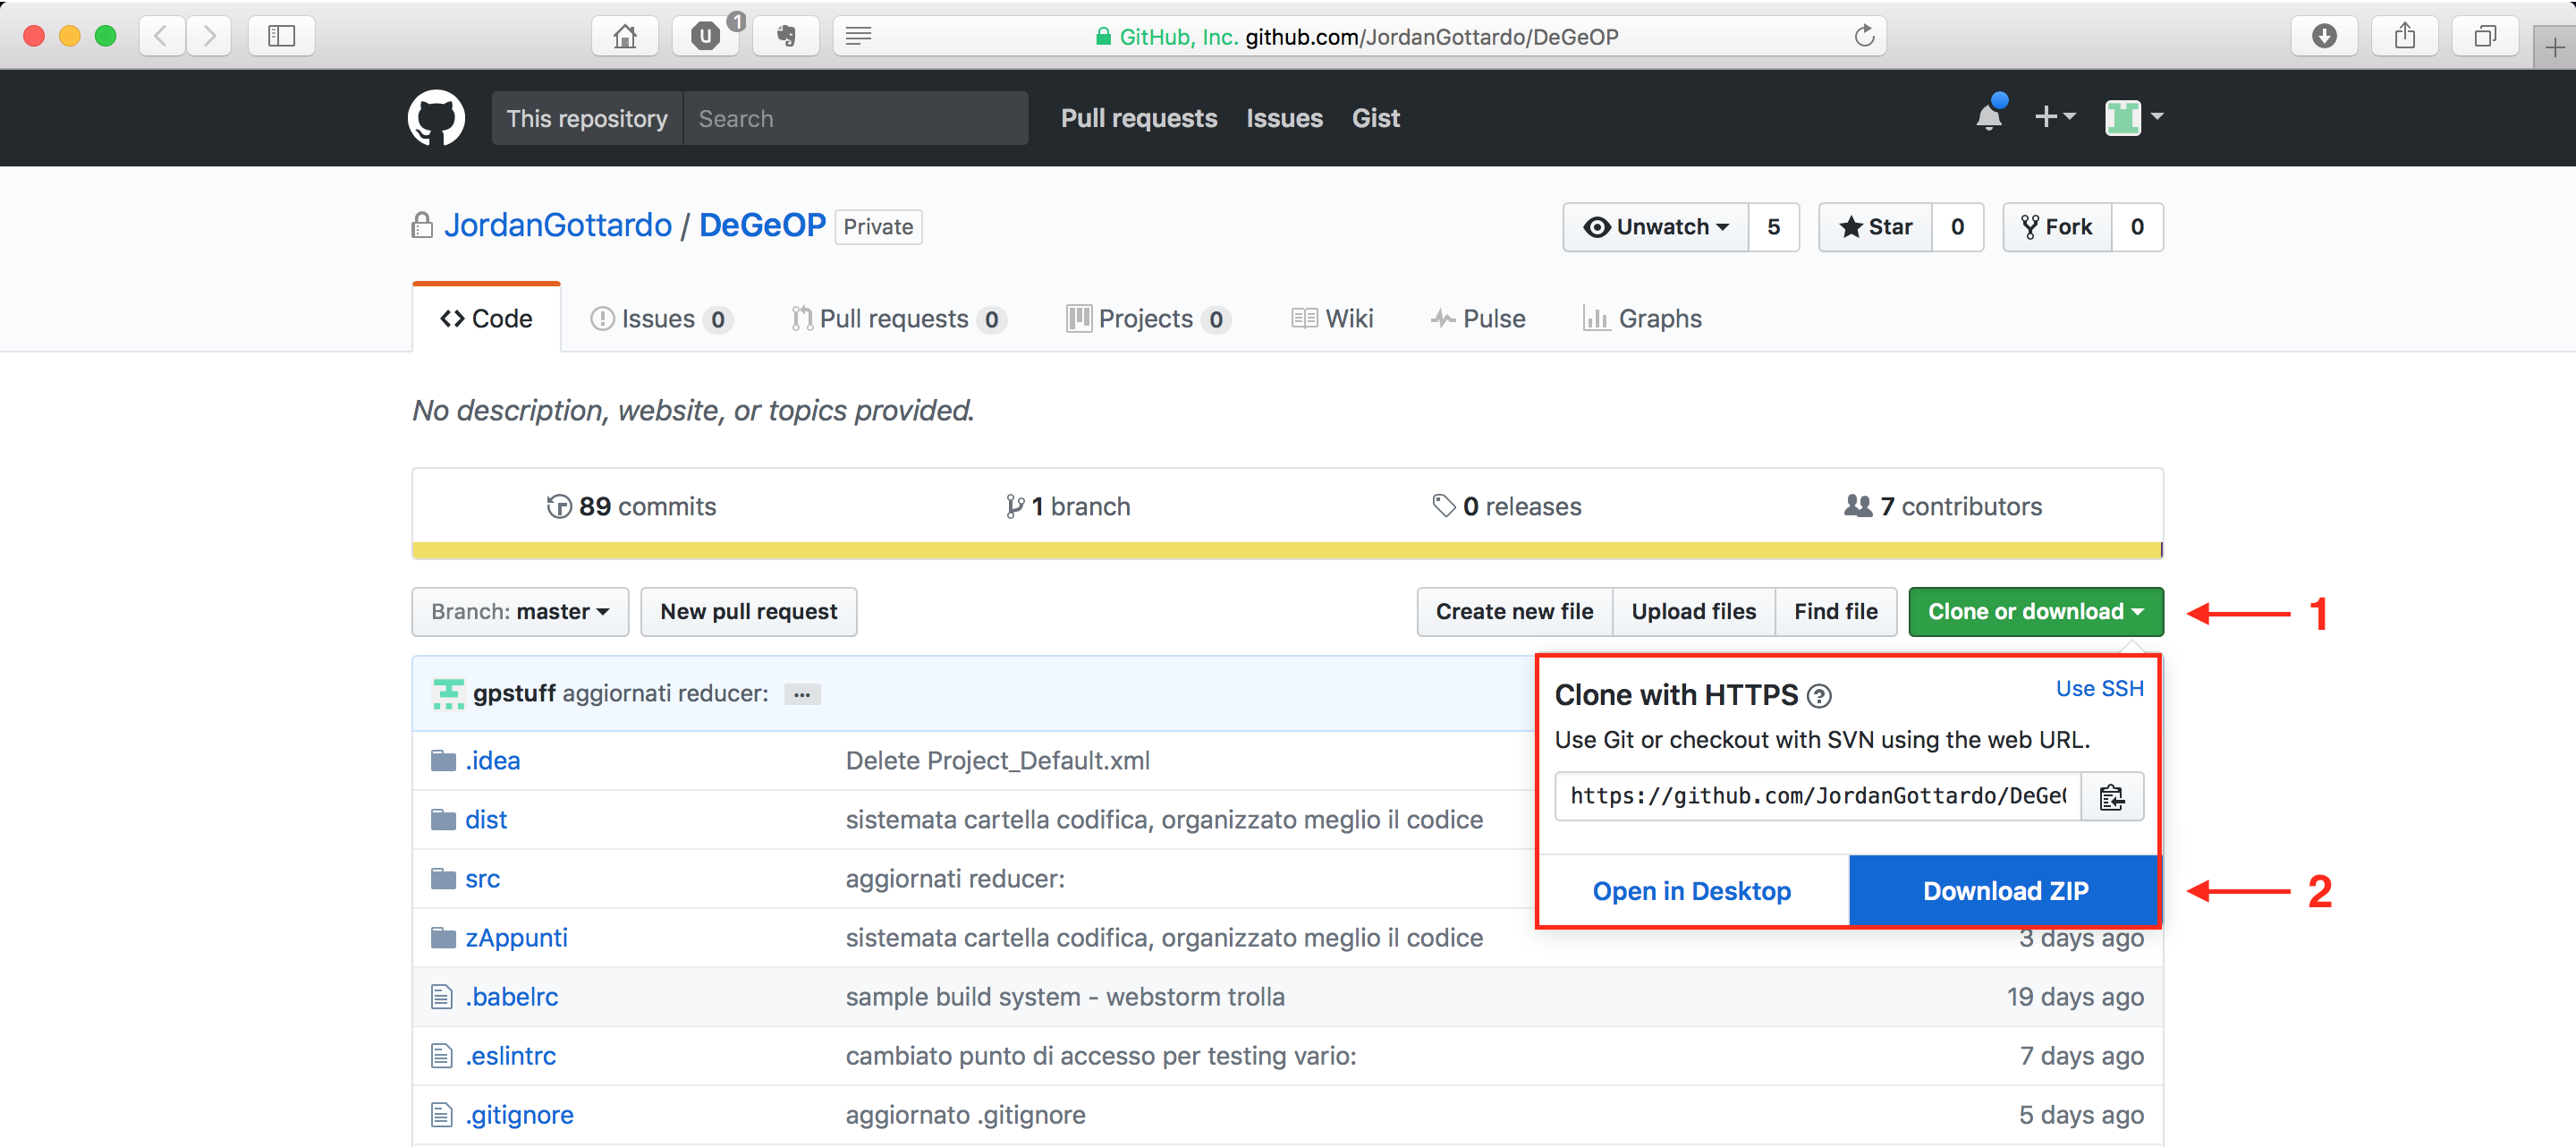
\includegraphics[width=1\columnwidth]{img/downloadProgetto.png}
				\caption{Download progetto \progetto dalla repository su GitHub}
			\end{figure}
		\item decomprimere il file \texttt{.zip} scaricato;
		\item avviare WebStorm e aprire il progetto, seguendo il menu: \hicode{File -> Open} e selezionare la cartella estratta al punto 2;
		\item (opzionale) dopo aver installato tutti i pacchetti con procedura \ref{npminstall}, è possibile configurare ESLint. Di seguito vengono descritti i passi per la configurazione su WebStorm:
			\begin{enumerate}
				\item aprire WebStorm;
				\item aprire il menu \hicode{File -> Preferences};
				\item entrare nel menu \hicode{Language \& Frameworks->JavaScript->Code Quality->ESLint};
				\item abilitare il tool essicurandosi di aver installato prima Node.js (vedi sezione \ref{nodejs});
				\item selezionare nel campo ESLint package il file che si trova all'interno del progetto \texttt{DeGeOp/node_modules/eslint};
			\end{enumerate}
			\begin{figure}[H]
				\centering 
				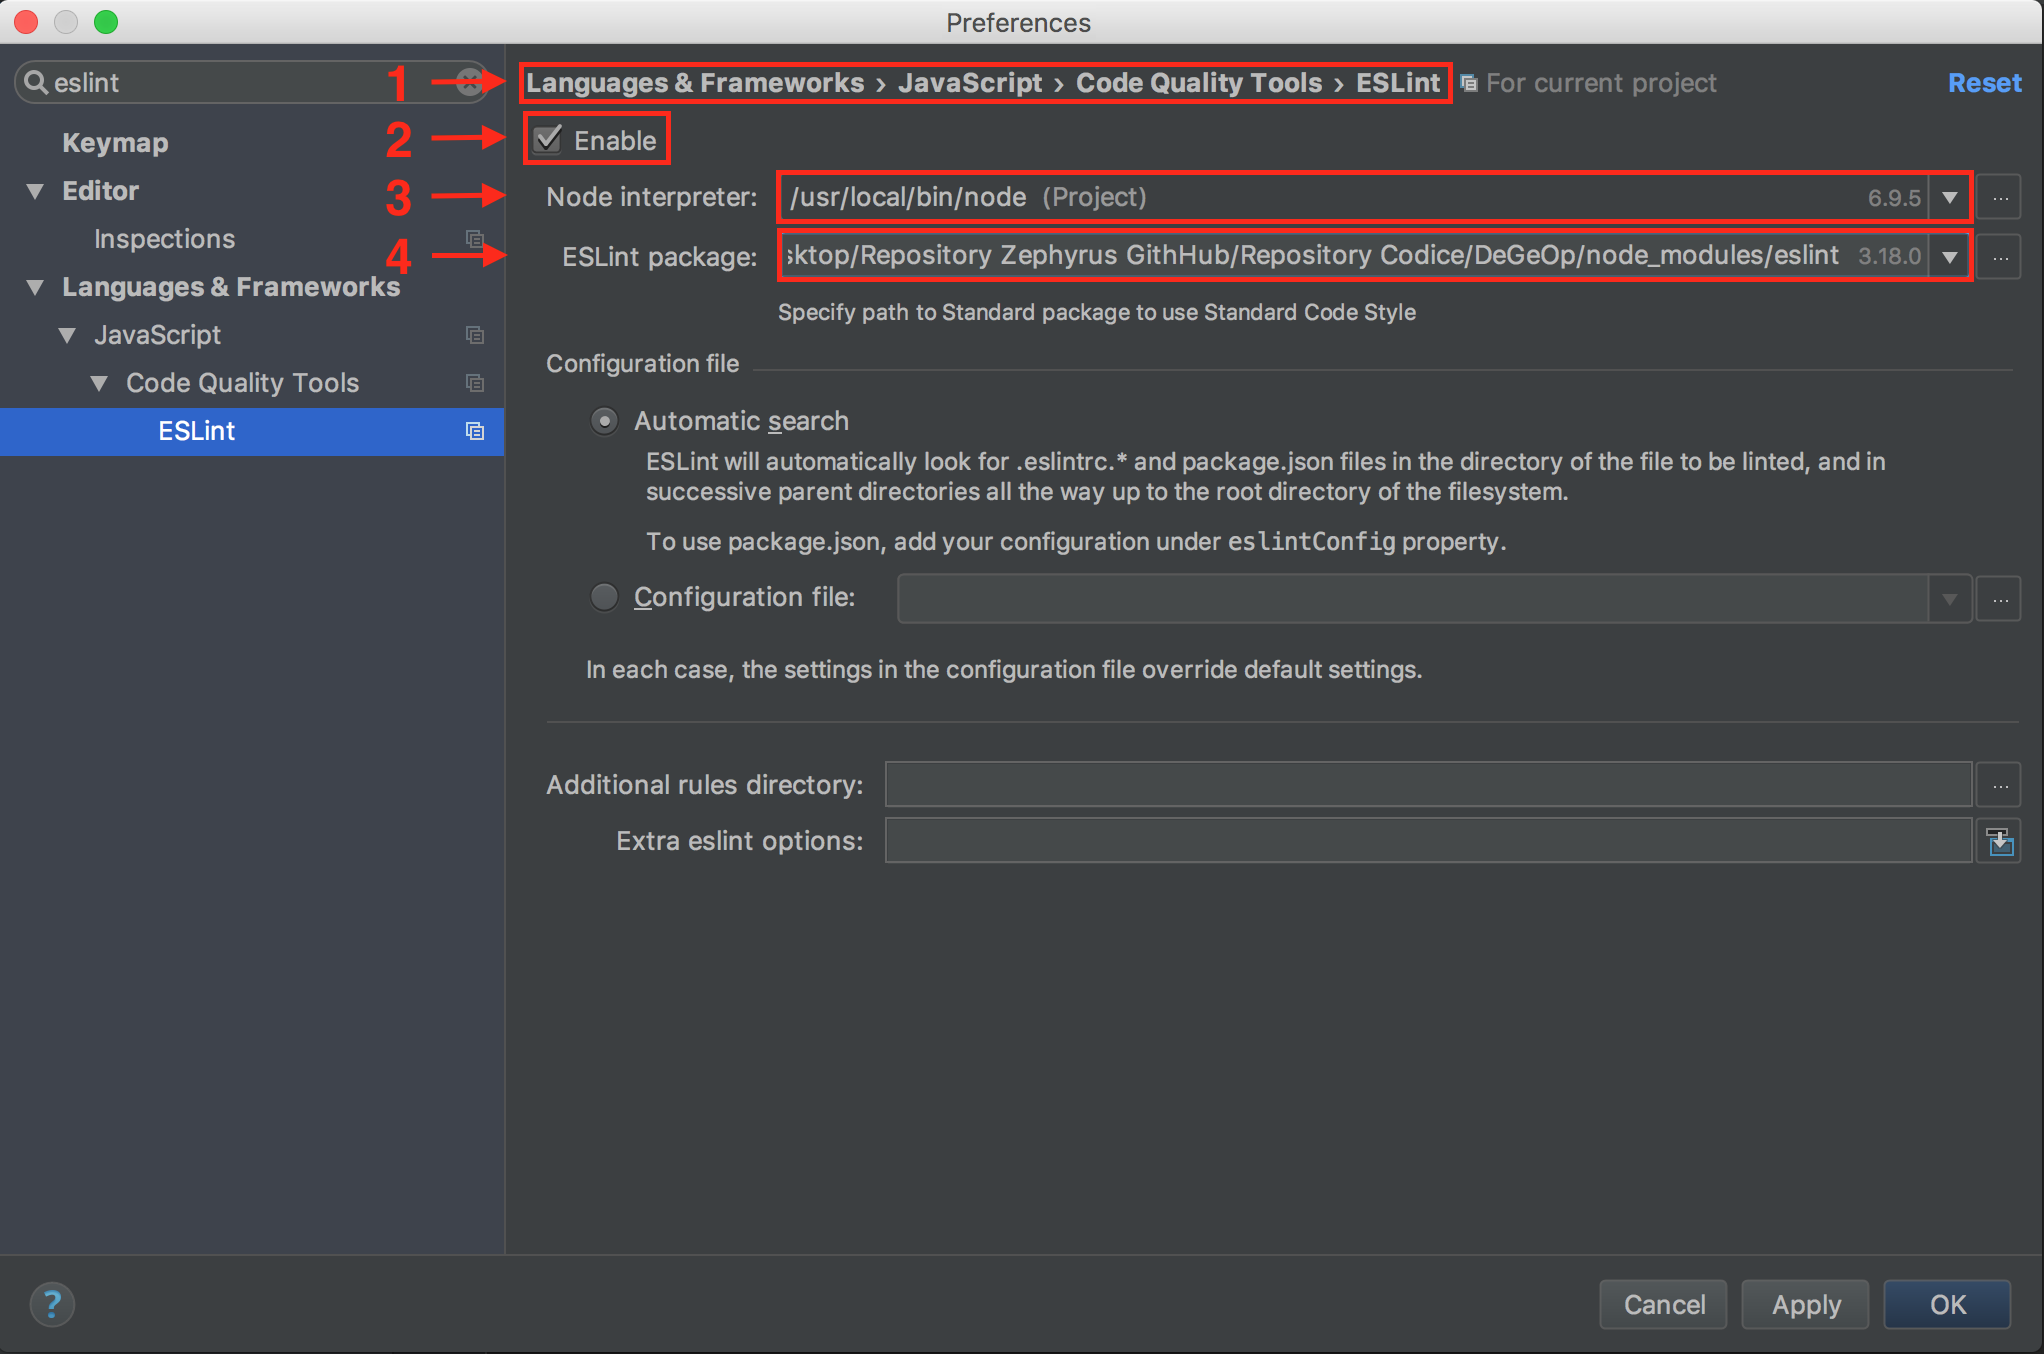
\includegraphics[width=1\columnwidth]{img/configESLint.png}
				\caption{Configurazione ESLint \progetto su WebStorm}
			\end{figure}
	\end{enumerate}
	
	%
	\subsection{Configurazione della VirtualBox}
	In accordo con il proponente abbiamo installato una macchina virtuale per effettuare il deploy e testare la nostra applicazione con il server di \riskapp{}. La procedura per configurare la macchina virtuale è la seguente:
	\begin{enumerate}
		\item scaricare e installare sul proprio computer Oracle VirtualBox dal sito ufficiale:
		\begin{center}
			\url{https://www.virtualbox.org/wiki/Downloads}
		\end{center} 
		\item scaricare il file immagine della macchina virtuale creata da \riskapp{},  dal seguente link, inserendo le apposite credenziali fornite dal proponente:
		\begin{center}
			\url{https://www.satellite1.info/u/Zephyrus.ova};
		\end{center} 
		\item aprire l'applicazione VirtualBox sul proprio computer;
		\item aprire il menù \hicode{File} e selezionare \hicode{Import Appliance};
		\item selezionare il file \hicode{Zephyrus.ova} scaricato nel punto 2 e cliccare su \hicode{Next};
		\item cliccare su \hicode{Import} e attendere la fine del processo;
		\item terminata l'importazione fare click destro sulla nuova macchina virtuale presente nell'elenco a sinistra e selezionare \hicode{Settings};
		\item selezionare la sezione \hicode{Network};
		\item nella tab \hicode{Adapter 1} modificare l'opzione \hicode{Attached to:} in \hicode{NAT} e cliccare \hicode{OK};
		\item la macchina virtuale è ora pronta all'uso.
	\end{enumerate}
	%
\newpage

\section{Architettura \progetto}
	\subsection{Introduzione}
	Il prodotto \progetto{}, creato dal \glo{Gruppo}{gruppo} \zephyrus{}, sarà integrabile nell'attuale applicazione del proponente \riskapp{}.\\
	Per esporre l'architettura dell'applicazione si procederà con approccio top-down, partendo cioè da una visione generale delle componenti che distinguono il sistema, per poi analizzare in dettaglio la conformazione di tali componenti.\\
	Il sistema attuale di \riskapp{} presenta un'architettura client-server.
	\subsection{Server}
	\progetto{} si connetterà al server di \riskapp{} esclusivamente utilizzando le \glo{API}{API} REST fornite dal proponente stesso e riportate in questa sezione. Il gruppo non ha quindi accesso all'implementazione del server di \riskapp{}.
	\subsubsection{Chiamate REST}
	L'interfaccia REST proposta da \riskapp{} fornisce l'accesso alle seguente entità:
	\begin{itemize}
		\item Customer
		\item Graph
		\item \glo{Asset}{Asset}
		\item Node
		\item Edge
	\end{itemize}
	Per ognuna di queste è possibile fare una chiamata REST usando i verbi http. (GET, OPTION, POST, PUT, UPDATE, DELETE)\\\\
	Tutte queste entità sono identificate univocamente da uno uuid formato come una stringa di cifre esadecimali con la seguente struttura:
	\begin{center}
		XXXXXXXX-XXXX-XXXX-XXXX-XXXXXXXXXXXX
	\end{center}
	Il verbo OPTION viene utilizzato all'interno del server di Riskapp per ottenere informazioni sulla struttura (nomi dei campi dati e relativi tipi di dato) delle entità ricevute a seguito di una chiamata GET o necessarie per le chiamate POST e PUT.
	Inoltre per determinati campi, la chiamata OPTION restituisce tutti i possibili valori, nel caso siano limitati al lato server, per il campo stesso.
	
	\paragraph{Customer}
	\begin{itemize}
		\item \textbf{descrizione:} l'entità customer contiene le informazioni del cliente;
		\item \textbf{chiamata:} /mitsuko/v01/customer/<uuid>/uuid/
		\begin{itemize}\item \textbf{operazioni utilizzate:} GET.\end{itemize}
	\end{itemize}
	
	\paragraph{Graph}
	\begin{itemize}
		\item \textbf{descrizione:} l'entità grafo proposta da \riskapp{} contiene le informazioni relative al processo produttivo e ai suoi \glo{Nodo}{nodi};
		\item \textbf{chiamata:} /mitsuko/v01/graph/<uuid>/uuid/
		\begin{itemize}\item \textbf{operazioni utilizzate:} GET.\end{itemize}
	\end{itemize}
	
	\paragraph{Asset}
	\begin{itemize}
		\item \textbf{descrizione:} l'entità asset rappresenta un asset del cliente con le relative informazioni;
		\item \textbf{chiamata:} /mitsuko/v01/customer/<uuid>/asset/new/
		\begin{itemize}\item \textbf{operazioni utilizzate:} POST.\end{itemize}
		\item \textbf{chiamata:} /mitsuko/v01/asset/<uuid>/uuid/
		\begin{itemize}\item \textbf{operazioni utilizzate:} GET, PUT, OPTIONS, UPDATE, DELETE.\end{itemize}
	\end{itemize}
	
	\paragraph{Node}
	\begin{itemize}
		\item \textbf{descrizione:} l'entità node rappresenta un elemento di interesse strategico all'interno di un asset;
		\item \textbf{chiamata:} /mitsuko/v01/graph/<uuid>/node/new/
		\begin{itemize}\item \textbf{operazioni utilizzate:} POST.\end{itemize}
		\item \textbf{chiamata:} /mitsuko/v01/node/<uuid>/uuid/
		\begin{itemize}\item \textbf{operazioni utilizzate:} GET, PUT, OPTIONS, UPDATE, DELETE.\end{itemize}
	\end{itemize}
	
	\paragraph{Edge}
	\begin{itemize}
		\item \textbf{descrizione:} l'entità edge rappresenta un collegamento fra due nodi;
		\item \textbf{chiamata:} /mitsuko/v01/graph/<uuid>/edge/new/
		\begin{itemize}\item \textbf{operazioni utilizzate:} POST.\end{itemize}
		\item \textbf{chiamata:} /mitsuko/v01/edge/<uuid>/uuid/
		\begin{itemize}\item \textbf{operazioni utilizzate:} GET, PUT, OPTIONS, UPDATE, DELETE.\end{itemize}
	\end{itemize}
	
	\newpage
	\subsection{Client}
	Il proponente ha fornito l'ambiente di sviluppo contenente la loro attuale applicazione, denominata in figura come "\riskapp", su cui il gruppo potrà integrare \progetto. Il prodotto sarà sviluppato come una single-page accessibile cliccando sulla scheda di menu "Process and analysis".
	
	\subsubsection{Design architetturale di DeGeOP}
	E' stato scelto di utilizzare il design architetturale Redux (per maggiori informazioni su questo pattern, si veda l'appendice \ref{dp_redux}).
	Per una migliore gestione e uso di questo pattern si è deciso di rafforzare l'uso classico di Redux, incapsulando le varie componenti in una struttura a classi.
	Rispetto all'architettura base, ovvero Redux, sono quindi presenti altre componenti:
	\begin{itemize}
		\item \textbf{ActionCreators:} struttura il cui compito è creare le "azioni", ossia le operazioni che si occupano di interagire con lo \glo{Store}{store}. Le actions come fornite da Redux permettono di definire azioni potenzialmente invalide o la cui esecuzione potrebbe portare ad errori. È quindi nata la necessità di incapsulare il concetto di azione e devolvere il compito della sua creazione ad una \glo{Componente}{componente} propria;
		\item \textbf{\glo{Reducer}{Reducer}:} classe di utilità che accetta \glo{Action}{action} generiche e le reindirizza alle giuste implementazioni per gestire l'azione in analisi. Anche in questo caso l'incapsulazione è stata adottata per fornire una migliore interfaccia di utilizzo dei reducer.
	\end{itemize}
	
	\begin{figure}[H]
		\label{diagramma_architettura}
		\centering
		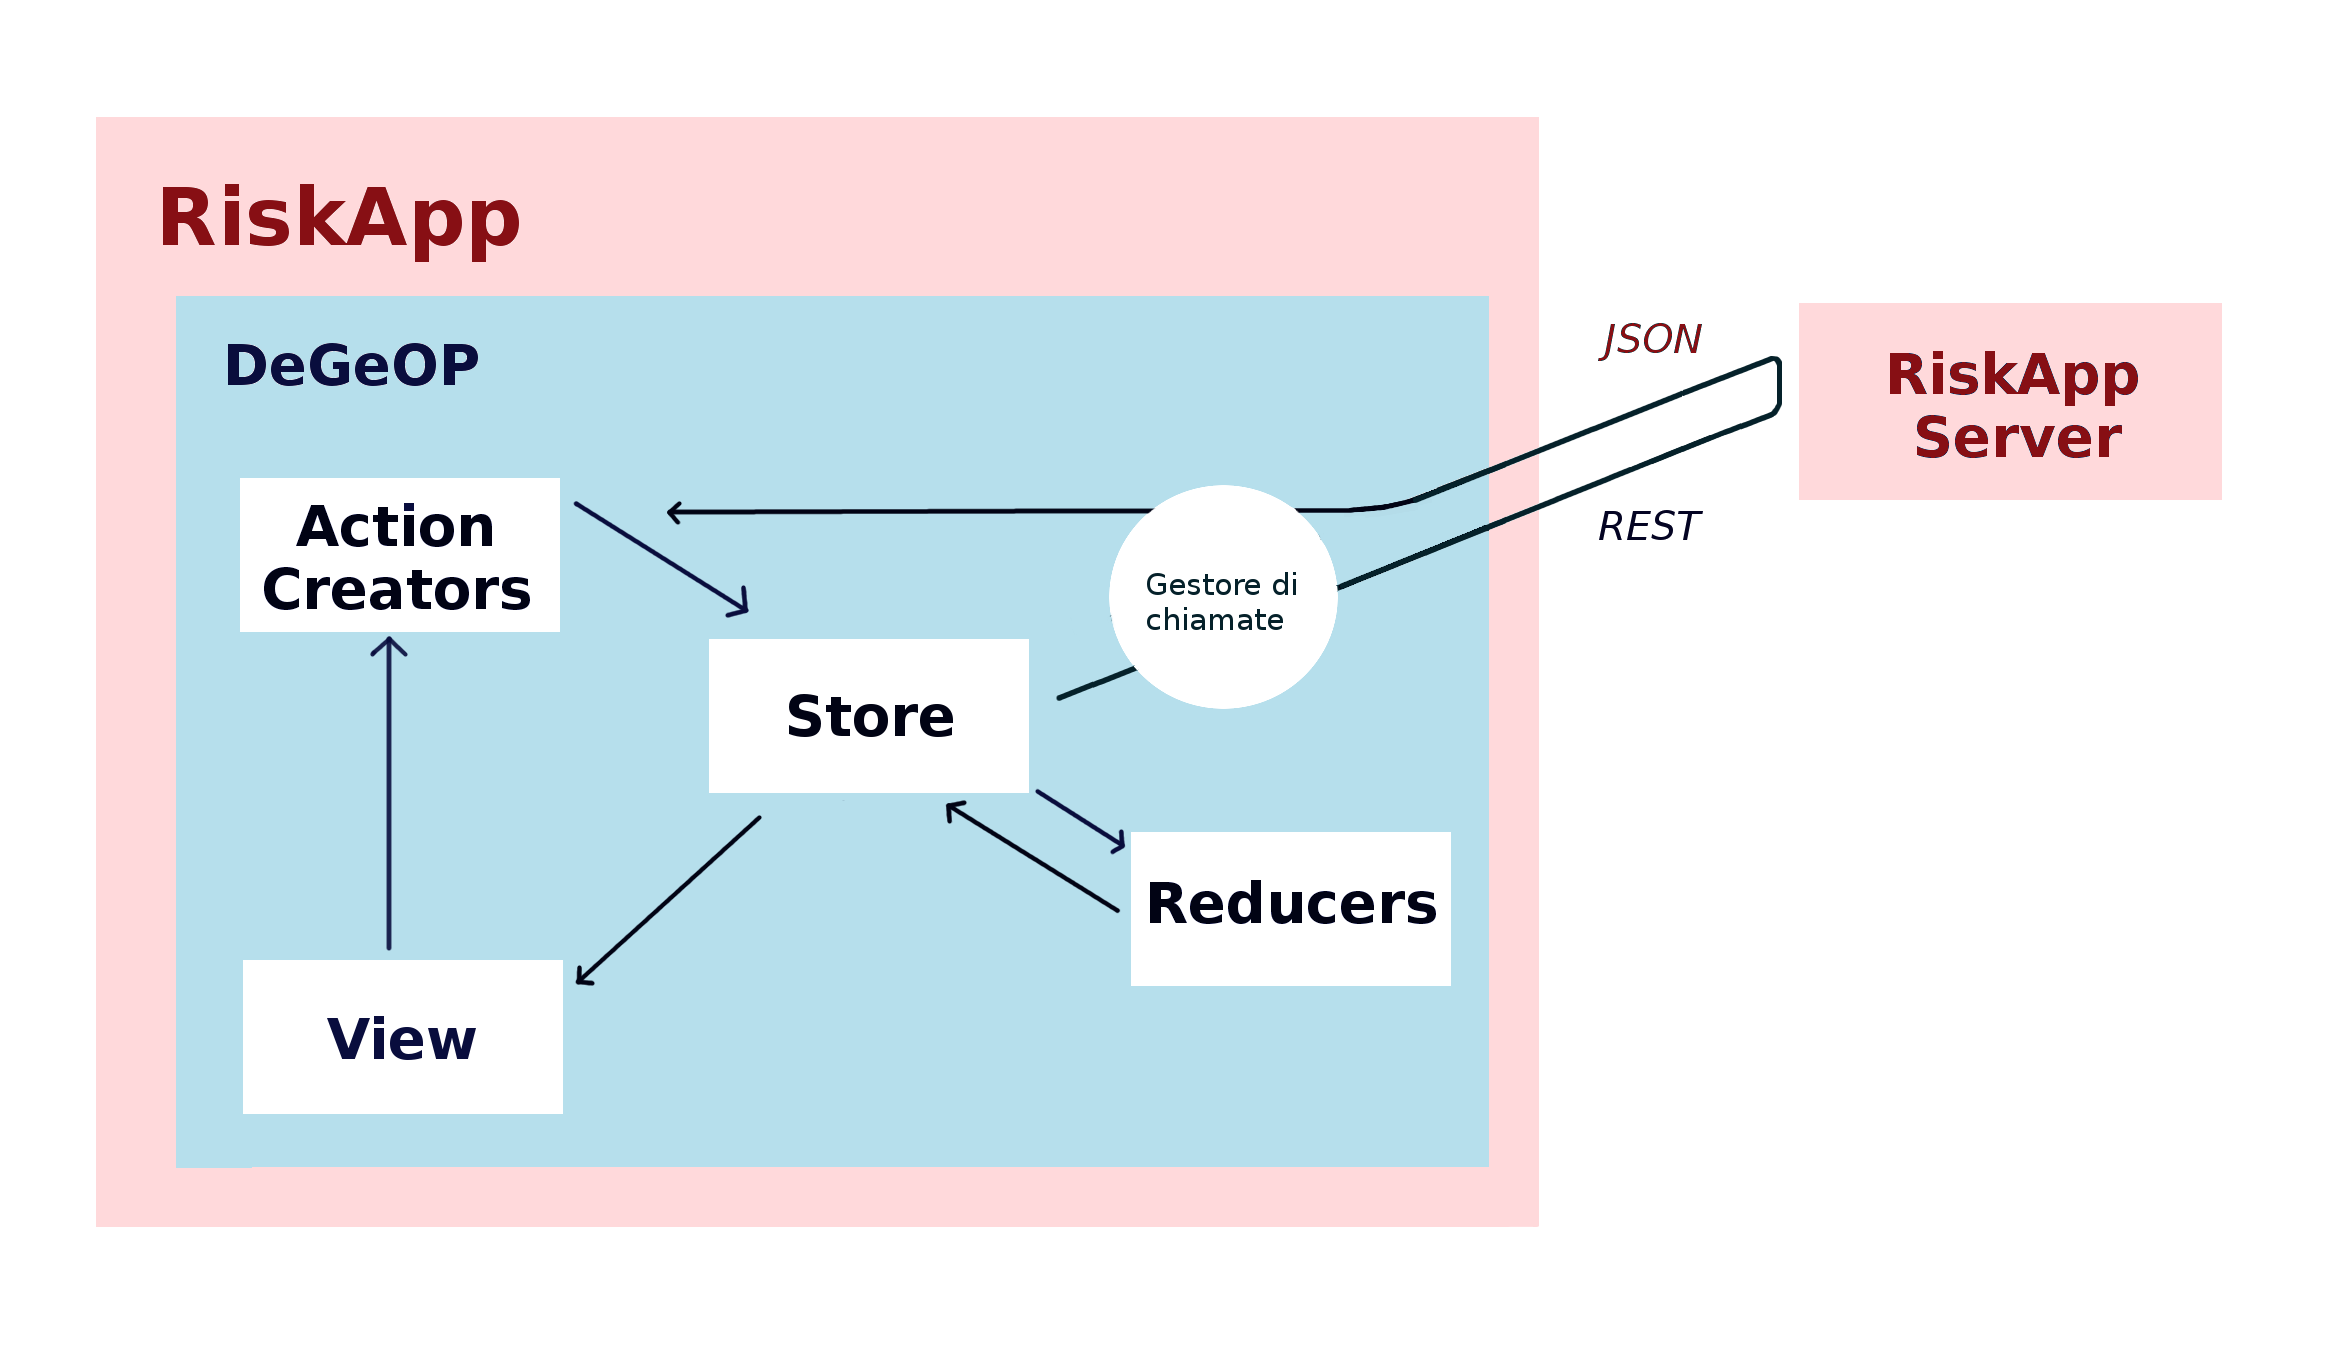
\includegraphics[width=\textwidth]{img/ArchitetturaBase.png}
		\caption{Architettura di base}
	\end{figure}
	%
\section{Componenti}
\subsection{Introduzione}
 Partendo da quanto descritto nel documento di \textit{Specifica Tecnica}, è stato fatto uno studio approfondito delle tecnologie da utilizzare, in modo da poter scendere ad un livello di dettaglio tale da permettere di definire con chiarezza e precisione (seppure mantenendo la sintassi UML) la codifica dell'applicazione da parte dei programmatori.\\
 Questo si nota ed esempio all'interno del \textit{ViewPkg}: l'utilizzo di React, ha permesso:
 \begin{itemize}
	\item buon riutilizzo di codice, consentendo di ridurre fortemente il numero di componenti presentazionali che erano state progettate ad alto livello;
	\item semplificazione della procedura di costruzione dell'interfaccia grafica, grazie al principio di React "lifting state up", che consente la strutturazione dell'interfaccia in maniera fortemente modulare dal punto di vista puramente presentazionale, ma centralizzata dal punto di vista delle informazioni.
\end{itemize}
% v: 17
\subsection{DeGeOP}
\label{pkg::DeGeOP}
\begin{figure}[H]
	\centering
	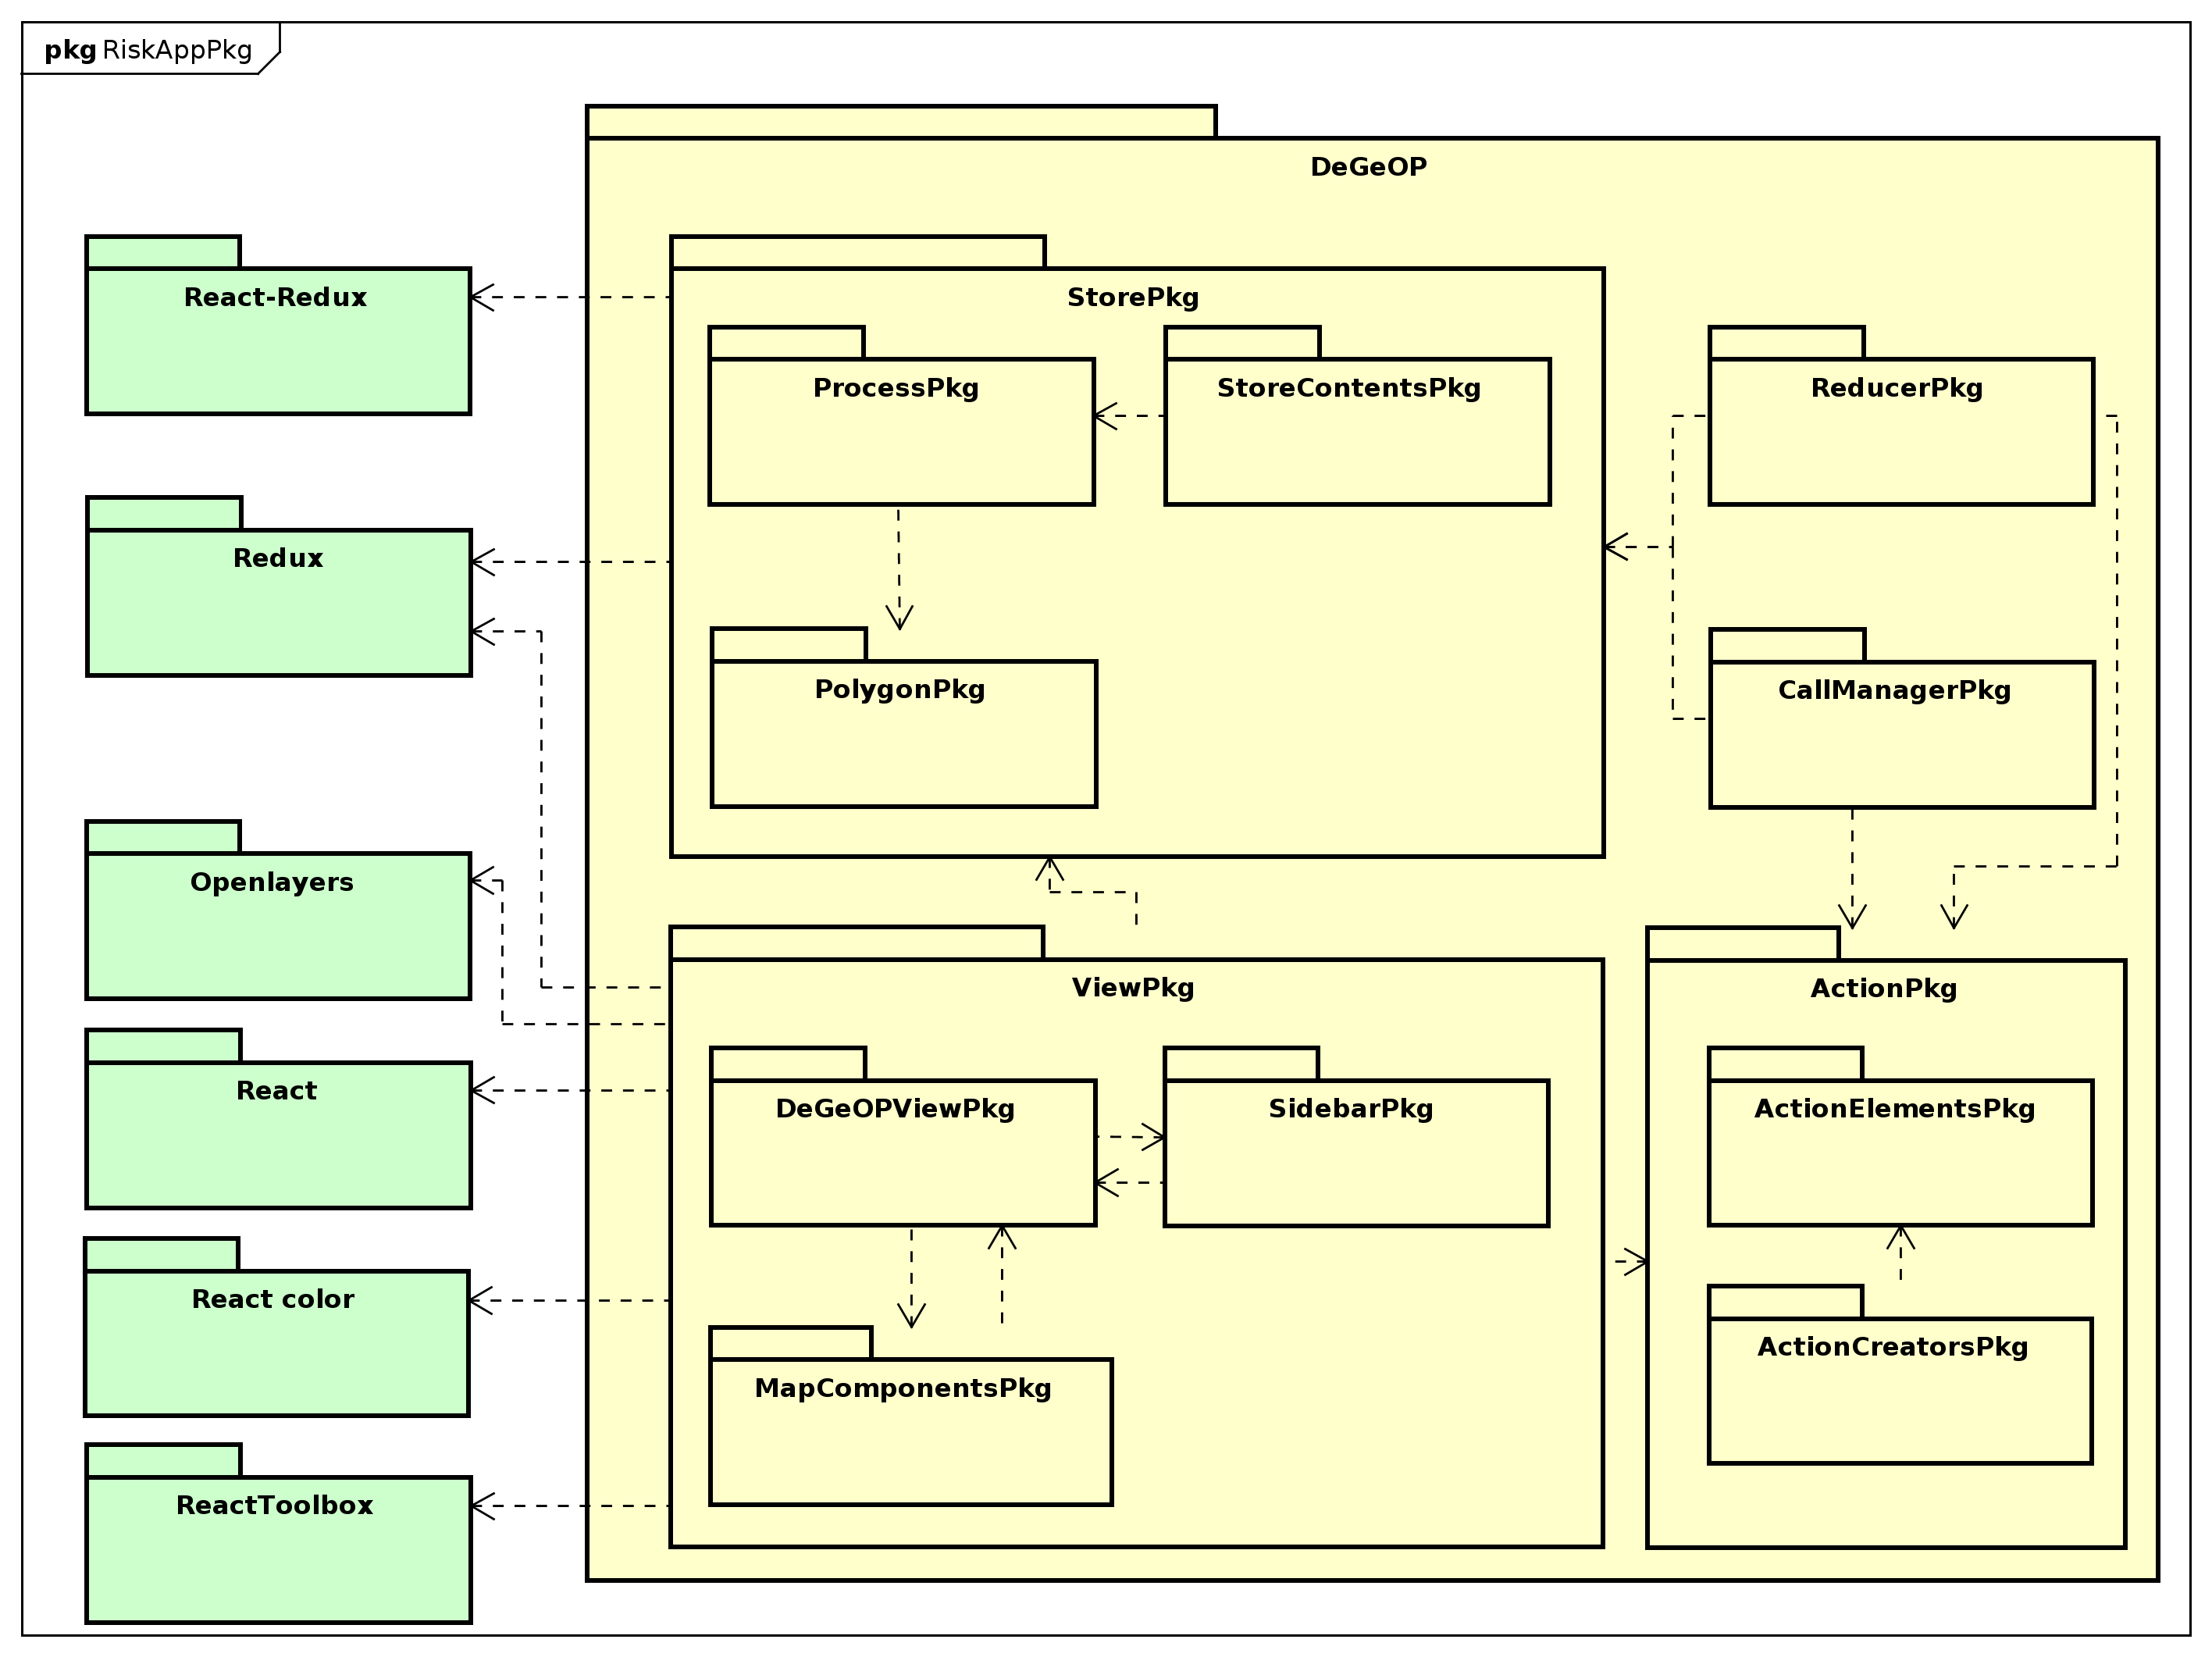
\includegraphics[width=\textwidth]{img/PkgDiagram/DeGeOPPkg.png}
	\caption{Schema componente DeGeOP}
\end{figure}
\subsubsection{Informazioni sul package}
\begin{itemize}
	\item \textbf{descrizione:} racchiude tutte le componenti necessarie per il front-end del prodotto;
	\item \textbf{package contenuti:}
	\begin{itemize}
		\item DeGeOP::\hyperref[pkg::ActionPkg]{ActionPkg};
		\item DeGeOP::\hyperref[pkg::CallManagerPkg]{CallManagerPkg};
		\item DeGeOP::\hyperref[pkg::ReducerPkg]{ReducerPkg};
		\item DeGeOP::\hyperref[pkg::StorePkg]{StorePkg};
		\item DeGeOP::\hyperref[pkg::ViewPkg]{ViewPkg}.
	\end{itemize}
\end{itemize}
\newpage
\subsection{DeGeOP::StorePkg}
\label{pkg::StorePkg}
\begin{figure}[H]
	\centering
	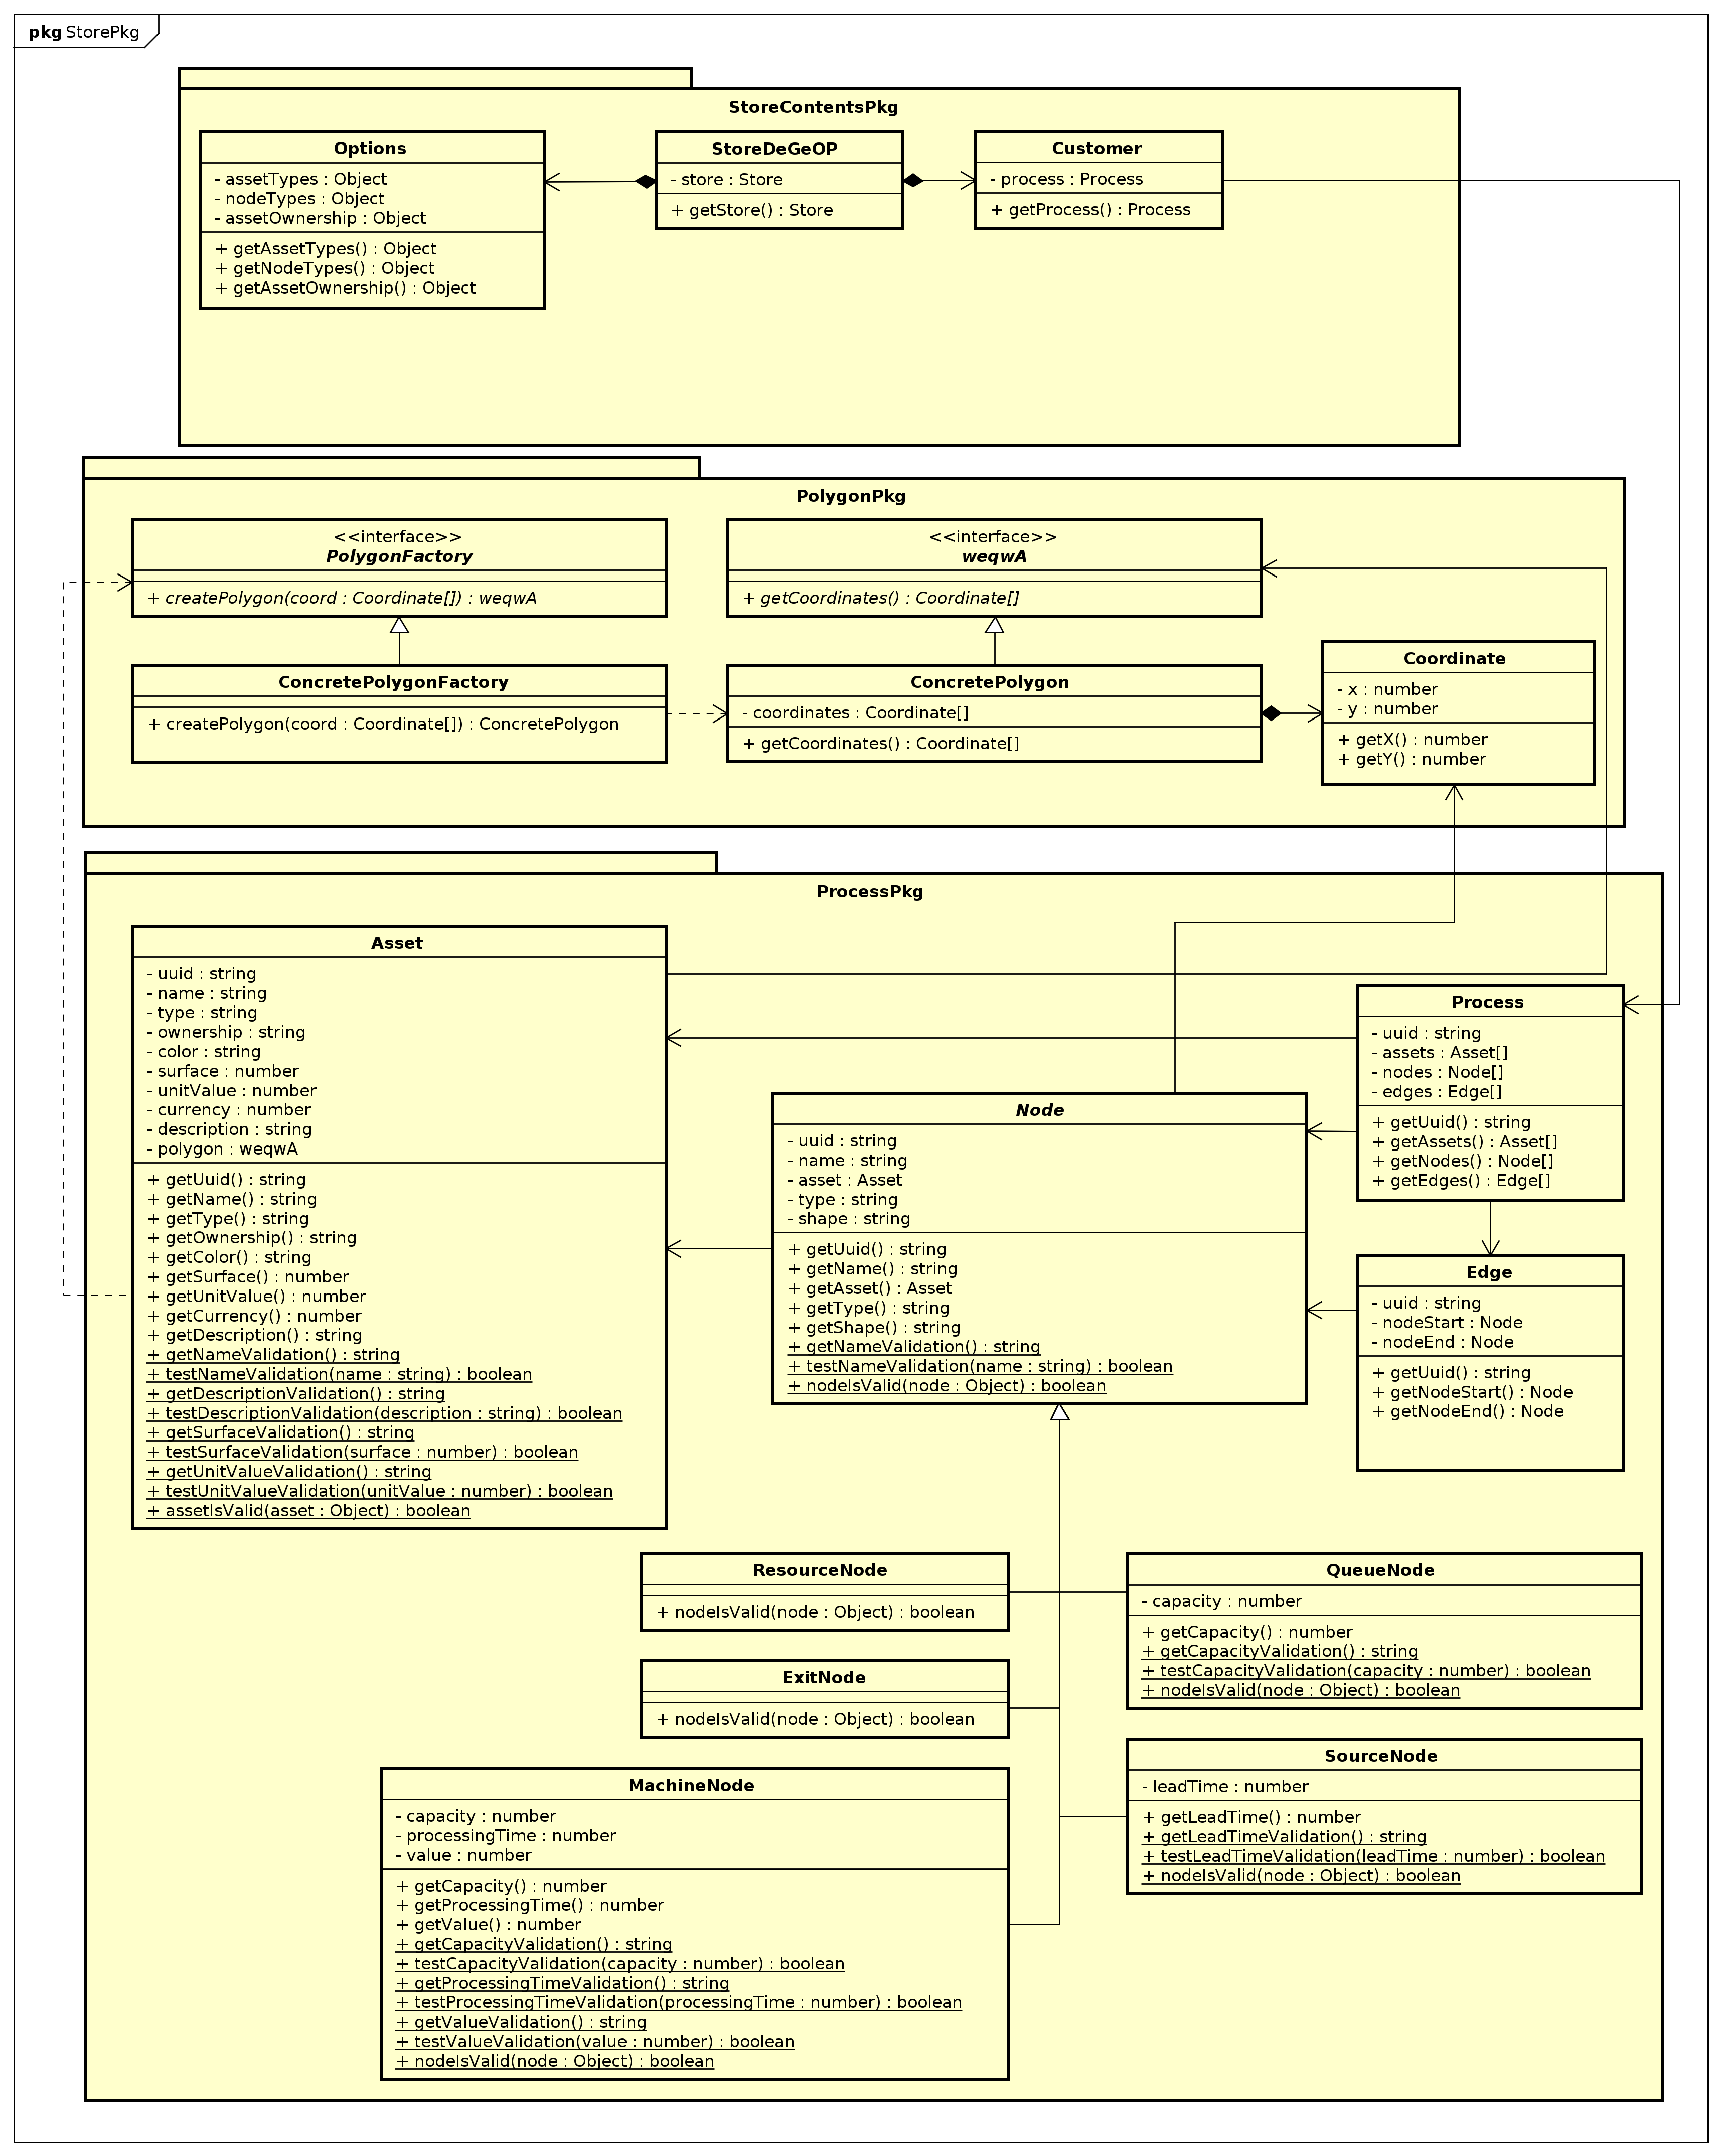
\includegraphics[width=\textwidth]{img/PkgDiagram/StorePkg.png}
	\caption{Schema componente DeGeOP::StorePkg}
\end{figure}
\subsubsection{Informazioni sul package}
\begin{itemize}
	\item \textbf{descrizione:} racchiude le componenti utilizzate per la memorizzazione e rappresentazione dei dati;
	\item \textbf{padre:} \hyperref[pkg::DeGeOP]{DeGeOP};
	\item \textbf{package contenuti:}
	\begin{itemize}
		\item StorePkg::\hyperref[pkg::PolygonPkg]{PolygonPkg};
		\item StorePkg::\hyperref[pkg::ProcessPkg]{ProcessPkg};
		\item StorePkg::\hyperref[pkg::StoreContentsPkg]{StoreContentsPkg}.
	\end{itemize}
	\item \textbf{interazioni con altri package:} 
	\begin{itemize}
		\item IN CallManagerPkg: subscribe sullo store;
		\item IN ReducerPkg: applicazione di cambiamenti di stato;
		\item IN ViewPkg: subscribe sullo store;
		\item OUT React-Redux: utilizzo di Provider per evitare di passare lo store come proprietà alle componenti React;
		\item OUT Redux: creazione Store utilizzando il metodo createStore().
	\end{itemize}
\end{itemize}
\newpage
\subsection{DeGeOP::StorePkg::StoreContentsPkg}
\label{pkg::StoreContentsPkg}
\subsubsection{Informazioni sul package}
\begin{itemize}
	\item \textbf{descrizione:} racchiude le componenti che implementano il concetto di store dell'architettura Redux;
	\item \textbf{padre:} \hyperref[pkg::StorePkg]{StorePkg};
	\item \textbf{interazioni con altri package:} 
	\begin{itemize}
		\item OUT AnalysisPkg: riferimento ad analisi di danno;
		\item OUT ProcessPkg: riferimento a processo;
		\item OUT React-Redux: utilizzo del Provider;
		\item OUT Redux: creazione store.
	\end{itemize}
	\item \textbf{classi contenute:}
	\begin{itemize}
		\item Customer;
		\item Options;
		\item StoreDeGeOP.
	\end{itemize}
\end{itemize}
\subsubsection{Classi}
\paragraph{Customer}
\begin{itemize}
	\begin{figure}[H]
		\centering
		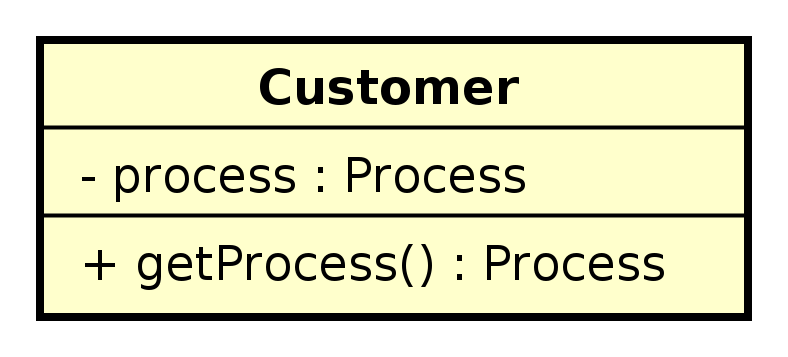
\includegraphics[width=0.3\textwidth]{./img/Customer.png}
		\caption{Diagramma classe Customer}
	\end{figure}
	\item \textbf{descrizione:} rappresenta l'assicurando;
	\item \textbf{utilizzo:} viene utilizzato nello Store per memorizzare l'assicurando;
	\item \textbf{attributi:}
	\begin{itemize}
		\item -process : Process\begin{itemize}
			\item rappresenta il processo produttivo dell'assicurando.\end{itemize}
	\end{itemize}
	\item \textbf{metodi:}
	\begin{itemize}
		\item +getProcess() : Process\newline
		il metodo restituisce il processo produttivo dell'assicurando
	\end{itemize}
\end{itemize}
\paragraph{Options}
\begin{itemize}
	\begin{figure}[H]
		\centering
		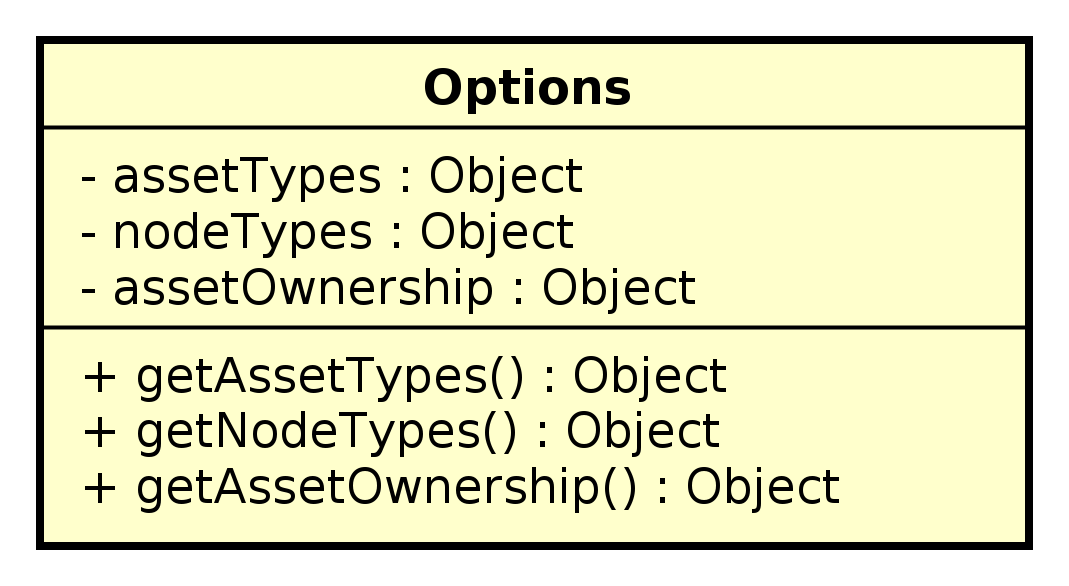
\includegraphics[width=0.3\textwidth]{./img/Options.png}
		\caption{Diagramma classe Options}
	\end{figure}
	\item \textbf{descrizione:} classe contenente le associazioni tra codice e valore dei campi dati degli altri elementi dello store;
	\item \textbf{utilizzo:} viene utilizzata per associare codice e valore dei campi dati degli altri elementi dello store;
	\item \textbf{attributi:}
	\begin{itemize}
		\item -assetOwnership : Object\begin{itemize}
			\item associazione chiave valore delle tipologie di soggetti di appartenenza dell'asset.\end{itemize}
		\item -assetTypes : Object\begin{itemize}
			\item associazione chiave valore delle tipologie di materiale dell'asset.\end{itemize}
		\item -nodeTypes : Object\begin{itemize}
			\item associazione chiave valore delle tipologie di materiale del nodo.\end{itemize}
	\end{itemize}
	\item \textbf{metodi:}
	\begin{itemize}
		\item +getAssetOwnership() : Object\newline
		il metodo ritorna l'oggetto assetOwnership
		\item +getAssetTypes() : Object\newline
		il metodo ritorna l'oggetto assetTypes
		\item +getNodeTypes() : Object\newline
		il metodo ritorna l'oggetto nodeTypes
	\end{itemize}
	\item \textbf{relazioni con altre classi:} 
	\begin{itemize}
		\item IN OptionReducer;
		\item IN StoreDeGeOP.
	\end{itemize}
\end{itemize}
\paragraph{StoreDeGeOP}
\begin{itemize}
	\begin{figure}[H]
		\centering
		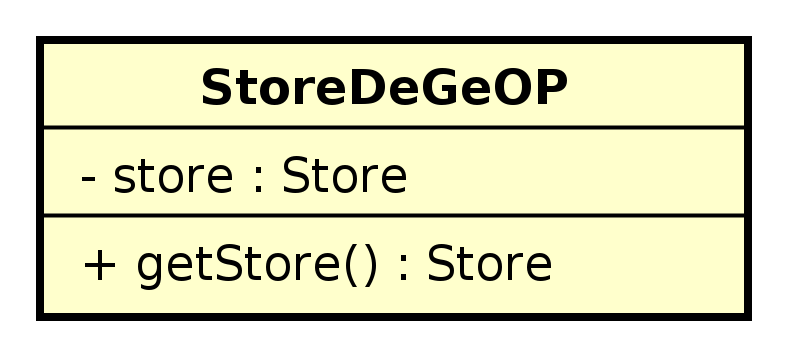
\includegraphics[width=0.3\textwidth]{./img/StoreDeGeOP.png}
		\caption{Diagramma classe StoreDeGeOP}
	\end{figure}
	\item \textbf{descrizione:} rappresenta una classe che incapsula uno Store creato utilizzando Redux;
	\item \textbf{utilizzo:} viene utilizzato per memorizzare lo stato dell'applicazione.
	Le componenti che effettuano il subscribe sullo Store verranno notificate ad ogni cambiamento di stato dello Store;
	\item \textbf{attributi:}
	\begin{itemize}
		\item -customer : Customer\begin{itemize}
			\item rappresenta il cliente che gestiamo.\end{itemize}
		\item -store : Object\begin{itemize}
			\item rappresenta l'oggetto Store creato utilizzando Redux.\end{itemize}
	\end{itemize}
	\item \textbf{metodi:}
	\begin{itemize}
		\item +getStore() : Object\newline
		il metodo restituisce lo store creato utilizzando Redux
	\end{itemize}
	\item \textbf{relazioni con altre classi:} 
	\begin{itemize}
		\item IN Reducer;
		\item OUT Options.
	\end{itemize}
\end{itemize}
\newpage
\subsection{DeGeOP::StorePkg::ProcessPkg}
\label{pkg::ProcessPkg}
\subsubsection{Informazioni sul package}
\begin{itemize}
	\item \textbf{descrizione:} racchiude le componenti necessarie alla rappresentazione del processo produttivo dell'assicurando;
	\item \textbf{padre:} \hyperref[pkg::StorePkg]{StorePkg};
	\item \textbf{interazioni con altri package:} 
	\begin{itemize}
		\item IN StoreContentsPkg: riferimento a processo;
		\item OUT PolygonPkg: riferimento ad un poligono.
	\end{itemize}
	\item \textbf{classi contenute:}
	\begin{itemize}
		\item Asset;
		\item Edge;
		\item ExitNode;
		\item MachineNode;
		\item Node;
		\item Process;
		\item QueueNode;
		\item ResourceNode;
		\item SourceNode.
	\end{itemize}
\end{itemize}
\subsubsection{Classi}
\paragraph{Asset}
\begin{itemize}
	\begin{figure}[H]
		\centering
		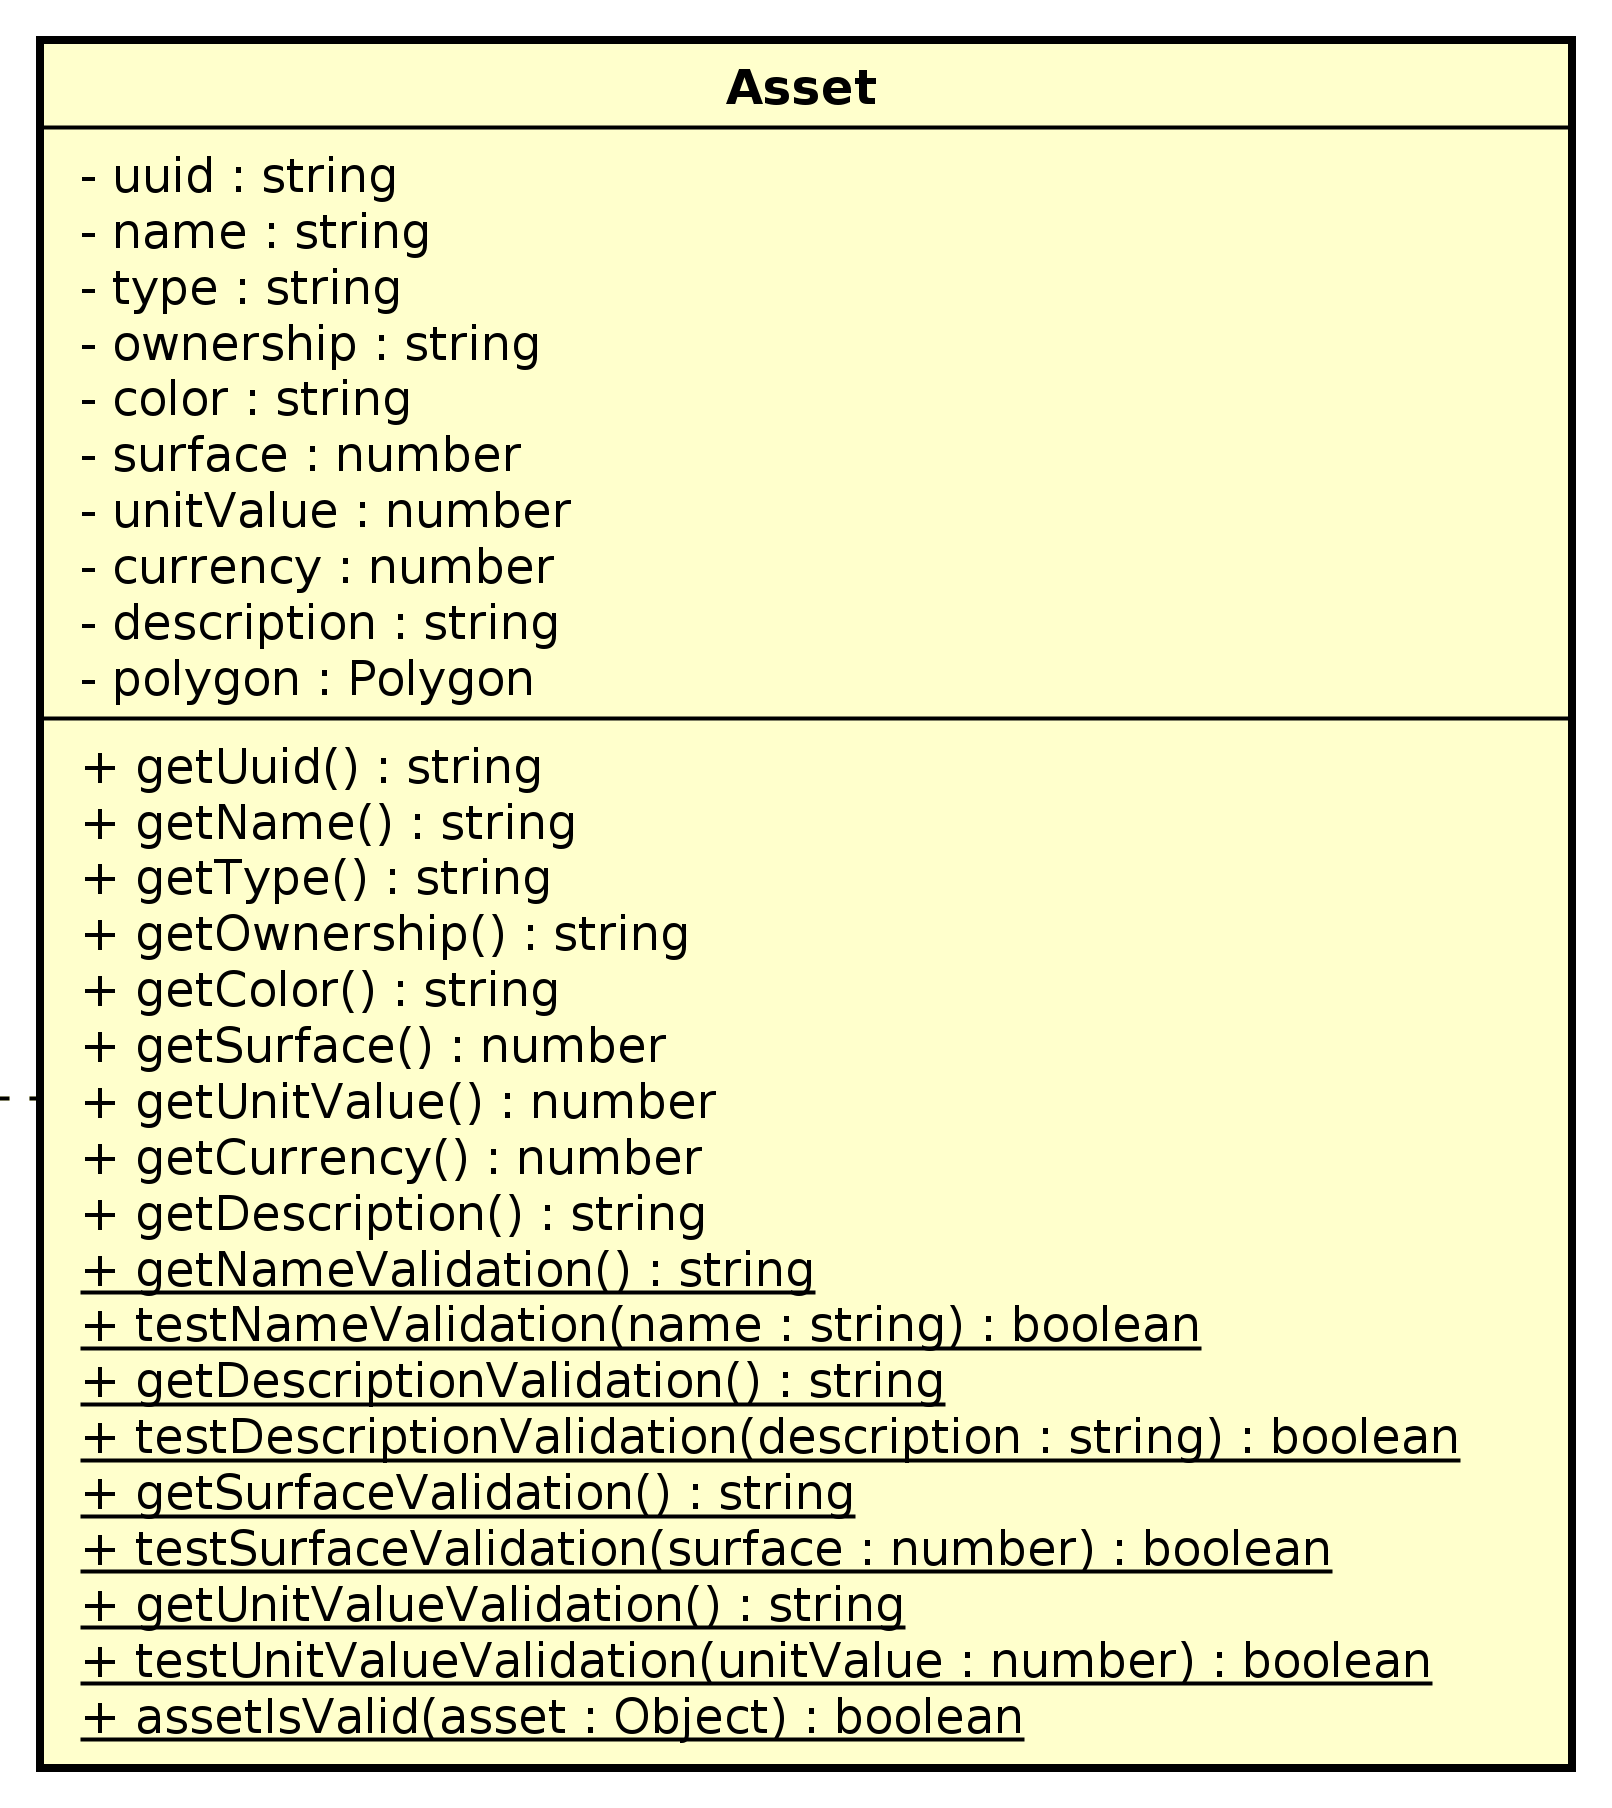
\includegraphics[width=0.3\textwidth]{./img/Asset.png}
		\caption{Diagramma classe Asset}
	\end{figure}
	\item \textbf{descrizione:} rappresenta un fabbricato di interesse per il processo produttivo dell'assicurando;
	\item \textbf{utilizzo:} sono contenuti all'interno di Process;
	\item \textbf{attributi:}
	\begin{itemize}
		\item -color : string\begin{itemize}
			\item indica il colore dell'asset.\end{itemize}
		\item -currency : number\begin{itemize}
			\item indica la valuta utilizzata.\end{itemize}
		\item -description : string\begin{itemize}
			\item rappresenta la descrizione dell'asset.\end{itemize}
		\item -name : string\begin{itemize}
			\item rappresenta il nome dell'asset.\end{itemize}
		\item -ownership : string\begin{itemize}
			\item rappresenta l'appartenenza dell'asset.\end{itemize}
		\item -surface : number\begin{itemize}
			\item rappresenta la dimensione, in mq, dell'asset.\end{itemize}
		\item -type : string\begin{itemize}
			\item rappresenta la tipologia dell'asset.\end{itemize}
		\item -unitValue : string\begin{itemize}
			\item indica il valore economico dell'asset.\end{itemize}
		\item -uuid : string\begin{itemize}
			\item rappresenta l'identificativo dell'asset (uuid).\end{itemize}
	\end{itemize}
	\item \textbf{metodi:}
	\begin{itemize}
		\item +assetIsValid(asset) : boolean\newline
		il metodo testa che i parametri con cui l'asset sta per essere creato siano validi
		\begin{itemize}
			\item asset : Object\\
			oggetto contenente i parametri di un Asset che dovrà essere validato.
		\end{itemize}
		\item +getColor() : string\newline
		il metodo ritorna il colore dell'asset
		\item +getCurrency() : number\newline
		il metodo ritorna la valuta utilizzata per l'asset
		\item +getDescription() : string\newline
		il metodo ritorna la descrizione dell'asset
		\item +getDescriptionValidation() : string\newline
		il metodo ritorna l'espressione regolare che indica una stringa non contenente le seguenti caratteristiche: vuota; più lunga di 5000 caratteri; inizia e/o finisce con uno spazio; contiene caratteri speciali
		diversi dall’apostrofo
		\item +getName() : string\newline
		ritorna il nome dell'asset
		\item +getNameValidation() : string\newline
		il metodo ritorna l'espressione regolare che indica una stringa non contenente le seguenti caratteristiche: più lunga di 50 caratteri; inizia e/o finisce con uno spazio; contiene caratteri speciali.
		\item +getOwnership() : string\newline
		il metodo ritorna l'appartenenza dell'asset
		\item +getSurface() : number\newline
		il metodo ritorna la dimensione dell'asset
		\item +getSurfaceValidation() : string\newline
		il metodo ritorna l'espressione regolare che indica una stringa non contenente le seguenti caratteristiche:vuota; più lunga di 5 cifre per la parte intera; più di 2 per la parte decimale;
		
		\item +getType() : string\newline
		il metodo ritorna la tipologia dell'asset
		\item +getUnitValue() : string\newline
		il metodo ritorna il valore economico dell'asset
		\item +getUnitValueValidation() : string\newline
		il metodo ritorna l'espressione regolare che indica una stringa non contenente le seguenti caratteristiche: vuota; più lunga di 5 cifre per la parte intera; più di 2 per la parte decimale
		\item +getUuid() : string\newline
		il metodo ritorna l'uuid dell'asset
		\item +testDescriptionValidation(description) : boolean\newline
		il metodo ritorna true solamente se il valore ricevuto in input, come parametro, è ritenuto valido.
		\begin{itemize}
			\item description : string\\
			rappresenta la descrizione dell'asset.
		\end{itemize}
		\item +testNameValidation(name) : boolean\newline
		il metodo ritorna true solamente se il valore ricevuto in input, come parametro, è ritenuto valido.
		\begin{itemize}
			\item name : string\\
			rappresenta il nome dell'asset.
		\end{itemize}
		\item +testSurfaceValidation(surface) : boolean\newline
		il metodo ritorna true solamente se il valore ricevuto in input, come parametro, è ritenuto valido.
		\begin{itemize}
			\item surface : number\\
			rappresenta la dimensione, in mq, dell'asset.
		\end{itemize}
		\item +testUnitValueValidation(unitValue) : boolean\newline
		il metodo ritorna true solamente se il valore ricevuto in input, come parametro, è ritenuto valido.
		\begin{itemize}
			\item unitValue : number\\
			indica il valore economico dell'asset.
		\end{itemize}
	\end{itemize}
	\item \textbf{relazioni con altre classi:} 
	\begin{itemize}
		\item IN AssetReducer.
	\end{itemize}
\end{itemize}
\paragraph{Edge}
\begin{itemize}
	\begin{figure}[H]
		\centering
		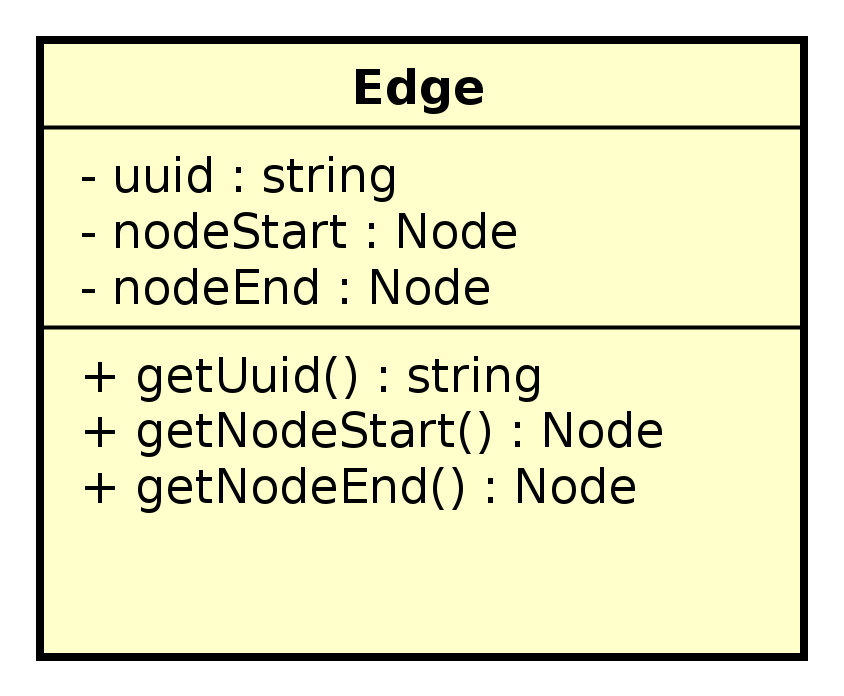
\includegraphics[width=0.3\textwidth]{./img/Edge.png}
		\caption{Diagramma classe Edge}
	\end{figure}
	\item \textbf{descrizione:} rappresenta un arco che collega due nodi tra di loro; un arco indica che i nodi sono in correlazione tra di loro;
	\item \textbf{utilizzo:} è contenuto all'interno di Process;
	\item \textbf{attributi:}
	\begin{itemize}
		\item -nodeEnd : Node\begin{itemize}
			\item rappresenta il nodo di arrivo.\end{itemize}
		\item -nodeStart : Node\begin{itemize}
			\item rappresenta il nodo di partenza.\end{itemize}
		\item -uuid : string\begin{itemize}
			\item rappresenta il codice identificativo dell'arco (uuid).\end{itemize}
	\end{itemize}
	\item \textbf{metodi:}
	\begin{itemize}
		\item +getNodeEnd() : Node\newline
		il metodo restituisce il nodo di arrivo
		\item +getNodeStart() : Node\newline
		il metodo restituisce il nodo di partenza
		\item +getUuid() : string\newline
		il metodo restituisce il codice identificativo dell'arco (uuid)
	\end{itemize}
	\item \textbf{relazioni con altre classi:} 
	\begin{itemize}
		\item IN EdgeReducer.
	\end{itemize}
\end{itemize}
\paragraph{ExitNode}
\begin{itemize}
	\begin{figure}[H]
		\centering
		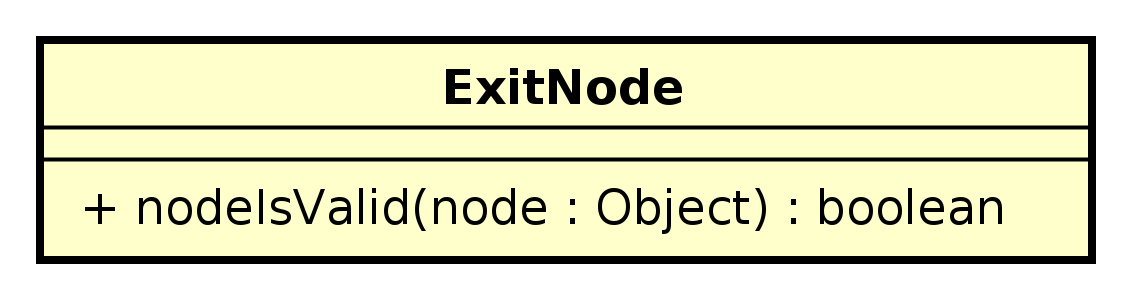
\includegraphics[width=0.3\textwidth]{./img/ExitNode.png}
		\caption{Diagramma classe ExitNode}
	\end{figure}
	\item \textbf{descrizione:} rappresenta un nodo di tipo Uscita;
	\item \textbf{utilizzo:} è contenuto all'interno di Process;
	\item \textbf{metodi:}
	\begin{itemize}
		\item +nodeIsValid() : boolean\newline
		il metodo testa che i parametri con cui il nodo sta per essere creato siano validi
	\end{itemize}
\end{itemize}
\paragraph{MachineNode}
\begin{itemize}
	\begin{figure}[H]
		\centering
		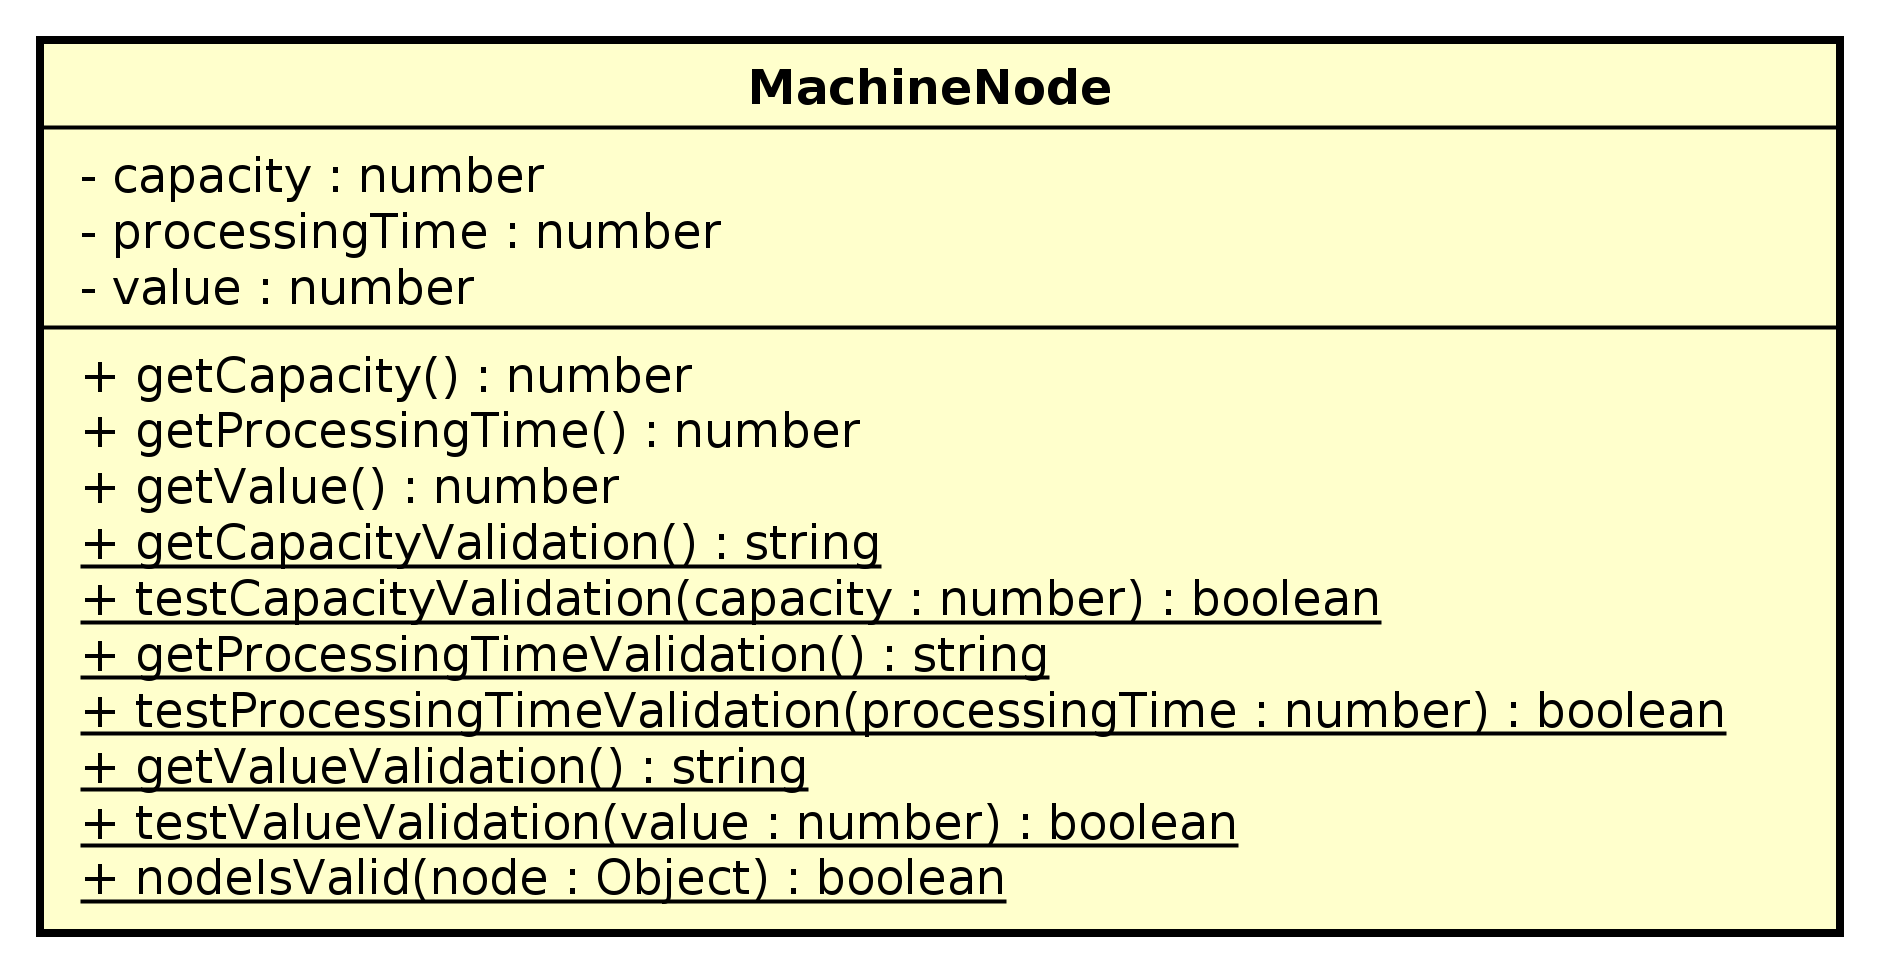
\includegraphics[width=0.3\textwidth]{./img/MachineNode.png}
		\caption{Diagramma classe MachineNode}
	\end{figure}
	\item \textbf{descrizione:} rappresenta un nodo di tipo Macchina;
	\item \textbf{utilizzo:} è contenuto all'interno di Process;
	\item \textbf{attributi:}
	\begin{itemize}
		\item -capacity : number\begin{itemize}
			\item rappresenta la capacità del nodo.\end{itemize}
		\item -processingTime : number\begin{itemize}
			\item rappresenta il tempo di processo del nodo.\end{itemize}
		\item -value : number\begin{itemize}
			\item rappresenta il valore del nodo.\end{itemize}
	\end{itemize}
	\item \textbf{metodi:}
	\begin{itemize}
		\item +getCapacity() : number\newline
		il metodo ritorna la capacità del nodo
		\item +getCapacityValidation() : string\newline
		il metodo ritorna l'espressione regolare che indica una stringa non contenente le seguenti caratteristiche: vuota; più lunga di 5 cifre per la parte intera; più di 2 per la parte decimale;
		\item +getProcessingTime() : number\newline
		il metodo ritorna il tempo di processo del nodo
		\item +getProcessingTimeValidation() : string\newline
		il metodo ritorna l'espressione regolare che indica una stringa non contenente le seguenti caratteristiche: vuota; più lunga di 5 cifre per la parte intera; più di 2 per la parte decimale;
		\item +getValue() : number\newline
		il metodo ritorna il valore del nodo
		\item +getValueValidation() : string\newline
		il metodo ritorna l'espressione regolare che indica una stringa non contenente le seguenti caratteristiche: vuota; più lunga di 20 cifre per la parte intera; più di 2 per la parte decimale
		\item +nodeIsValid(node) : boolean\newline
		il metodo testa se i parametri con cui il nodo sta per essere creato sono validi
		\begin{itemize}
			\item node : Object\\
			oggetto che rappresenta i parametri con cui il nodo sta per essere creato.
		\end{itemize}
		\item +testCapacityValidation() : boolean\newline
		il metodo testa se la capacità del nodo valida
		\item +testProcessingTimeValidation(processingTime) : boolean\newline
		il metodo testa se il tempo di processo valida
		\begin{itemize}
			\item processingTime : number\\
			rappresenta il tempo di processo del nodo.
		\end{itemize}
		\item +testValueValidation(value) : boolean\newline
		il metodo testa se il valore del nodo valida
		\begin{itemize}
			\item value : number\\
			rappresenta il valore del nodo.
		\end{itemize}
	\end{itemize}
\end{itemize}
\paragraph{Node}
\begin{itemize}
	\begin{figure}[H]
		\centering
		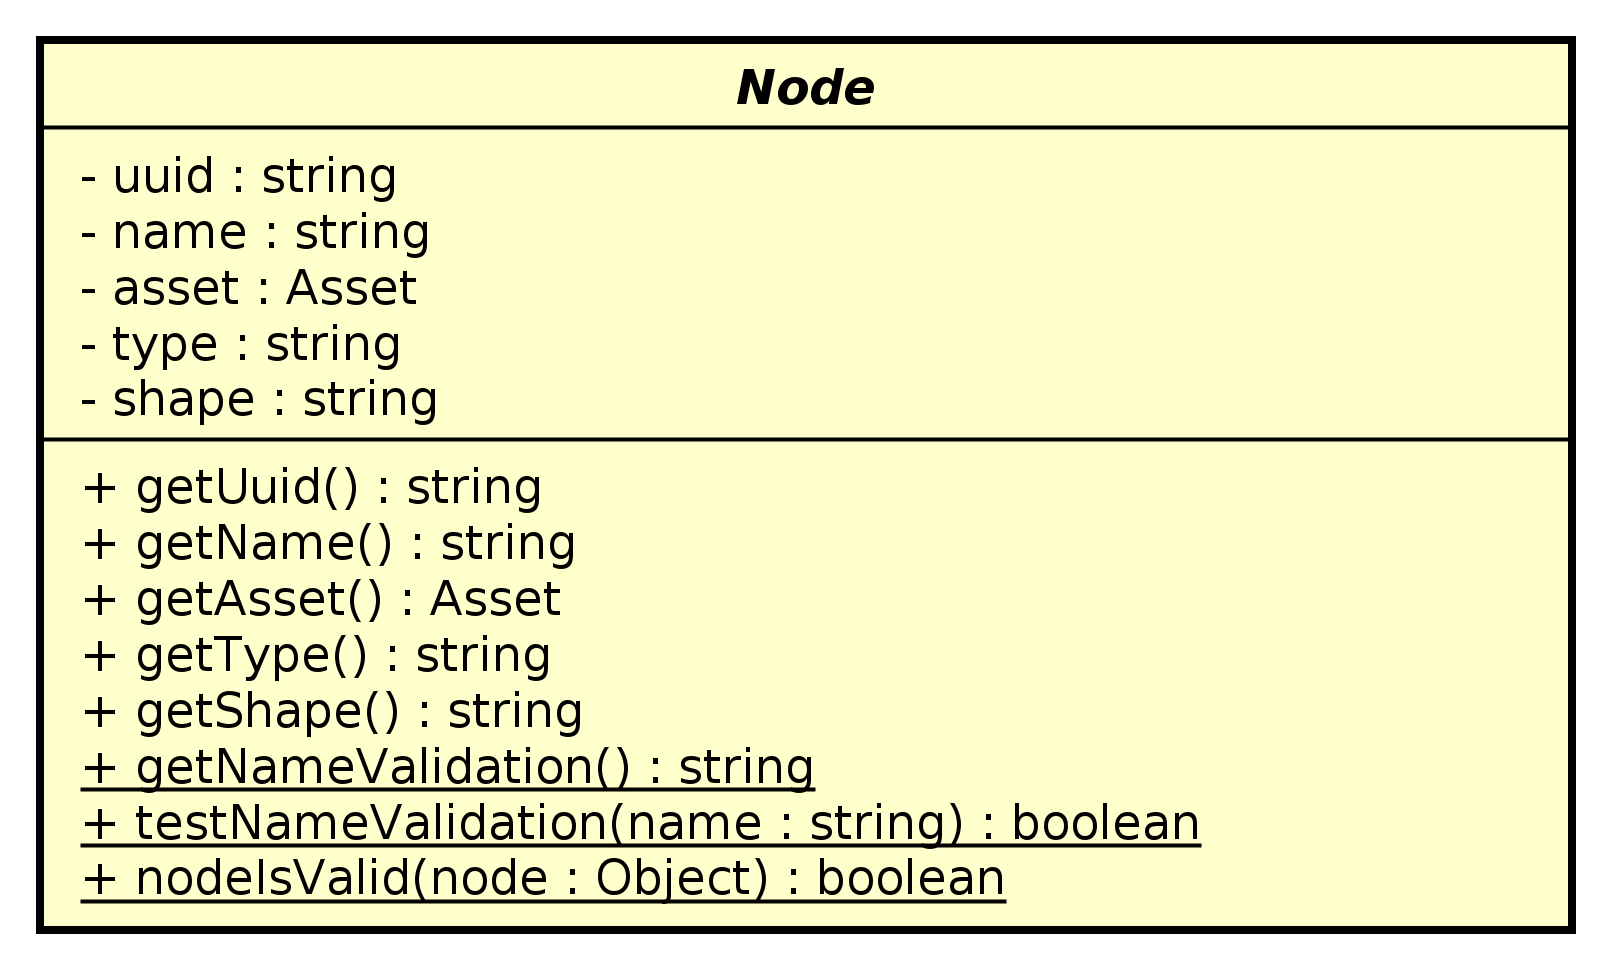
\includegraphics[width=0.3\textwidth]{./img/Node.png}
		\caption{Diagramma classe Node}
	\end{figure}
	\item \textbf{descrizione:} rappresenta un nodo contenuto all'interno di un Asset ;
	\item \textbf{utilizzo:} è contenuto all'interno di Process;
	\item \textbf{attributi:}
	\begin{itemize}
		\item -asset : Asset\begin{itemize}
			\item rappresenta l'asset a cui il nodo appartiene.\end{itemize}
		\item -name : string\begin{itemize}
			\item rappresenta il nome del nodo.\end{itemize}
		\item -shape : string\begin{itemize}
			\item rappresenta la forma del nodo.\end{itemize}
		\item -type : string\begin{itemize}
			\item rappresenta la classe del nodo.\end{itemize}
		\item -uuid : string\begin{itemize}
			\item rappresenta il codice identificativo del nodo (uuid).\end{itemize}
	\end{itemize}
	\item \textbf{metodi:}
	\begin{itemize}
		\item +getAsset() : Asset\newline
		il metodo ritorna l'asset di appartenenza del nodo
		\item +getName() : string\newline
		il metodo ritorna il codice identificativo del nodo
		\item +getNameValidation() : string\newline
		il metodo ritorna l'espressione regolare che indica una stringa non contenente le seguenti caratteristiche: vuota; più
		lunga di 50 caratteri; inizia e/o finisce con uno spazio; contiene caratteri speciali;
		\item +getShape() : string\newline
		il metodo ritorna la forma del nodo
		\item +getType() : string\newline
		il metodo ritorna la classe del nodo
		\item +getUuid() : string\newline
		il metodo ritorna il codice identificativo del nodo (uuid)
		\item +nodeIsValid() : boolean\newline
		il metodo testa che i parametri con cui il nodo sta per essere creato siano validi
		\item +testNameValidation(name) : boolean\newline
		il metodo ritorna true solamente se il valore ricevuto in input, come parametro, è ritenuto valido.
		\begin{itemize}
			\item name : string\\
			rappresenta il nome del nodo.
		\end{itemize}
	\end{itemize}
	\item \textbf{relazioni con altre classi:} 
	\begin{itemize}
		\item IN NodeReducer.
	\end{itemize}
\end{itemize}
\paragraph{Process}
\begin{itemize}
	\begin{figure}[H]
		\centering
		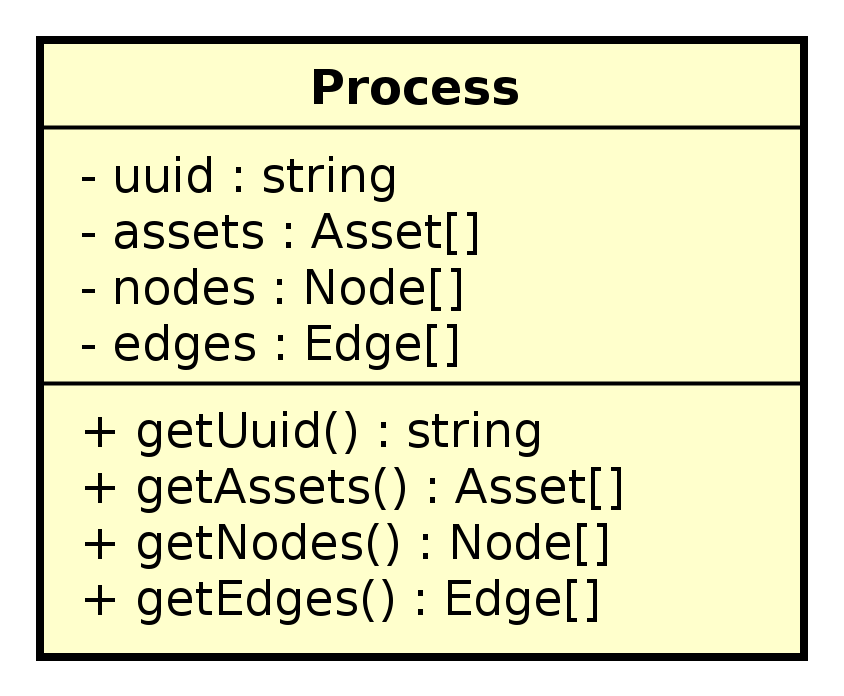
\includegraphics[width=0.3\textwidth]{./img/Process.png}
		\caption{Diagramma classe Process}
	\end{figure}
	\item \textbf{descrizione:} rappresenta un processo produttivo dell'azienda dell'assicurando;
	\item \textbf{utilizzo:} è memorizzato nello Store;
	\item \textbf{attributi:}
	\begin{itemize}
		\item -assets : Asset[ ]\begin{itemize}
			\item rappresenta gli asset facenti parti del processo produttivo.\end{itemize}
		\item -edges : Edge [ ]\begin{itemize}
			\item rappresenta gli archi che effettuano i collegamenti nel processo produttivo.\end{itemize}
		\item -nodes : Node [ ]\begin{itemize}
			\item rappresenta i nodi facenti parti del processo produttivo.\end{itemize}
		\item -uuid : string\begin{itemize}
			\item rappresenta l'identificativo del processo (uuid).\end{itemize}
	\end{itemize}
	\item \textbf{metodi:}
	\begin{itemize}
		\item +getAssets() : Asset[ ]\newline
		il metodo ritorna gli asset facenti parti del processo produttivo
		\item +getEdges() : Edge [ ]\newline
		il metodo ritorna gli archi che effettuano i collegamenti nel processo produttivo
		\item +getNodes() : Node [ ]\newline
		il metodo ritorna i nodi facenti parti del processo produttivo
		\item +getUuid() : string\newline
		il metodo ritorna il codice identificativo (uuid) del processo
	\end{itemize}
\end{itemize}
\paragraph{QueueNode}
\begin{itemize}
	\begin{figure}[H]
		\centering
		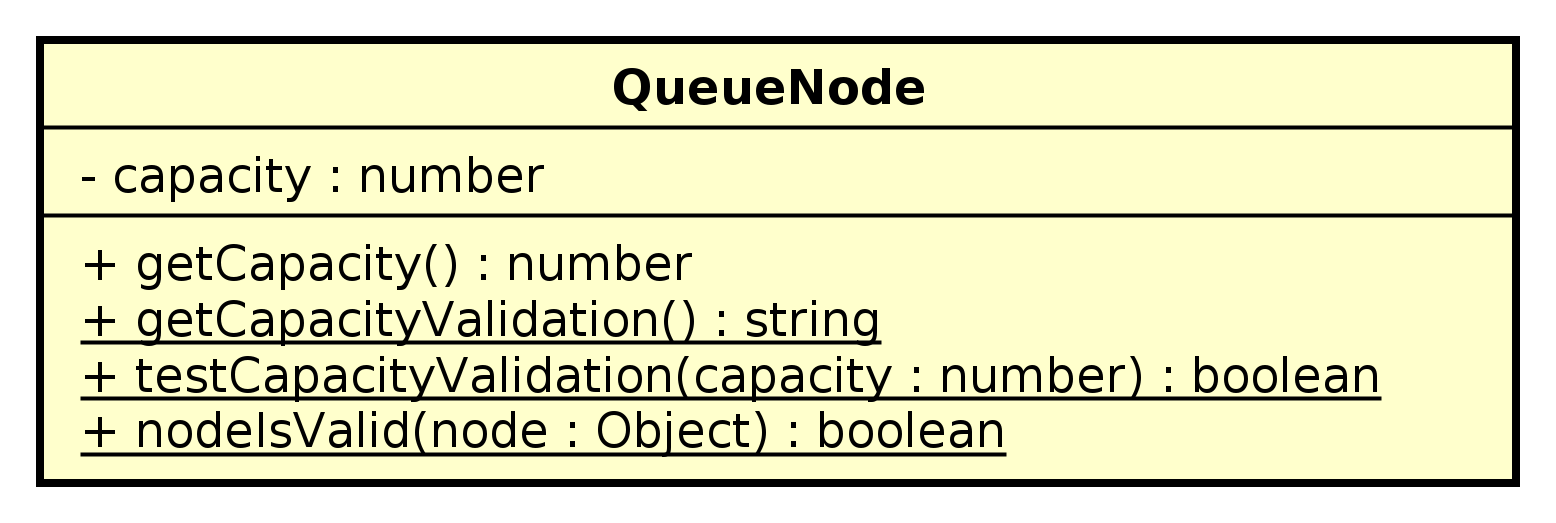
\includegraphics[width=0.3\textwidth]{./img/QueueNode.png}
		\caption{Diagramma classe QueueNode}
	\end{figure}
	\item \textbf{descrizione:} rappresenta un nodo di tipo Coda;
	\item \textbf{utilizzo:} è contenuto all'interno di Process;
	\item \textbf{attributi:}
	\begin{itemize}
		\item -capacity : number\begin{itemize}
			\item rappresenta la capacità del nodo coda.\end{itemize}
	\end{itemize}
	\item \textbf{metodi:}
	\begin{itemize}
		\item +getCapacity() : number\newline
		il metodo ritorna la capacità del nodo
		\item +getCapacityValidation() : string\newline
		il metodo ritorna l'espressione regolare che indica una stringa non contenente le seguenti caratteristiche: vuota; più lunga di 5 cifre per la parte intera; più di 2 per la parte decimale;
		\item +nodeIsValid(node) : boolean\newline
		il metodo testa che i parametri con cui il nodo sta per essere creato siano validi
		\begin{itemize}
			\item node : Object\\
			oggetto che rappresenta i parametri con cui il nodo sta per essere creato.
		\end{itemize}
		\item +testCapacityValidation(capacity) : boolean\newline
		il metodo ritorna true solamente se il valore ricevuto in input, come parametro, è ritenuto valido.
		\begin{itemize}
			\item capacity : number\\
			rappresenta la capacità del nodo.
		\end{itemize}
	\end{itemize}
\end{itemize}
\paragraph{ResourceNode}
\begin{itemize}
	\begin{figure}[H]
		\centering
		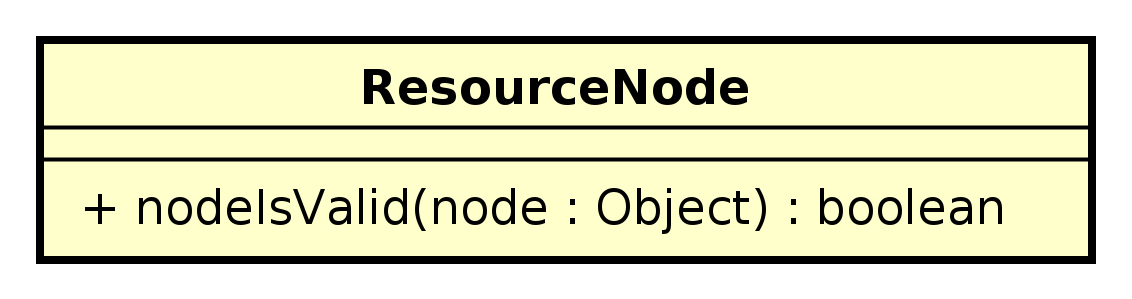
\includegraphics[width=0.3\textwidth]{./img/ResourceNode.png}
		\caption{Diagramma classe ResourceNode}
	\end{figure}
	\item \textbf{descrizione:} rappresenta un nodo di tipo Risorsa;
	\item \textbf{utilizzo:} è contenuto all'interno di Process;
	\item \textbf{metodi:}
	\begin{itemize}
		\item +nodeIsValid() : boolean\newline
		il metodo testa che i parametri con cui il nodo sta per essere creato siano validi
	\end{itemize}
\end{itemize}
\paragraph{SourceNode}
\begin{itemize}
	\begin{figure}[H]
		\centering
		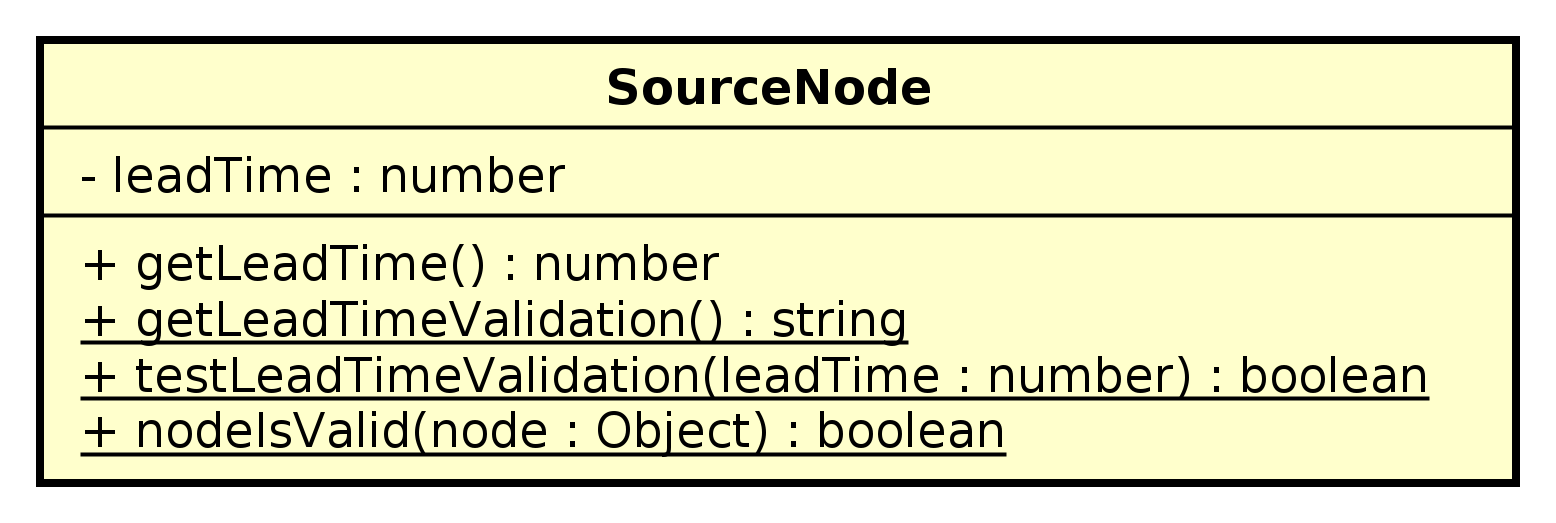
\includegraphics[width=0.3\textwidth]{./img/SourceNode.png}
		\caption{Diagramma classe SourceNode}
	\end{figure}
	\item \textbf{descrizione:} rappresenta un nodo di tipo Sorgente;
	\item \textbf{utilizzo:} è contenuto all'interno di Process;
	\item \textbf{attributi:}
	\begin{itemize}
		\item -leadTime : Object\begin{itemize}
			\item rappresenta il tempo di approvvigionamento del nodo.\end{itemize}
	\end{itemize}
	\item \textbf{metodi:}
	\begin{itemize}
		\item +getLeadTime() : number\newline
		il metodo ritorna il tempo di approvigionamento del nodo
		\item +getLeadTimeValidation() : string\newline
		il metodo ritorna l'espressione regolare che indica una stringa non contenente le seguenti caratteristiche: vuota; più lunga di 5 cifre per la parte intera; più di 2 per la parte decimale;
		\item +nodeIsValid(node) : boolean\newline
		il metodo testa se i parametri con cui il nodo sta per essere creato sono validi
		\begin{itemize}
			\item node : Object\\
			oggetto che rappresenta i parametri con cui il nodo sta per essere creato.
		\end{itemize}
		\item +testLeadTimeValidation(leadTime) : boolean\newline
		il metodo testa se il tempo di approvvigionamento è valido
		\begin{itemize}
			\item leadTime : number\\
			rappresenta il tempo di approvvigionamento.
		\end{itemize}
	\end{itemize}
\end{itemize}
\newpage
\subsection{DeGeOP::StorePkg::PolygonPkg}
\label{pkg::PolygonPkg}
\subsubsection{Informazioni sul package}
\begin{itemize}
	\item \textbf{descrizione:} racchiude le componenti necessarie alla rappresentazione dell'area degli asset e degli scenari di danno;
	\item \textbf{padre:} \hyperref[pkg::StorePkg]{StorePkg};
	\item \textbf{interazioni con altri package:} 
	\begin{itemize}
		\item IN AnalysisPkg: riferimento ad un poligono;
		\item IN ProcessPkg: riferimento ad un poligono.
	\end{itemize}
	\item \textbf{classi contenute:}
	\begin{itemize}
		\item ConcretePolygon;
		\item ConcretePolygonFactory;
		\item Coordinate;
		\item Polygon;
		\item PolygonFactory.
	\end{itemize}
\end{itemize}
\subsubsection{Classi}
\paragraph{ConcretePolygon}
\begin{itemize}
	\begin{figure}[H]
		\centering
		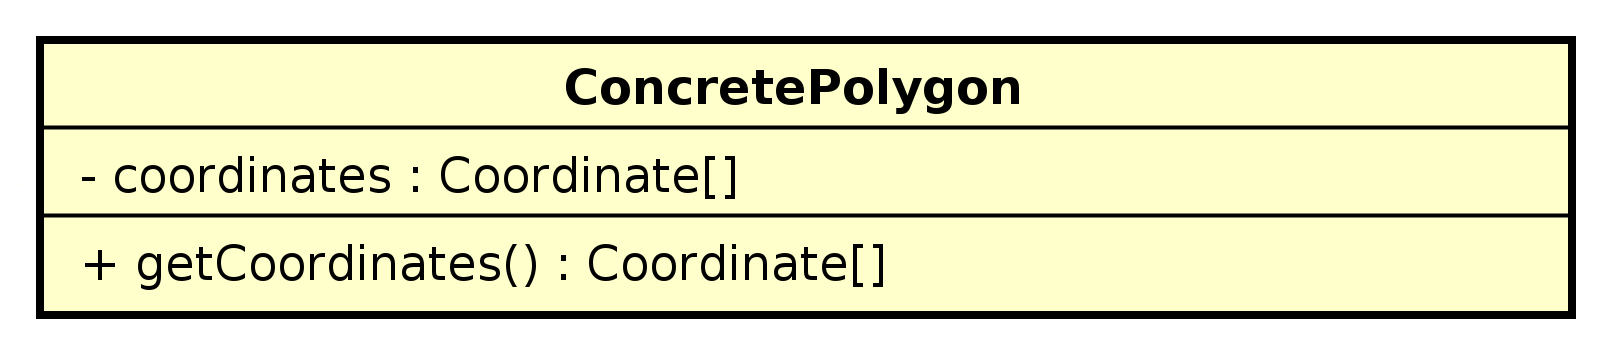
\includegraphics[width=0.3\textwidth]{./img/ConcretePolygon.png}
		\caption{Diagramma classe ConcretePolygon}
	\end{figure}
	\item \textbf{descrizione:} rappresenta un poligono;
	\item \textbf{utilizzo:} viene istanziata da ConcretePolygonFactory; viene utilizzata in Asset e Scenario;
	\item \textbf{attributi:}
	\begin{itemize}
		\item -coordinates : Coordinate[]\begin{itemize}
			\item rappresenta le coordinate che vanno a delineare il poligono.\end{itemize}
	\end{itemize}
	\item \textbf{metodi:}
	\begin{itemize}
		\item +getCoordinates() : Coordinate[]\newline
		il metodo restituisce le coordinate che vanno a delineare il poligono
	\end{itemize}
\end{itemize}
\paragraph{ConcretePolygonFactory}
\begin{itemize}
	\begin{figure}[H]
		\centering
		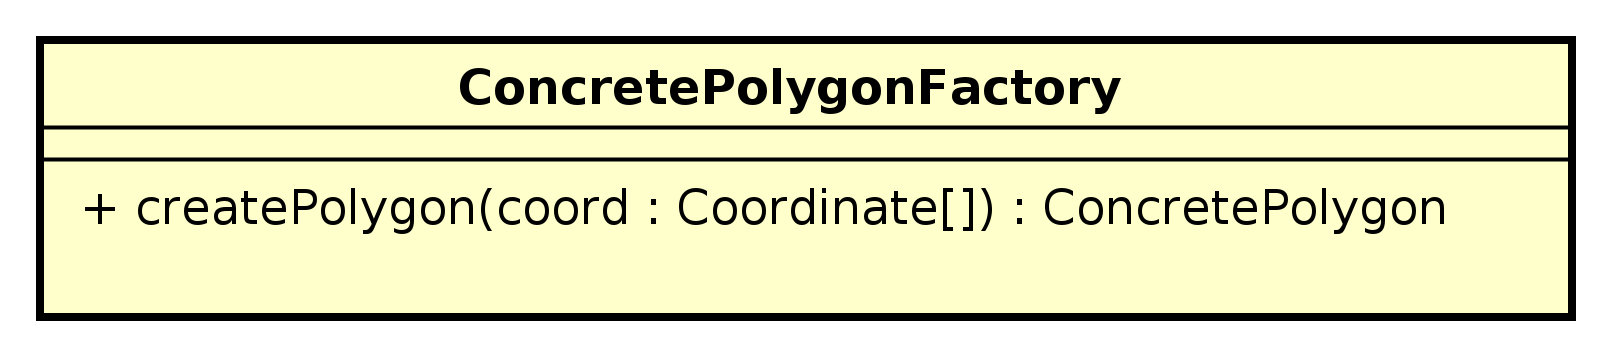
\includegraphics[width=0.3\textwidth]{./img/ConcretePolygonFactory.png}
		\caption{Diagramma classe ConcretePolygonFactory}
	\end{figure}
	\item \textbf{descrizione:} gestisce la creazione concreta dei poligoni;
	\item \textbf{utilizzo:} implementazione di PolygonFactory; è la classe concreta da istanziare per gestire la creazione di un poligono;
	\item \textbf{metodi:}
	\begin{itemize}
		\item +createPolygon() : ConcretePolygon\newline
		il metodo si occupa della costruzione del poligono
	\end{itemize}
\end{itemize}
\paragraph{Coordinate}
\begin{itemize}
	\begin{figure}[H]
		\centering
		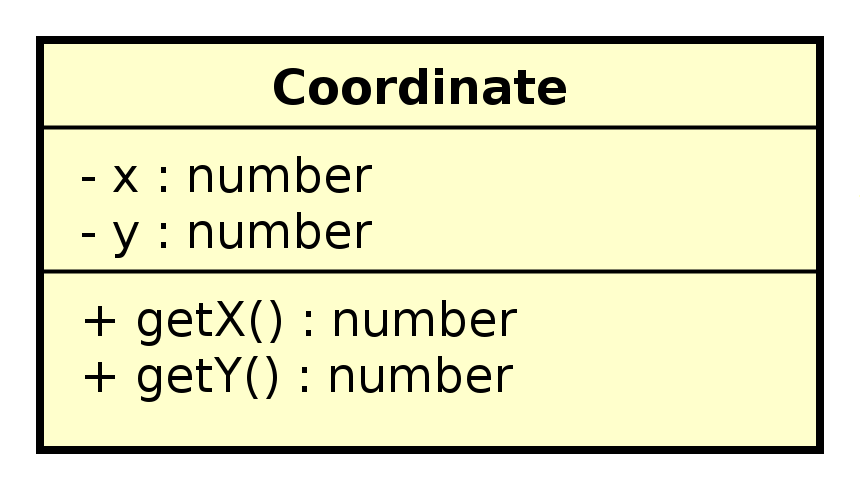
\includegraphics[width=0.3\textwidth]{./img/Coordinate.png}
		\caption{Diagramma classe Coordinate}
	\end{figure}
	\item \textbf{descrizione:} rappresenta una coordinata geografica;
	\item \textbf{utilizzo:} è utilizzata all'interno di Polygon per delimitarne i suoi vertici;
	\item \textbf{attributi:}
	\begin{itemize}
		\item -x : number\begin{itemize}
			\item rappresenta la latitudine di una coordinata geografica.\end{itemize}
		\item -y : number\begin{itemize}
			\item rappresenta la longitudine di una coordinata geografica.\end{itemize}
	\end{itemize}
	\item \textbf{metodi:}
	\begin{itemize}
		\item +getX() : number\newline
		restituisce la latitudine della coordinata geografica
		\item +getY() : number\newline
		restituisce la longitudine della coordinata geografica
	\end{itemize}
\end{itemize}
\paragraph{Polygon}
\begin{itemize}
	\begin{figure}[H]
		\centering
		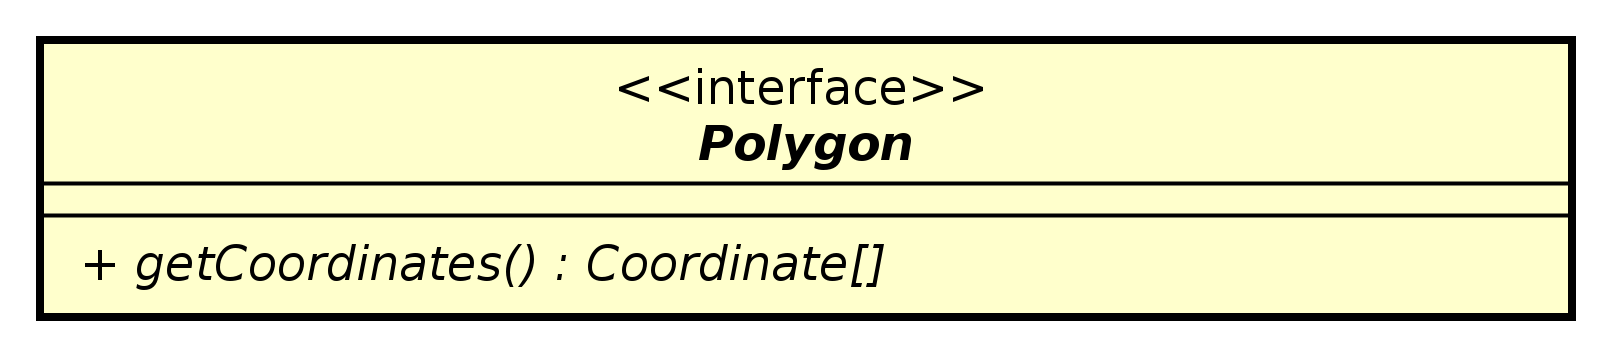
\includegraphics[width=0.3\textwidth]{./img/Polygon.png}
		\caption{Diagramma classe Polygon}
	\end{figure}
	\item \textbf{descrizione:} interfaccia che rappresenta il poligono;
	\item \textbf{utilizzo:} fornisce i metodi del poligono;
	\item \textbf{metodi:}
	\begin{itemize}
		\item +getCoordinates() : Coordinate[]\newline
		il metodo restituisce un array di coordinate
	\end{itemize}
\end{itemize}
\paragraph{PolygonFactory}
\begin{itemize}
	\begin{figure}[H]
		\centering
		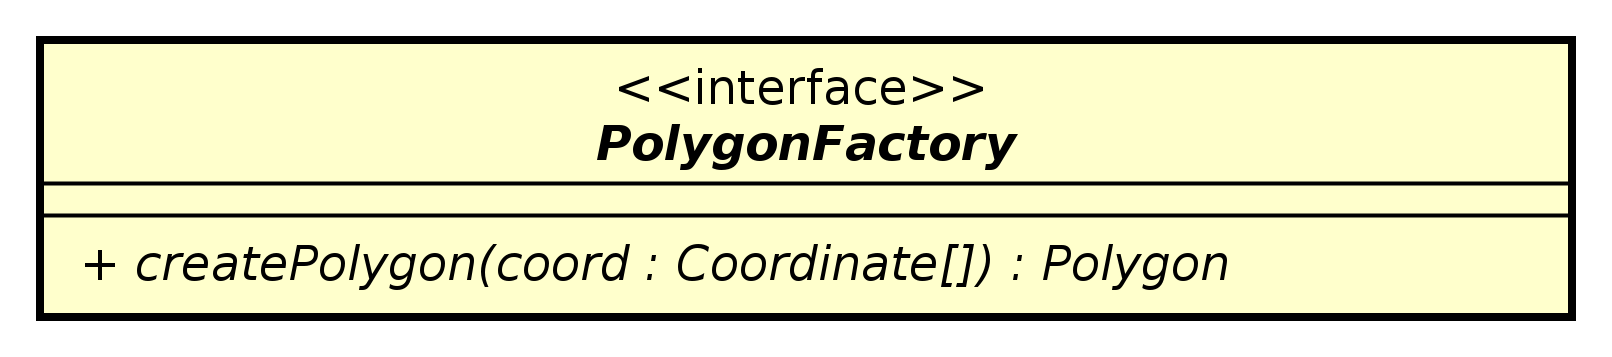
\includegraphics[width=0.3\textwidth]{./img/PolygonFactory.png}
		\caption{Diagramma classe PolygonFactory}
	\end{figure}
	\item \textbf{descrizione:} interfaccia che si occupa della costruzione dei poligoni;
	\item \textbf{utilizzo:} viene usata dalle classi Scenario e Asset per la costruzione dei poligoni;
	\item \textbf{metodi:}
	\begin{itemize}
		\item +createPolygon(coord) : Polygon\newline
		il metodo si occupa della costruzione del poligono
		\begin{itemize}
			\item coord : Coordinate[]\\
			raccoglie le coordinate necessarie alla costruzione dei poligoni
			.
		\end{itemize}
	\end{itemize}
\end{itemize}
\newpage
\subsection{DeGeOP::ReducerPkg}
\label{pkg::ReducerPkg}
\begin{figure}[H]
	\centering
	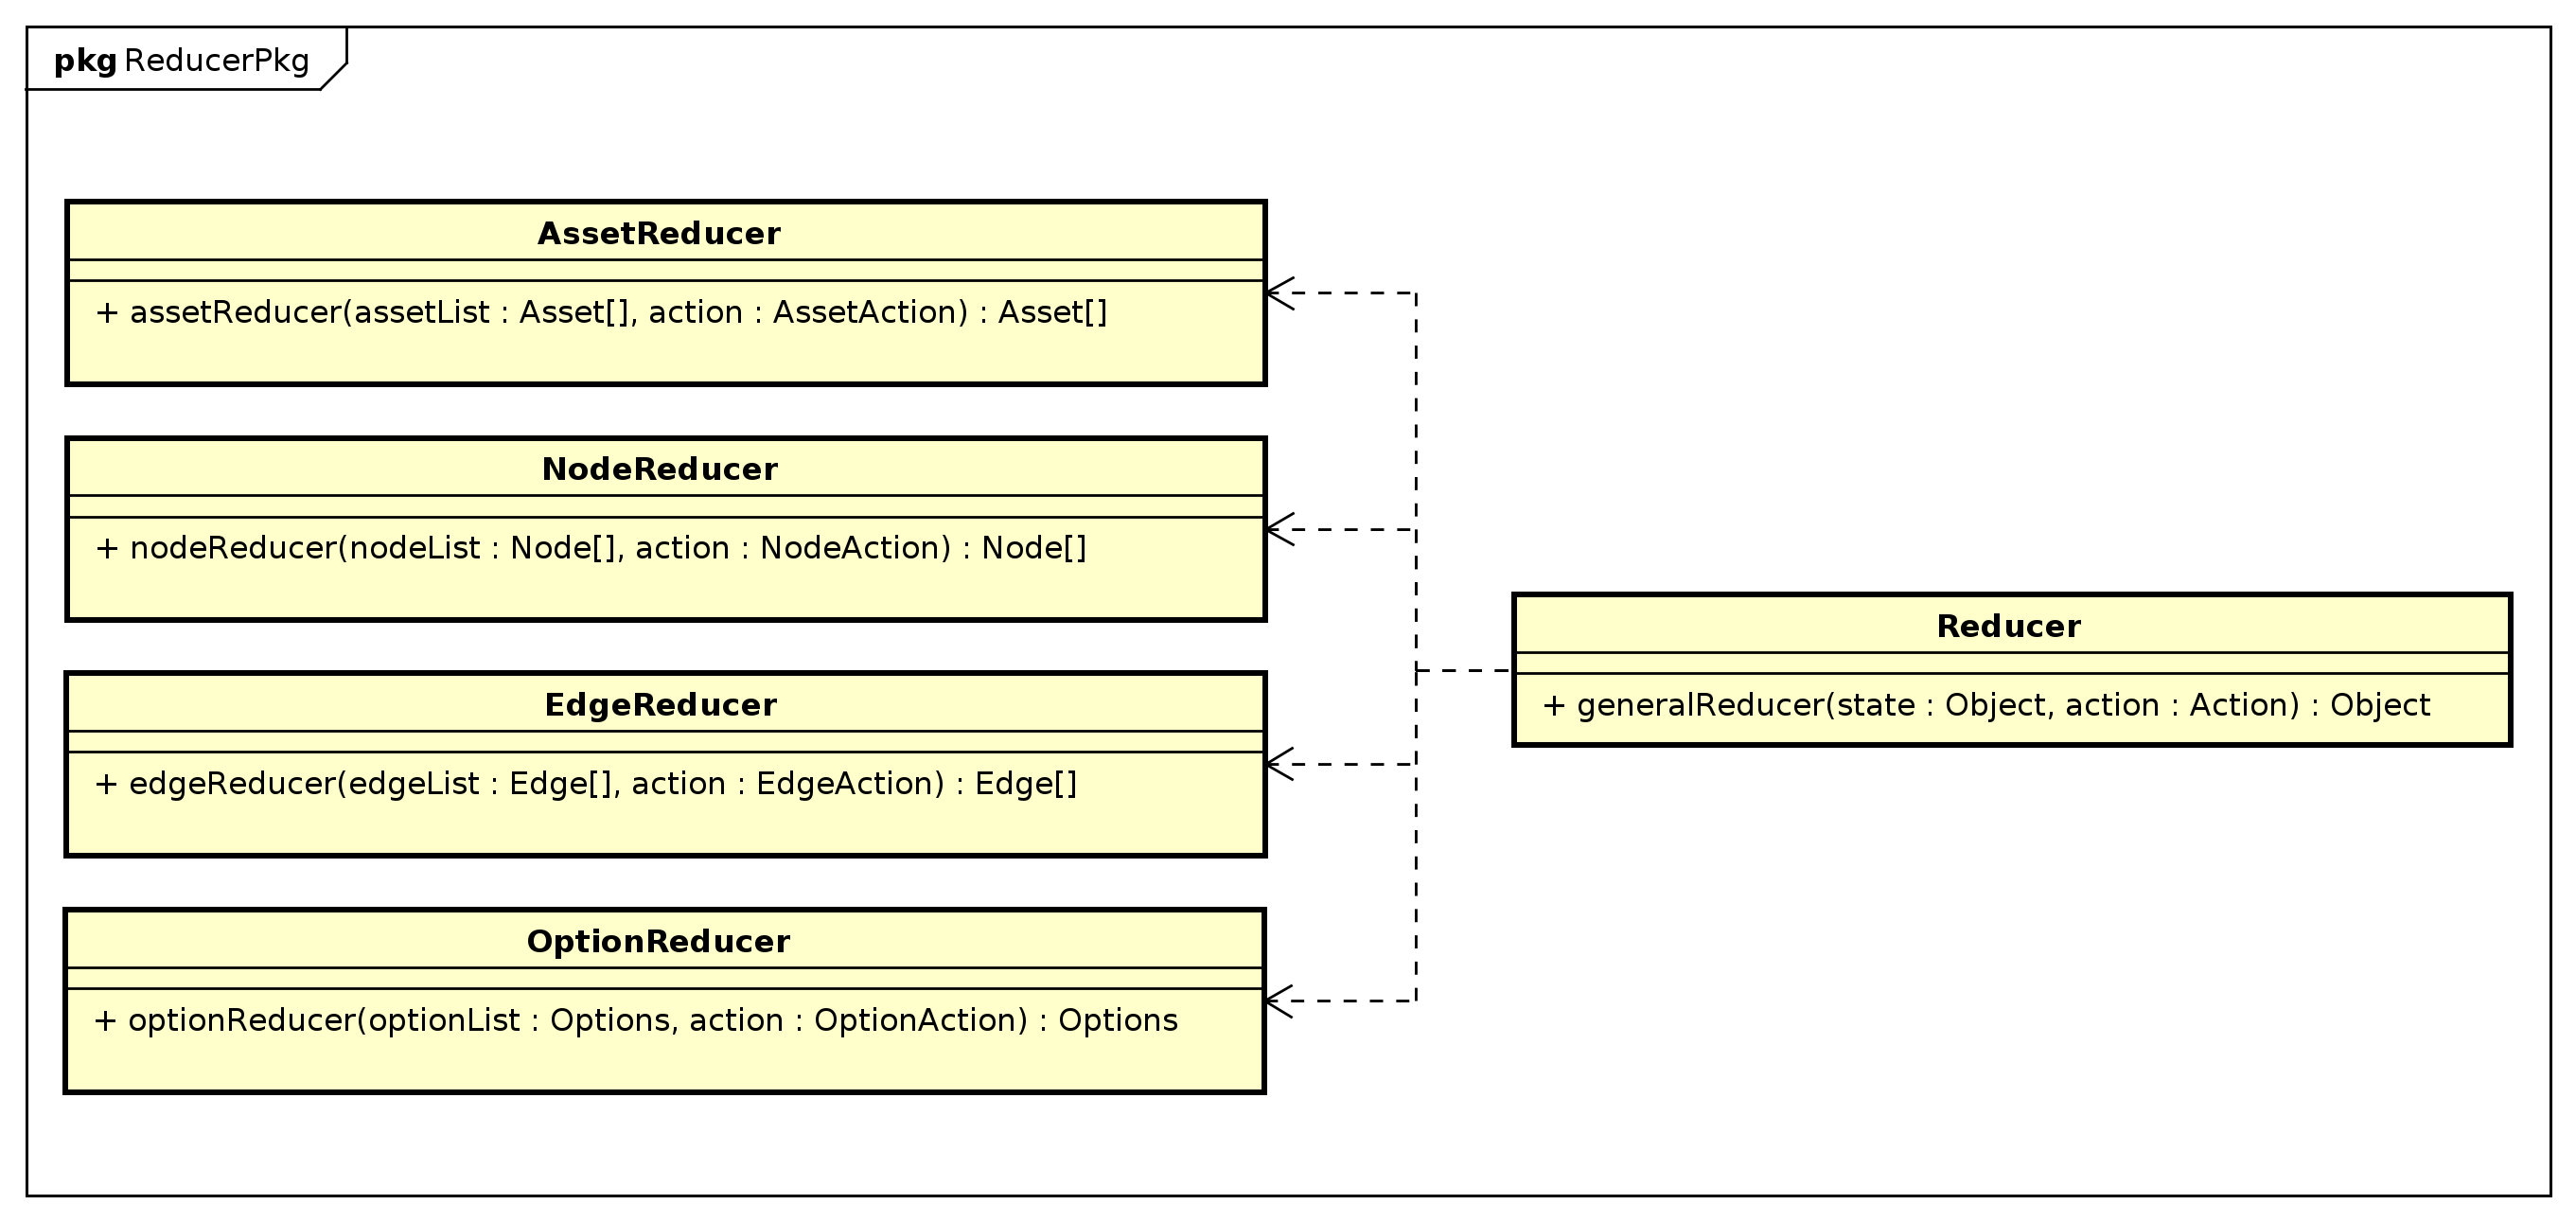
\includegraphics[width=\textwidth]{img/PkgDiagram/ReducerPkg.png}
	\caption{Schema componente DeGeOP::ReducerPkg}
\end{figure}
\subsubsection{Informazioni sul package}
\begin{itemize}
	\item \textbf{descrizione:} racchiude le componenti necessarie all'implementazione dei reducer secondo l'architettura Redux;
	\item \textbf{padre:} \hyperref[pkg::DeGeOP]{DeGeOP};
	\item \textbf{interazioni con altri package:} 
	\begin{itemize}
		\item OUT ActionPkg: utilizzo di azioni ;
		\item OUT StorePkg: applicazione di cambiamenti di stato.
	\end{itemize}
	\item \textbf{classi contenute:}
	\begin{itemize}
		\item AssetReducer;
		\item EdgeReducer;
		\item NodeReducer;
		\item OptionReducer;
		\item Reducer.
	\end{itemize}
\end{itemize}
\subsubsection{Classi}
\paragraph{AssetReducer}
\begin{itemize}
	\begin{figure}[H]
		\centering
		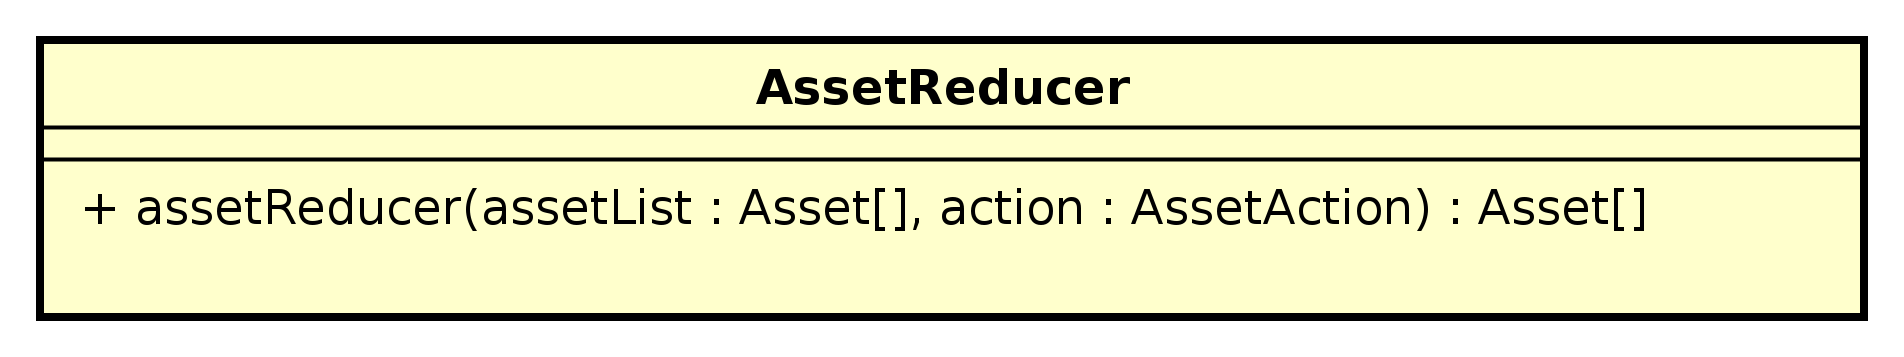
\includegraphics[width=0.3\textwidth]{./img/AssetReducer.png}
		\caption{Diagramma classe AssetReducer}
	\end{figure}
	\item \textbf{descrizione:} rappresenta il reducer dell'asset;
	\item \textbf{utilizzo:} il suo metodo gestisce le operazioni sullo store riguardanti l'asset;
	\item \textbf{metodi:}
	\begin{itemize}
		\item +assetReducer(action, assetList) : Asset[ ]\newline
		il metodo gestisce le operazioni sullo store riguardanti l'asset e ritorna la nuova lista di asset ottenuta a seguito della modifica
		\begin{itemize}
			\item action : AssetAction\\
			rappresenta un'azione che descrive i cambiamenti da effettuare sullo stato.
			\item assetList : Asset[ ]\\
			rappresenta una lista di asset, che sono il vecchio stato.
		\end{itemize}
	\end{itemize}
	\item \textbf{relazioni con altre classi:} 
	\begin{itemize}
		\item OUT Asset.
	\end{itemize}
\end{itemize}
\paragraph{EdgeReducer}
\begin{itemize}
	\begin{figure}[H]
		\centering
		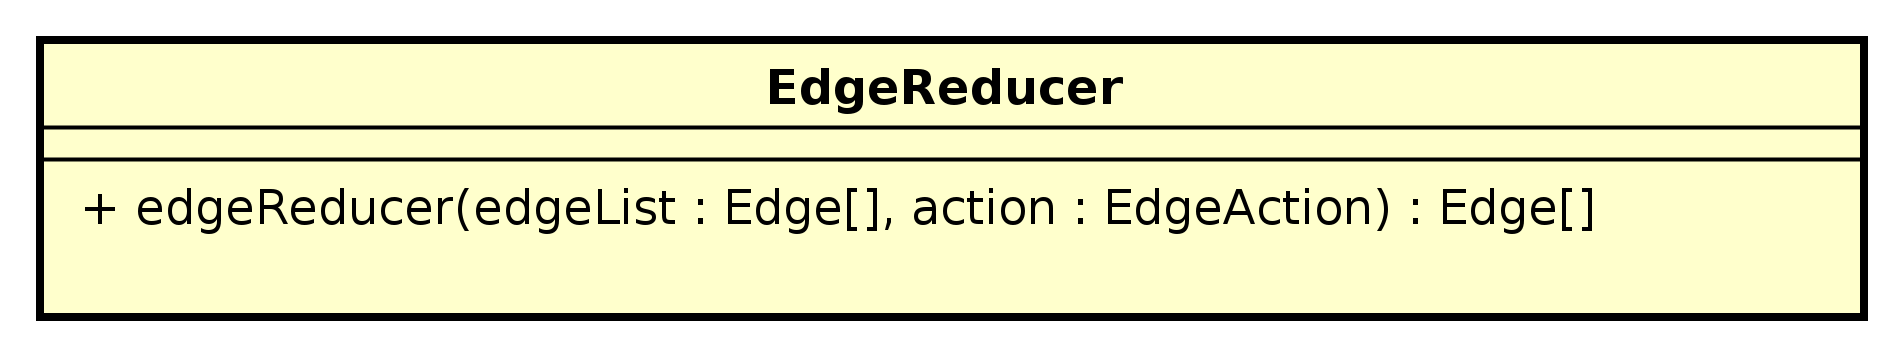
\includegraphics[width=0.3\textwidth]{./img/EdgeReducer.png}
		\caption{Diagramma classe EdgeReducer}
	\end{figure}
	\item \textbf{descrizione:} rappresenta il reducer dell'arco;
	\item \textbf{utilizzo:} il suo metodo gestisce le operazioni sullo store riguardanti gli archi;
	\item \textbf{metodi:}
	\begin{itemize}
		\item +edgeReducer(action, edgeList) : Edge [ ]\newline
		il metodo gestisce le operazioni sullo store riguardanti gli archi e ritorna la nuova lista di archi ottenuta a seguito della modifica
		\begin{itemize}
			\item action : EdgeAction\\
			rappresenta un'azione che descrive i cambiamenti da effettuare sullo stato.
			\item edgeList : Edge [ ]\\
			rappresenta una lista di archi, che sono il vecchio stato.
		\end{itemize}
	\end{itemize}
	\item \textbf{relazioni con altre classi:} 
	\begin{itemize}
		\item OUT Edge.
	\end{itemize}
\end{itemize}
\paragraph{NodeReducer}
\begin{itemize}
	\begin{figure}[H]
		\centering
		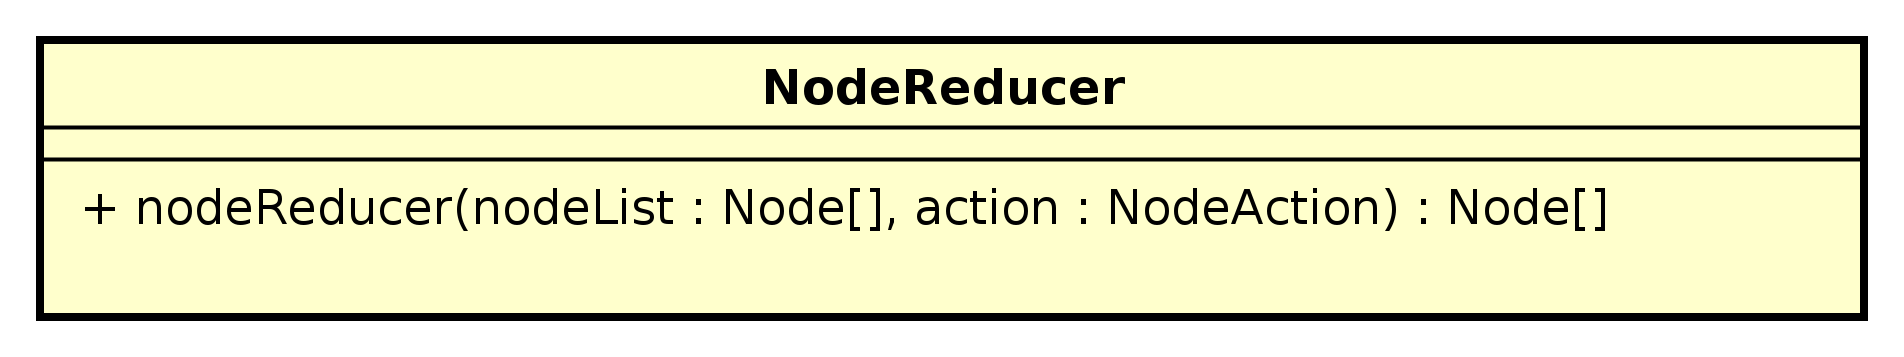
\includegraphics[width=0.3\textwidth]{./img/NodeReducer.png}
		\caption{Diagramma classe NodeReducer}
	\end{figure}
	\item \textbf{descrizione:} rappresenta il reducer del nodo;
	\item \textbf{utilizzo:} il suo metodo gestisce le operazioni sullo store riguardanti i nodi;
	\item \textbf{metodi:}
	\begin{itemize}
		\item +nodeReducer(action, nodeList) : Node [ ]\newline
		il metodo gestisce le operazioni sullo store riguardanti i nodi e ritorna la nuova lista di nodi ottenuta a seguito della modifica
		\begin{itemize}
			\item action : EdgeAction\\
			rappresenta un'azione che descrive i cambiamenti da effettuare sullo stato.
			\item nodeList : Node [ ]\\
			rappresenta una lista di nodi, che sono il vecchio stato.
		\end{itemize}
	\end{itemize}
	\item \textbf{relazioni con altre classi:} 
	\begin{itemize}
		\item OUT Node.
	\end{itemize}
\end{itemize}
\paragraph{OptionReducer}
\begin{itemize}
	\begin{figure}[H]
		\centering
		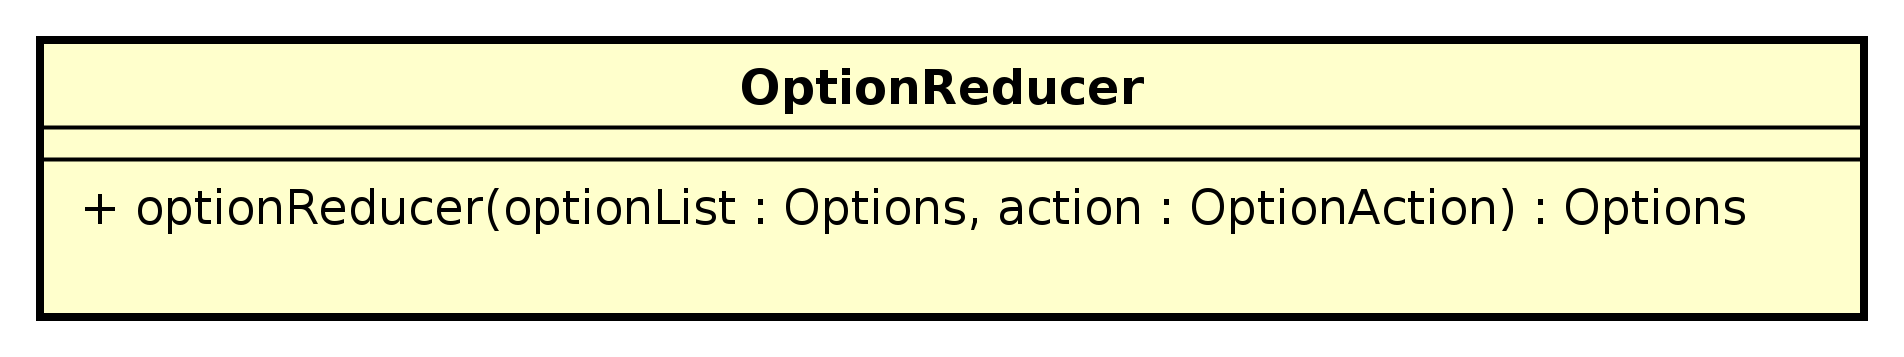
\includegraphics[width=0.3\textwidth]{./img/OptionReducer.png}
		\caption{Diagramma classe OptionReducer}
	\end{figure}
	\item \textbf{descrizione:} rappresenta il reducer delle option;
	\item \textbf{utilizzo:} il suo metodo gestisce le operazioni sullo store riguardanti l'asset;
	\item \textbf{metodi:}
	\begin{itemize}
		\item +optionReducer(action, optionList) : Options\newline
		il metodo gestisce le operazioni sullo store riguardanti l'asset e ritorna la nuova lista di asset ottenuta a seguito della modifica
		\begin{itemize}
			\item action : OptionAction\\
			rappresenta un'azione che descrive i cambiamenti da effettuare sullo stato.
			\item optionList : Options\\
			rappresenta la lista delle option.
		\end{itemize}
	\end{itemize}
	\item \textbf{relazioni con altre classi:} 
	\begin{itemize}
		\item IN Reducer;
		\item OUT Options.
	\end{itemize}
\end{itemize}
\paragraph{Reducer}
\begin{itemize}
	\begin{figure}[H]
		\centering
		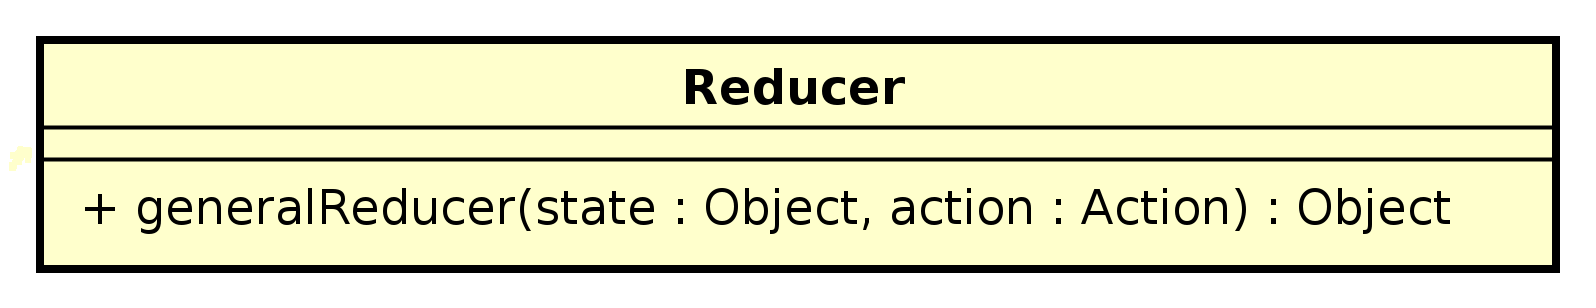
\includegraphics[width=0.3\textwidth]{./img/Reducer.png}
		\caption{Diagramma classe Reducer}
	\end{figure}
	\item \textbf{descrizione:} accetta una action generica in input e la reindirizza al giusto reducer;
	\item \textbf{utilizzo:} il suo metodo viene utilizzato per catturare un'azione e generare un nuovo stato sullo Store;
	\item \textbf{metodi:}
	\begin{itemize}
		\item +generalReducer() : Object\newline
		Esegue l'azione sullo stato corrente dello store e ne ritorna il nuovo stato
	\end{itemize}
	\item \textbf{relazioni con altre classi:} 
	\begin{itemize}
		\item OUT OptionReducer;
		\item OUT StoreDeGeOP.
	\end{itemize}
\end{itemize}
\newpage
\subsection{DeGeOP::CallManagerPkg}
\label{pkg::CallManagerPkg}
\begin{figure}[H]
	\centering
	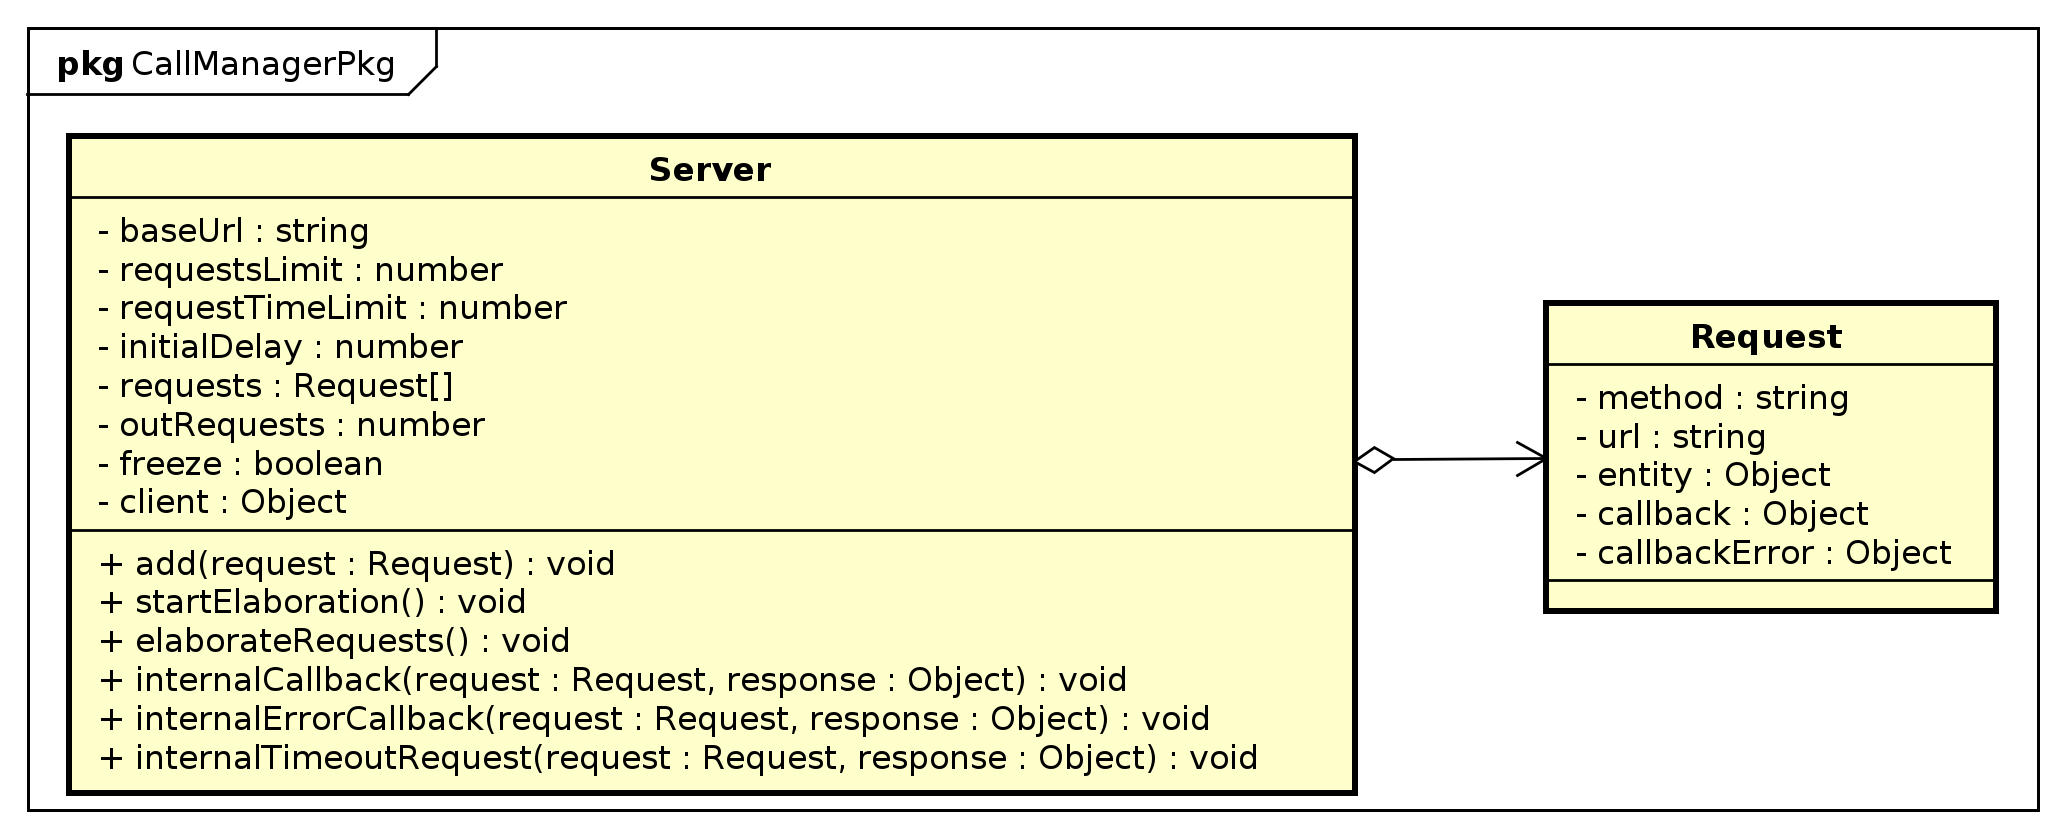
\includegraphics[width=\textwidth]{img/PkgDiagram/CallManagerPkg.png}
	\caption{Schema componente DeGeOP::CallManagerPkg}
\end{figure}
\subsubsection{Informazioni sul package}
\begin{itemize}
	\item \textbf{descrizione:} racchiude le componenti necessarie alla comunicazione dei dati verso il server;
	\item \textbf{padre:} \hyperref[pkg::DeGeOP]{DeGeOP};
	\item \textbf{interazioni con altri package:} 
	\begin{itemize}
		\item OUT ActionPkg: dispatch di azioni;
		\item OUT StorePkg: subscribe sullo store.
	\end{itemize}
	\item \textbf{classi contenute:}
	\begin{itemize}
		\item Request;
		\item Server.
	\end{itemize}
\end{itemize}
\subsubsection{Classi}
\paragraph{Request}
\begin{itemize}
	\begin{figure}[H]
		\centering
		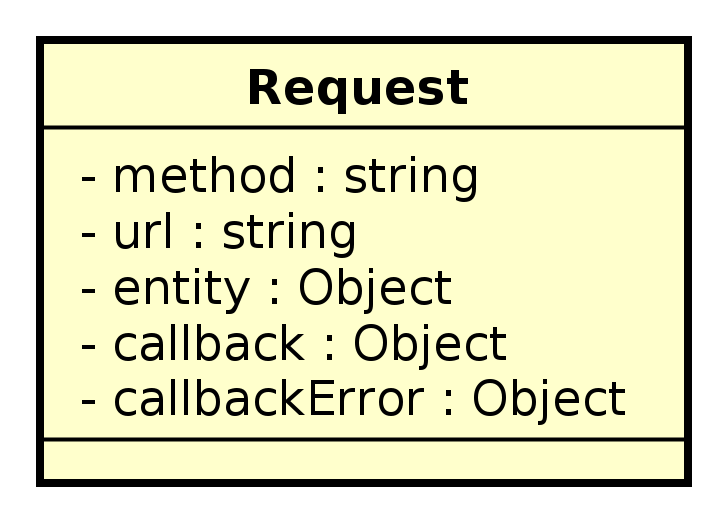
\includegraphics[width=0.3\textwidth]{./img/Request.png}
		\caption{Diagramma classe Request}
	\end{figure}
	\item \textbf{descrizione:} rappresenta i dati necessari per eseguire una richiesta di tipologia REST;
	\item \textbf{utilizzo:} è utilizzata all'interno di Server per gestire la coda delle richieste ;
	\item \textbf{attributi:}
	\begin{itemize}
		\item -callback : Object\begin{itemize}
			\item rappresenta la funzione che viene invocata se la richiesta è andata a buon fine.\end{itemize}
		\item -callbackError : Object\begin{itemize}
			\item rappresenta la funzione che viene invocata se la richiesta non è andata a buon fine.\end{itemize}
		\item -entity : Object\begin{itemize}
			\item rappresnta il payload della richiesta.\end{itemize}
		\item -method : string\begin{itemize}
			\item rappresenta il verbo http con cui si esegue la richiesta.\end{itemize}
		\item -url : string\begin{itemize}
			\item rappresenta l'url verso cui eseguire la richiesta.\end{itemize}
	\end{itemize}
\end{itemize}
\paragraph{Server}
\begin{itemize}
	\begin{figure}[H]
		\centering
		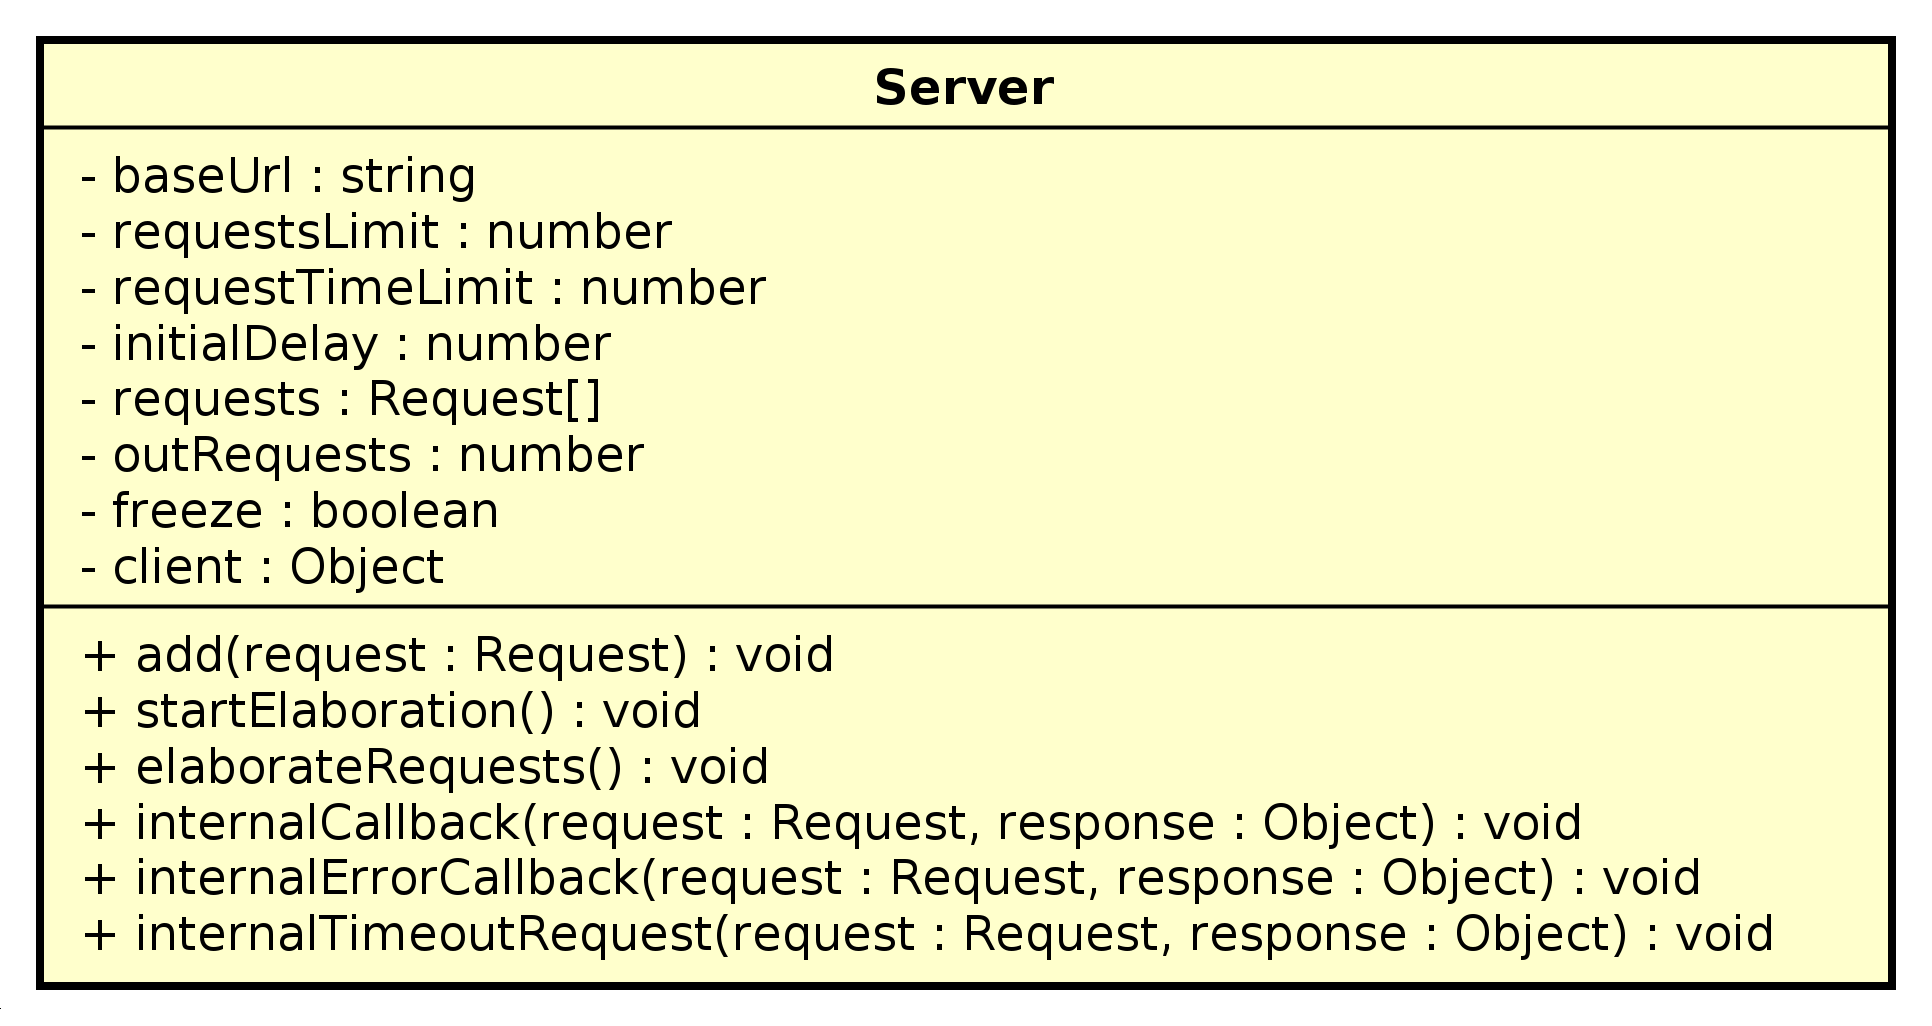
\includegraphics[width=0.3\textwidth]{./img/Server.png}
		\caption{Diagramma classe Server}
	\end{figure}
	\item \textbf{descrizione:} rappresenta il gestore delle chiamate REST;
	\item \textbf{utilizzo:} è utilizzato come buffer per gestire le richieste in uscita e le risposte ricevute;
	\item \textbf{attributi:}
	\begin{itemize}
		\item -baseUrl : string\begin{itemize}
			\item URL http verso cui devono essere inviate le richieste.\end{itemize}
		\item -client : Object\begin{itemize}
			\item gestisce l'invio delle richieste e la ricezione delle risposte.\end{itemize}
		\item -freeze : boolean\begin{itemize}
			\item viene utilizzata per bloccare il server in caso di collegamento mancante.\end{itemize}
		\item -initialDelay : number\begin{itemize}
			\item rappresenta il tempo in millisecondi passato il quale una richiesta scaduta viene eseguita nuovamente.\end{itemize}
		\item -outRequests : number\begin{itemize}
			\item rappresenta il numero delle richieste attualmente in attesa di risposta.\end{itemize}
		\item -requests : Request[]\begin{itemize}
			\item lista delle richieste da evadere.\end{itemize}
		\item -requestsLimit : number\begin{itemize}
			\item rappresenta il numero massimo di richieste eseguite ancora in attesa di risposta.\end{itemize}
		\item -timeLimitRequest : number\begin{itemize}
			\item rappresenta il tempo in millisecondi dopo cui considerare la richiesta scaduta.\end{itemize}
	\end{itemize}
	\item \textbf{metodi:}
	\begin{itemize}
		\item +add(request) : void\newline
		aggiunge una richiesta alla coda del server
		\begin{itemize}
			\item request : Request\\
			rappresenta la richiesta da aggiungere alla coda server.
		\end{itemize}
		\item +elaborateRequests() : void\newline
		elabora la coda della richieste fino a quando ci sono elementi presenti
		\item +internalCallback(request, response) : void\newline
		esegue la chiamata alla funzione di callback fornita dalla richiesta nel caso in cui questa abbia ricevuto una risposta senza errori
		\begin{itemize}
			\item request : Request\\
			rappresenta la richiesta che è stata inviata.
			\item response : Object\\
			oggetto che rappresenta la risposta alla richiesta inviata.
		\end{itemize}
		\item +internalErrorCallback(request, response) : void\newline
		esegue la chiamata alla funzione di callback fornita dalla richiesta nel caso in cui questa abbia ricevuto una risposta con errori
		\begin{itemize}
			\item request : Request\\
			rappresenta la richiesta che è stata inviata.
			\item response : Object\\
			oggetto che rappresenta la risposta alla richiesta inviata.
		\end{itemize}
		\item +internalTimeoutRequest(response) : void\newline
		gestisce la richiesta nel caso in cui questa abbia non abbia ricevuto alcuna risposta entro il tempo di timeout
		\begin{itemize}
			\item response : Object\\
			oggetto che rappresenta la risposta alla richiesta inviata.
		\end{itemize}
		\item +startElaboration() : void\newline
		inizia l'esecuzione delle richieste in attesa di essere evase
	\end{itemize}
\end{itemize}
\newpage
\subsection{DeGeOP::ActionPkg}
\label{pkg::ActionPkg}
\begin{figure}[H]
	\centering
	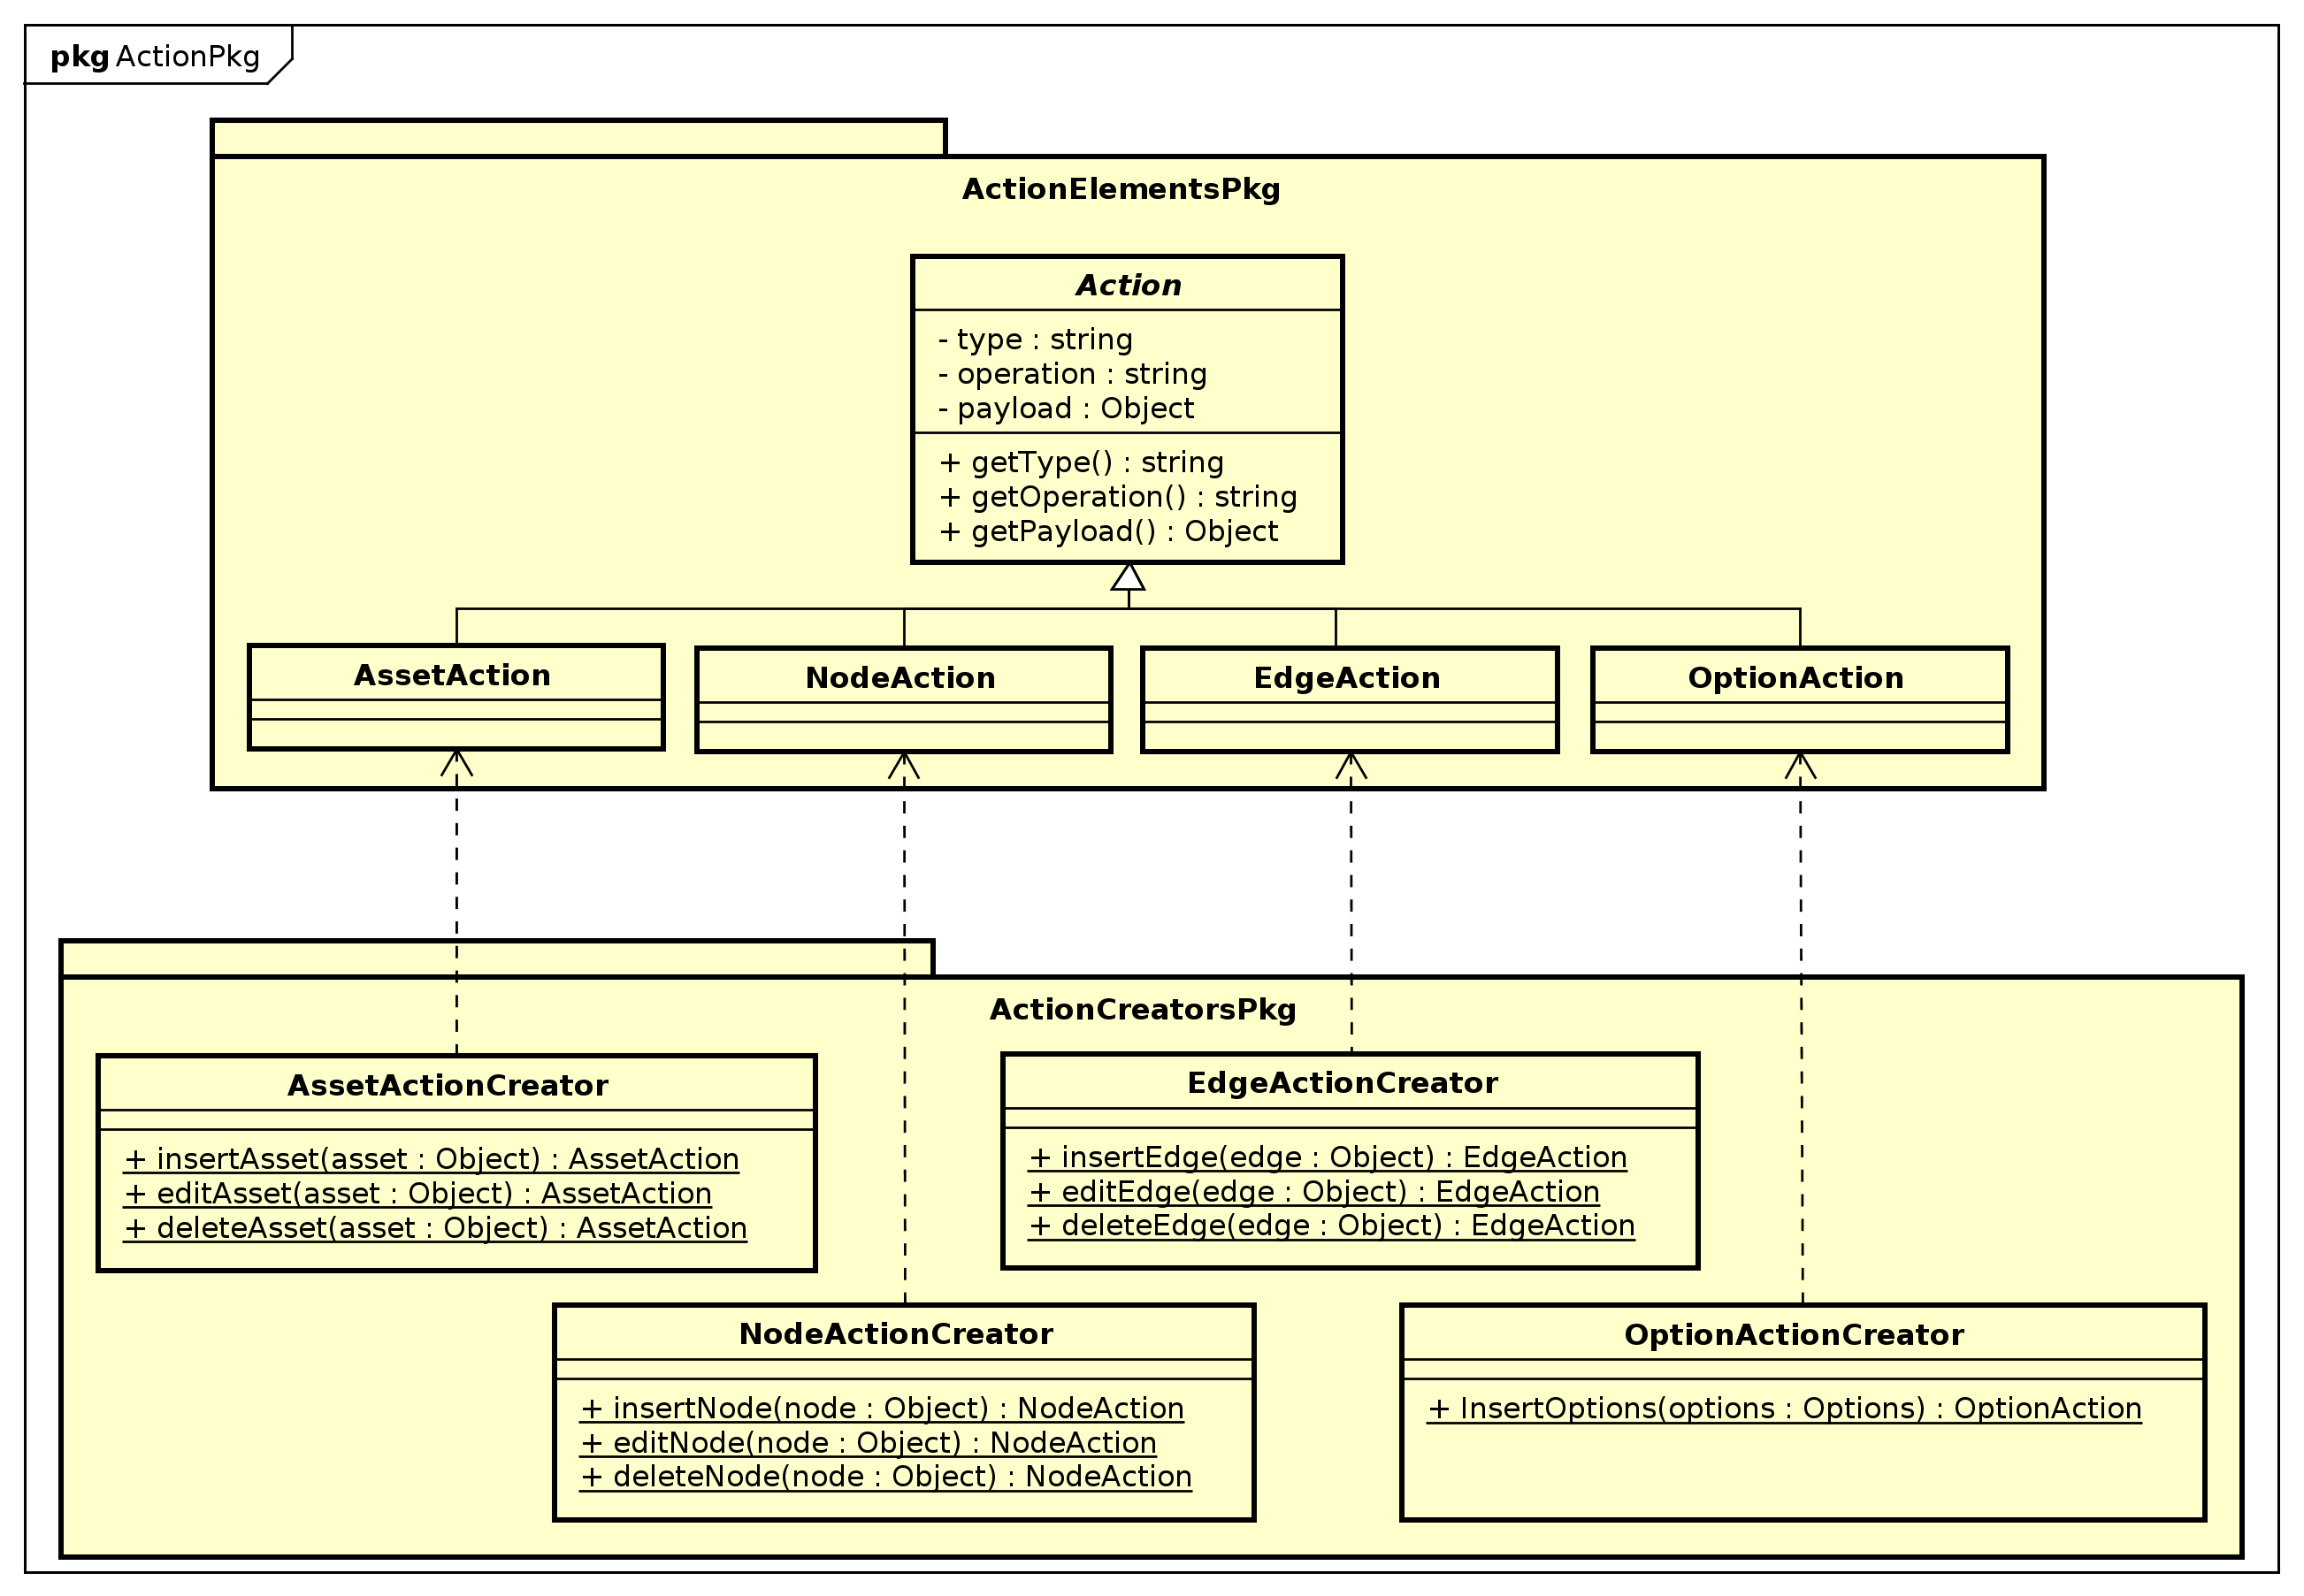
\includegraphics[width=\textwidth]{img/PkgDiagram/ActionPkg.png}
	\caption{Schema componente DeGeOP::ActionPkg}
\end{figure}
\subsubsection{Informazioni sul package}
\begin{itemize}
	\item \textbf{descrizione:} racchiude le componenti utilizzate per implementare le action dell'architettura Redux. Le action vengono create e ne viene fatto il dispatch verso lo store. Un reducer gestirà una action per produrre un cambiamento di stato sullo store;
	\item \textbf{padre:} \hyperref[pkg::DeGeOP]{DeGeOP};
	\item \textbf{package contenuti:}
	\begin{itemize}
		\item ActionPkg::\hyperref[pkg::ActionCreatorsPkg]{ActionCreatorsPkg};
		\item ActionPkg::\hyperref[pkg::ActionElementsPkg]{ActionElementsPkg}.
	\end{itemize}
	\item \textbf{interazioni con altri package:} 
	\begin{itemize}
		\item IN CallManagerPkg: dispatch di azioni;
		\item IN ReducerPkg: utilizzo di azioni ;
		\item IN ViewPkg: dispatch di azioni.
	\end{itemize}
	\item \textbf{classi contenute:}
	\begin{itemize}
		\item EdgeAction.
	\end{itemize}
\end{itemize}
\subsubsection{Classi}
\paragraph{EdgeAction}
\begin{itemize}
	\begin{figure}[H]
		\centering
		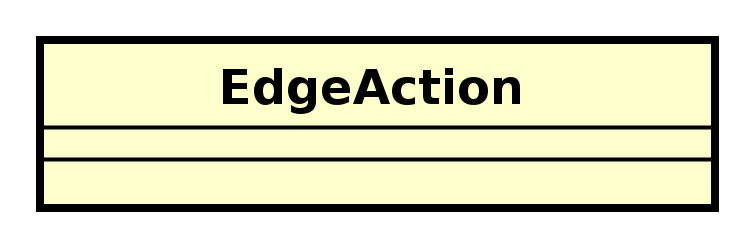
\includegraphics[width=0.3\textwidth]{./img/EdgeAction.png}
		\caption{Diagramma classe EdgeAction}
	\end{figure}
	\item \textbf{descrizione:} rappresenta un'azione relativa agli archi;
	\item \textbf{utilizzo:} l'azione viene creata da un apposito ActionCreator per essere poi inviata ad un reducer.
\end{itemize}
\newpage
\subsection{DeGeOP::ActionPkg::ActionElementsPkg}
\label{pkg::ActionElementsPkg}
\subsubsection{Informazioni sul package}
\begin{itemize}
	\item \textbf{descrizione:} racchiude le componenti che rappresentano effettivamente le azioni;
	\item \textbf{padre:} \hyperref[pkg::ActionPkg]{ActionPkg};
	\item \textbf{interazioni con altri package:} 
	\begin{itemize}
		\item IN ActionCreatorsPkg: creazione di azioni.
	\end{itemize}
	\item \textbf{classi contenute:}
	\begin{itemize}
		\item Action;
		\item AssetAction;
		\item NodeAction;
		\item OptionAction.
	\end{itemize}
\end{itemize}
\subsubsection{Classi}
\paragraph{Action}
\begin{itemize}
	\begin{figure}[H]
		\centering
		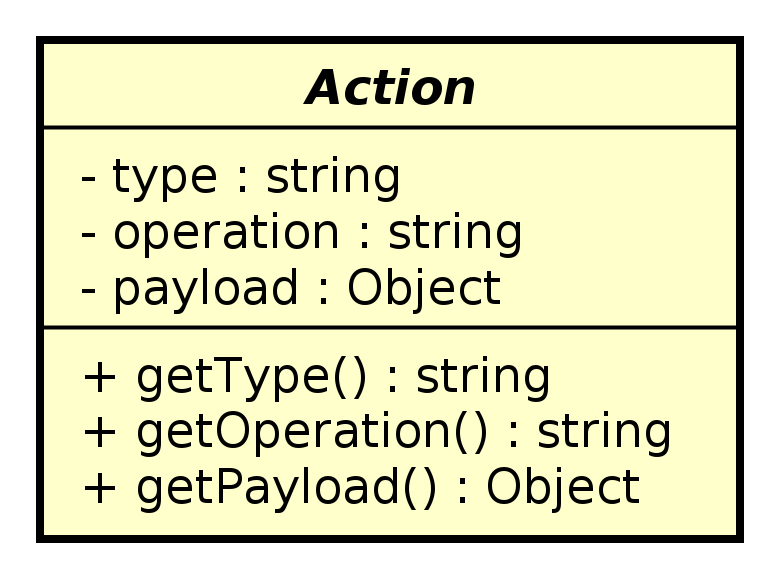
\includegraphics[width=0.3\textwidth]{./img/Action.png}
		\caption{Diagramma classe Action}
	\end{figure}
	\item \textbf{descrizione:} una classe astratta che rappresenta una generica azione di cui può essere fatto il dispatch;
	\item \textbf{utilizzo:} i suoi membri vengono usati dai reducer per completare una azione;
	\item \textbf{attributi:}
	\begin{itemize}
		\item -operation : string\begin{itemize}
			\item rappresenta l'operazione da eseguire.\end{itemize}
		\item -payload : Object\begin{itemize}
			\item rappresenta l'oggetto che descrive il cambiamento apportato dall'azione.\end{itemize}
		\item -type : string\begin{itemize}
			\item rappresenta la tipologia di elemento su cui eseguire l'azione.\end{itemize}
	\end{itemize}
	\item \textbf{metodi:}
	\begin{itemize}
		\item +getOperation() : string\newline
		il metodo ritorna l'operazione eseguita dall'azione
		\item +getPayload() : Object\newline
		il metodo ritorna il payload dell'oggetto
		\item +getType() : string\newline
		il metodo ritorna il tipo dell'azione
	\end{itemize}
\end{itemize}
\paragraph{AssetAction}
\begin{itemize}
	\begin{figure}[H]
		\centering
		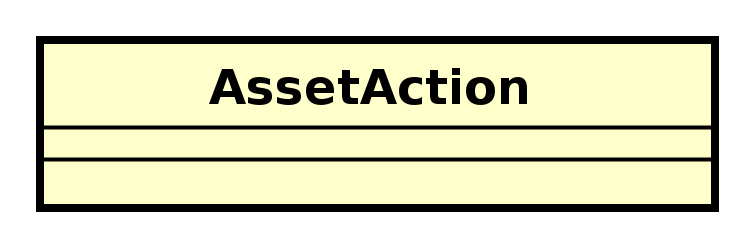
\includegraphics[width=0.3\textwidth]{./img/AssetAction.png}
		\caption{Diagramma classe AssetAction}
	\end{figure}
	\item \textbf{descrizione:} rappresenta un'azione relativa agli asset;
	\item \textbf{utilizzo:} l'azione viene creata da un apposito ActionCreator per essere poi inviata ad un reducer.
\end{itemize}
\paragraph{NodeAction}
\begin{itemize}
	\begin{figure}[H]
		\centering
		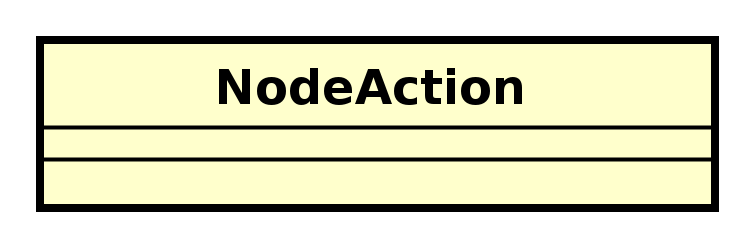
\includegraphics[width=0.3\textwidth]{./img/NodeAction.png}
		\caption{Diagramma classe NodeAction}
	\end{figure}
	\item \textbf{descrizione:} rappresenta un'azione relativa ai nodi;
	\item \textbf{utilizzo:} l'azione viene creata da un apposito ActionCreator per essere poi inviata ad un reducer.
\end{itemize}
\paragraph{OptionAction}
\begin{itemize}
	\begin{figure}[H]
		\centering
		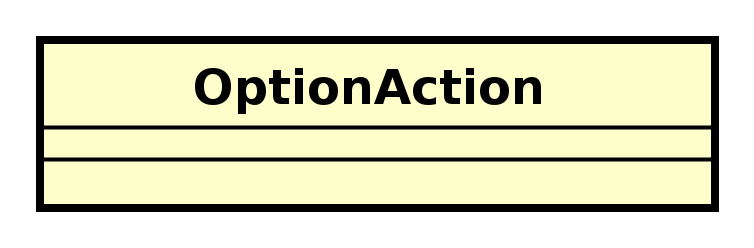
\includegraphics[width=0.3\textwidth]{./img/OptionAction.png}
		\caption{Diagramma classe OptionAction}
	\end{figure}
	\item \textbf{descrizione:} rappresenta un'azione relativa all'oggetto option;
	\item \textbf{utilizzo:} l'azione viene creata da un apposito ActionCreator per essere poi inviata ad un reducer;
	\item \textbf{relazioni con altre classi:} 
	\begin{itemize}
		\item IN OptionActionCreator.
	\end{itemize}
\end{itemize}
\newpage
\subsection{DeGeOP::ActionPkg::ActionCreatorsPkg}
\label{pkg::ActionCreatorsPkg}
\subsubsection{Informazioni sul package}
\begin{itemize}
	\item \textbf{descrizione:} racchiude le componenti che gestiscono la creazione delle azioni;
	\item \textbf{padre:} \hyperref[pkg::ActionPkg]{ActionPkg};
	\item \textbf{interazioni con altri package:} 
	\begin{itemize}
		\item OUT ActionElementsPkg: creazione di azioni.
	\end{itemize}
	\item \textbf{classi contenute:}
	\begin{itemize}
		\item AssetActionCreator;
		\item EdgeActionCreator;
		\item NodeActionCreator;
		\item OptionActionCreator.
	\end{itemize}
\end{itemize}
\subsubsection{Classi}
\paragraph{AssetActionCreator}
\begin{itemize}
	\begin{figure}[H]
		\centering
		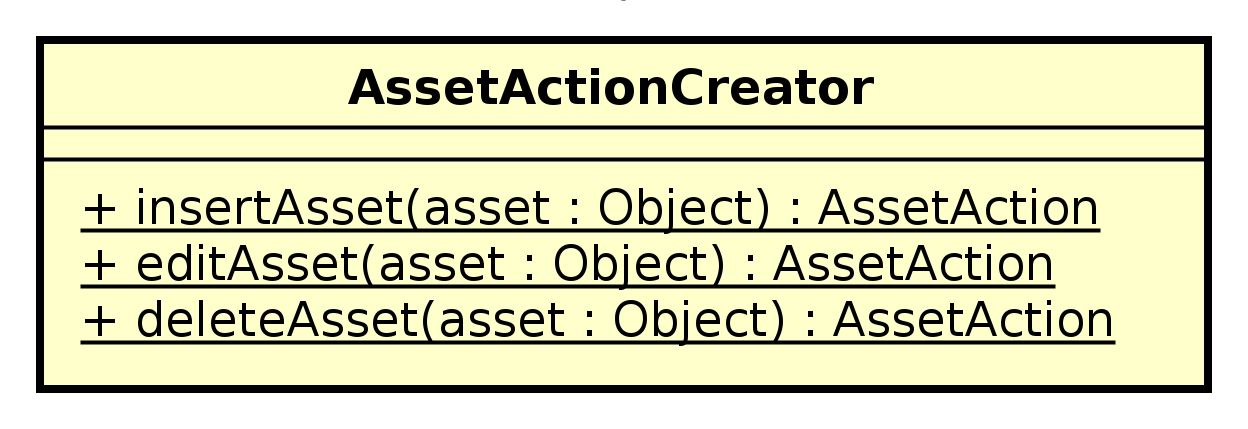
\includegraphics[width=0.3\textwidth]{./img/AssetActionCreator.png}
		\caption{Diagramma classe AssetActionCreator}
	\end{figure}
	\item \textbf{descrizione:} rappresenta la factory di azioni relative agli asset;
	\item \textbf{utilizzo:} i suoi metodi sono chiamati dalla View e dal CallManager per la creazione di azioni relative agli asset;
	\item \textbf{metodi:}
	\begin{itemize}
		\item +deleteAsset(asset) : AssetAction\newline
		il metodo crea l'azione relativa all'eliminazione dell'asset ricevuto in input
		\begin{itemize}
			\item asset : Object\\
			oggetto contenente i parametri di un Asset che dovrà essere eliminato.
		\end{itemize}
		\item +editAsset(asset) : AssetAction\newline
		il metodo crea l'azione relativa alla modifica di un asset
		\begin{itemize}
			\item asset : Object\\
			oggetto contenente i parametri di un Asset che dovrà essere modificato nello store.
		\end{itemize}
		\item +insertAsset(asset) : AssetAction\newline
		il metodo crea l'azione relativa all'inserimento di un nuovo asset
		\begin{itemize}
			\item asset : Object\\
			oggetto contenente i parametri di un Asset che dovrà essere inserito nello store.
		\end{itemize}
	\end{itemize}
\end{itemize}
\paragraph{EdgeActionCreator}
\begin{itemize}
	\begin{figure}[H]
		\centering
		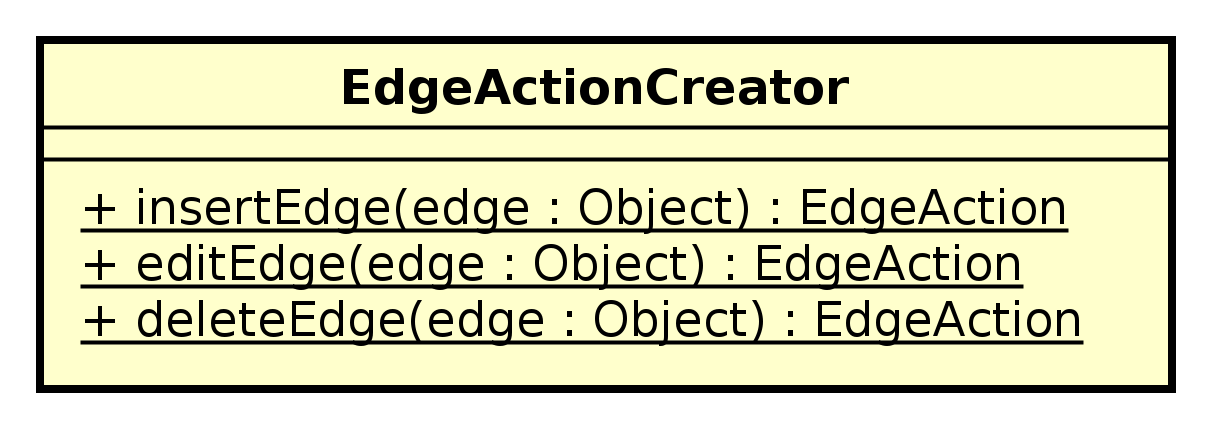
\includegraphics[width=0.3\textwidth]{./img/EdgeActionCreator.png}
		\caption{Diagramma classe EdgeActionCreator}
	\end{figure}
	\item \textbf{descrizione:} rappresenta la factory di azioni relative agli archi;
	\item \textbf{utilizzo:} i suoi metodi sono chiamati dalla View e dal CallManager per la creazione di azioni relative agli archi;
	\item \textbf{metodi:}
	\begin{itemize}
		\item +deleteEdge(edge) : EdgeAction\newline
		il metodo crea l'azione relativa all'eliminazione di un arco
		\begin{itemize}
			\item edge : Object\\
			oggetto contenente i parametri di un arco che dovrà essere eliminato.
		\end{itemize}
		\item +editEdge(edge) : EdgeAction\newline
		il metodo crea l'azione relativa alla modifica di un arco
		\begin{itemize}
			\item edge : Object\\
			oggetto contenente i parametri di un arco che dovrà essere modificato nello store.
		\end{itemize}
		\item +insertEdge(edge) : EdgeAction\newline
		il metodo crea l'azione relativa all'inserimento di un nuovo arco
		\begin{itemize}
			\item edge : Object\\
			oggetto contenente i parametri di un arco che dovrà essere inserito nello store.
		\end{itemize}
	\end{itemize}
\end{itemize}
\paragraph{NodeActionCreator}
\begin{itemize}
	\begin{figure}[H]
		\centering
		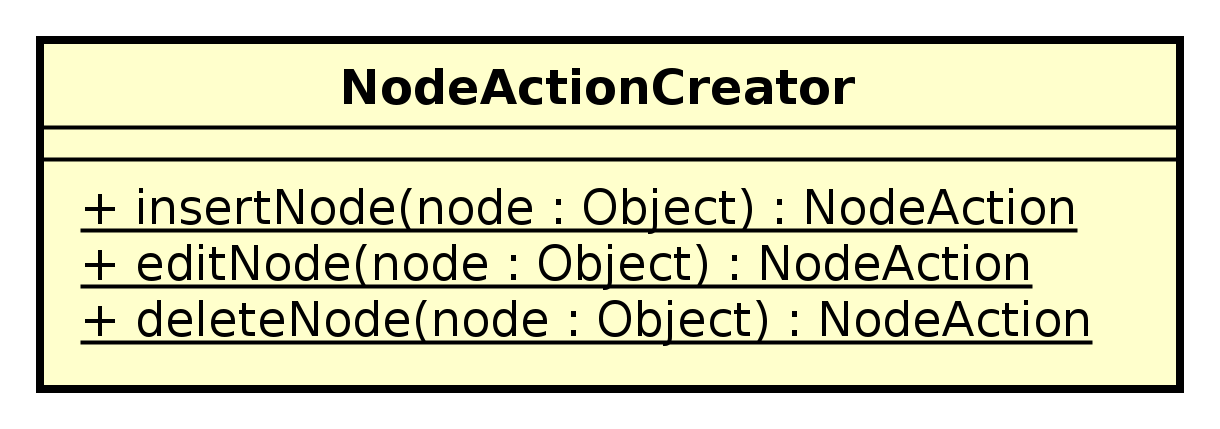
\includegraphics[width=0.3\textwidth]{./img/NodeActionCreator.png}
		\caption{Diagramma classe NodeActionCreator}
	\end{figure}
	\item \textbf{descrizione:} rappresenta la factory di azioni relative ai nodi;
	\item \textbf{utilizzo:} i suoi metodi sono chiamati dalla View e dal CallManager per la creazione di azioni relative ai nodi;
	\item \textbf{metodi:}
	\begin{itemize}
		\item +deleteNode(node) : NodeAction\newline
		il metodo crea l'azione relativa all'eliminazione di un nodo
		\begin{itemize}
			\item node : Object\\
			oggetto contenente i parametri di un nodo che dovrà essere eliminato.
		\end{itemize}
		\item +editNode(node) : NodeAction\newline
		il metodo crea l'azione relativa alla modifica di un nodo
		\begin{itemize}
			\item node : Object\\
			oggetto contenente i parametri di un nodo che dovrà essere modificato nello store.
		\end{itemize}
		\item +insertNode(node) : NodeAction\newline
		il metodo crea l'azione relativa all'inserimento di un nuovo nodo
		\begin{itemize}
			\item node : Object\\
			oggetto contenente i parametri di un nodo che dovrà essere inserito nello store.
		\end{itemize}
	\end{itemize}
\end{itemize}
\paragraph{OptionActionCreator}
\begin{itemize}
	\begin{figure}[H]
		\centering
		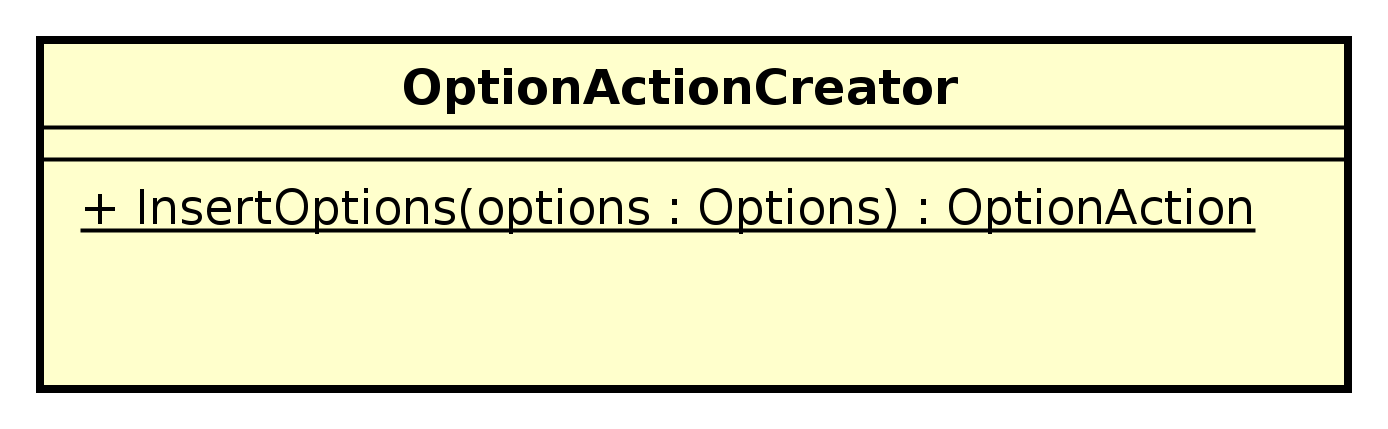
\includegraphics[width=0.3\textwidth]{./img/OptionActionCreator.png}
		\caption{Diagramma classe OptionActionCreator}
	\end{figure}
	\item \textbf{descrizione:} rappresenta la factory di azioni relative agli asset;
	\item \textbf{utilizzo:} i suoi metodi sono chiamati dalla View e dal CallManager per la creazione di azioni relative agli asset;
	\item \textbf{metodi:}
	\begin{itemize}
		\item +insertOptions() : OptionAction\newline
		il metodo crea l'azione relativa all'inserimento dell'oggetto options dello store
	\end{itemize}
	\item \textbf{relazioni con altre classi:} 
	\begin{itemize}
		\item OUT OptionAction.
	\end{itemize}
\end{itemize}
\newpage
\subsection{DeGeOP::ViewPkg}
\label{pkg::ViewPkg}
\begin{figure}[H]
	\centering
	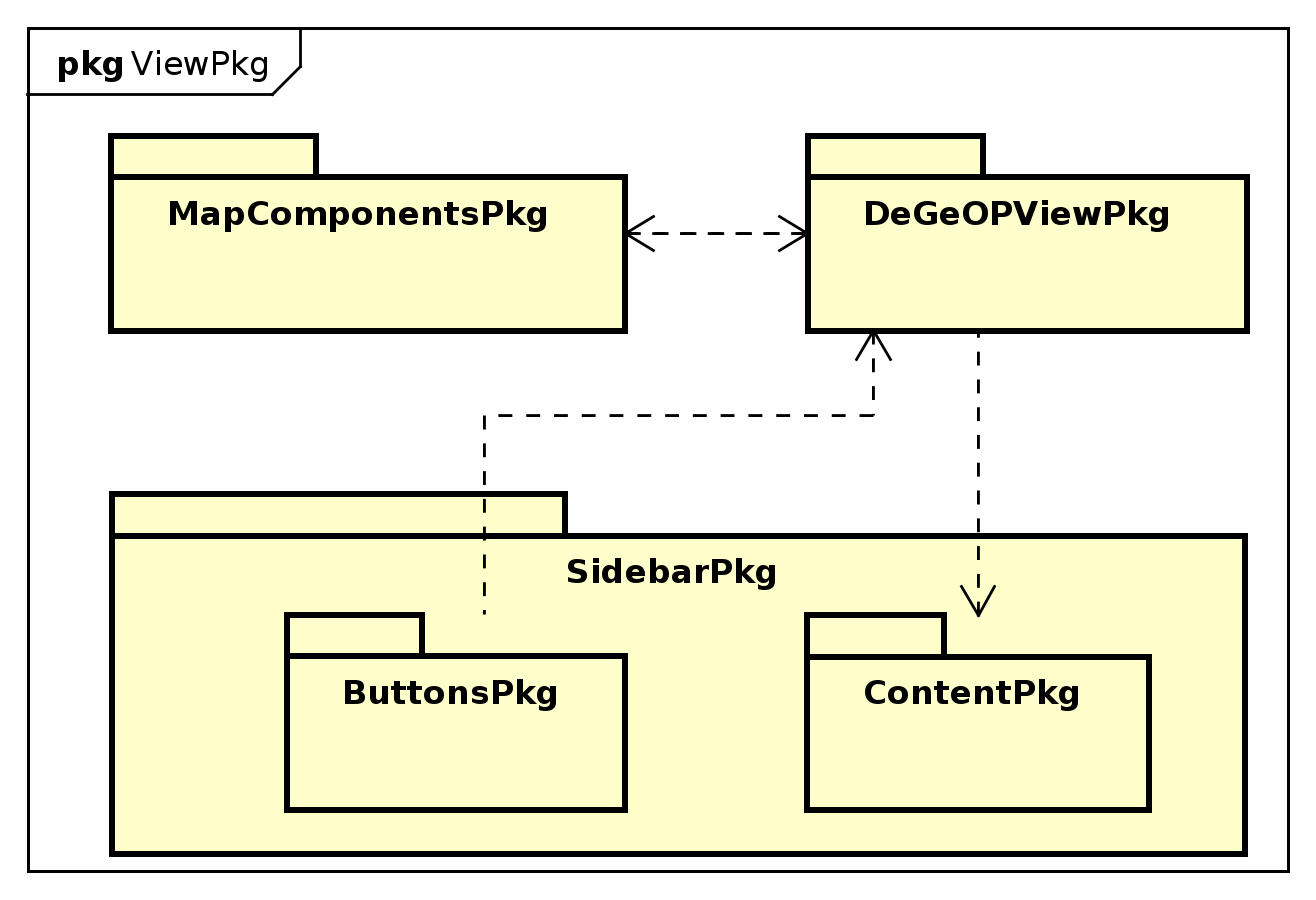
\includegraphics[width=\textwidth]{img/PkgDiagram/ViewPkg.png}
	\caption{Schema componente DeGeOP::ViewPkg}
\end{figure}
\subsubsection{Informazioni sul package}
\begin{itemize}
	\item \textbf{descrizione:} racchiude le componenti per la visualizzazione dell'interfaccia utente;
	\item \textbf{padre:} \hyperref[pkg::DeGeOP]{DeGeOP};
	\item \textbf{package contenuti:}
	\begin{itemize}
		\item ViewPkg::\hyperref[pkg::DeGeOPViewPkg]{DeGeOPViewPkg};
		\item ViewPkg::\hyperref[pkg::MapComponentsPkg]{MapComponentsPkg};
		\item ViewPkg::\hyperref[pkg::SidebarPkg]{SidebarPkg}.
	\end{itemize}
	\item \textbf{interazioni con altri package:} 
	\begin{itemize}
		\item OUT ActionPkg: dispatch di azioni;
		\item OUT Alexa voice service: gestore vocale;
		\item OUT Hammer: gestione gesture ;
		\item OUT Openlayers: gestione mappa;
		\item OUT React: utilizzo componenti react;
		\item OUT ReactToolbox: utilizzo componenti material design;
		\item OUT Redux: utilizzo metodo dispatch;
		\item OUT StorePkg: subscribe sullo store.
	\end{itemize}
\end{itemize}
\newpage
\subsection{DeGeOP::ViewPkg::DeGeOPViewPkg}
\label{pkg::DeGeOPViewPkg}
\begin{figure}[H]
	\centering
	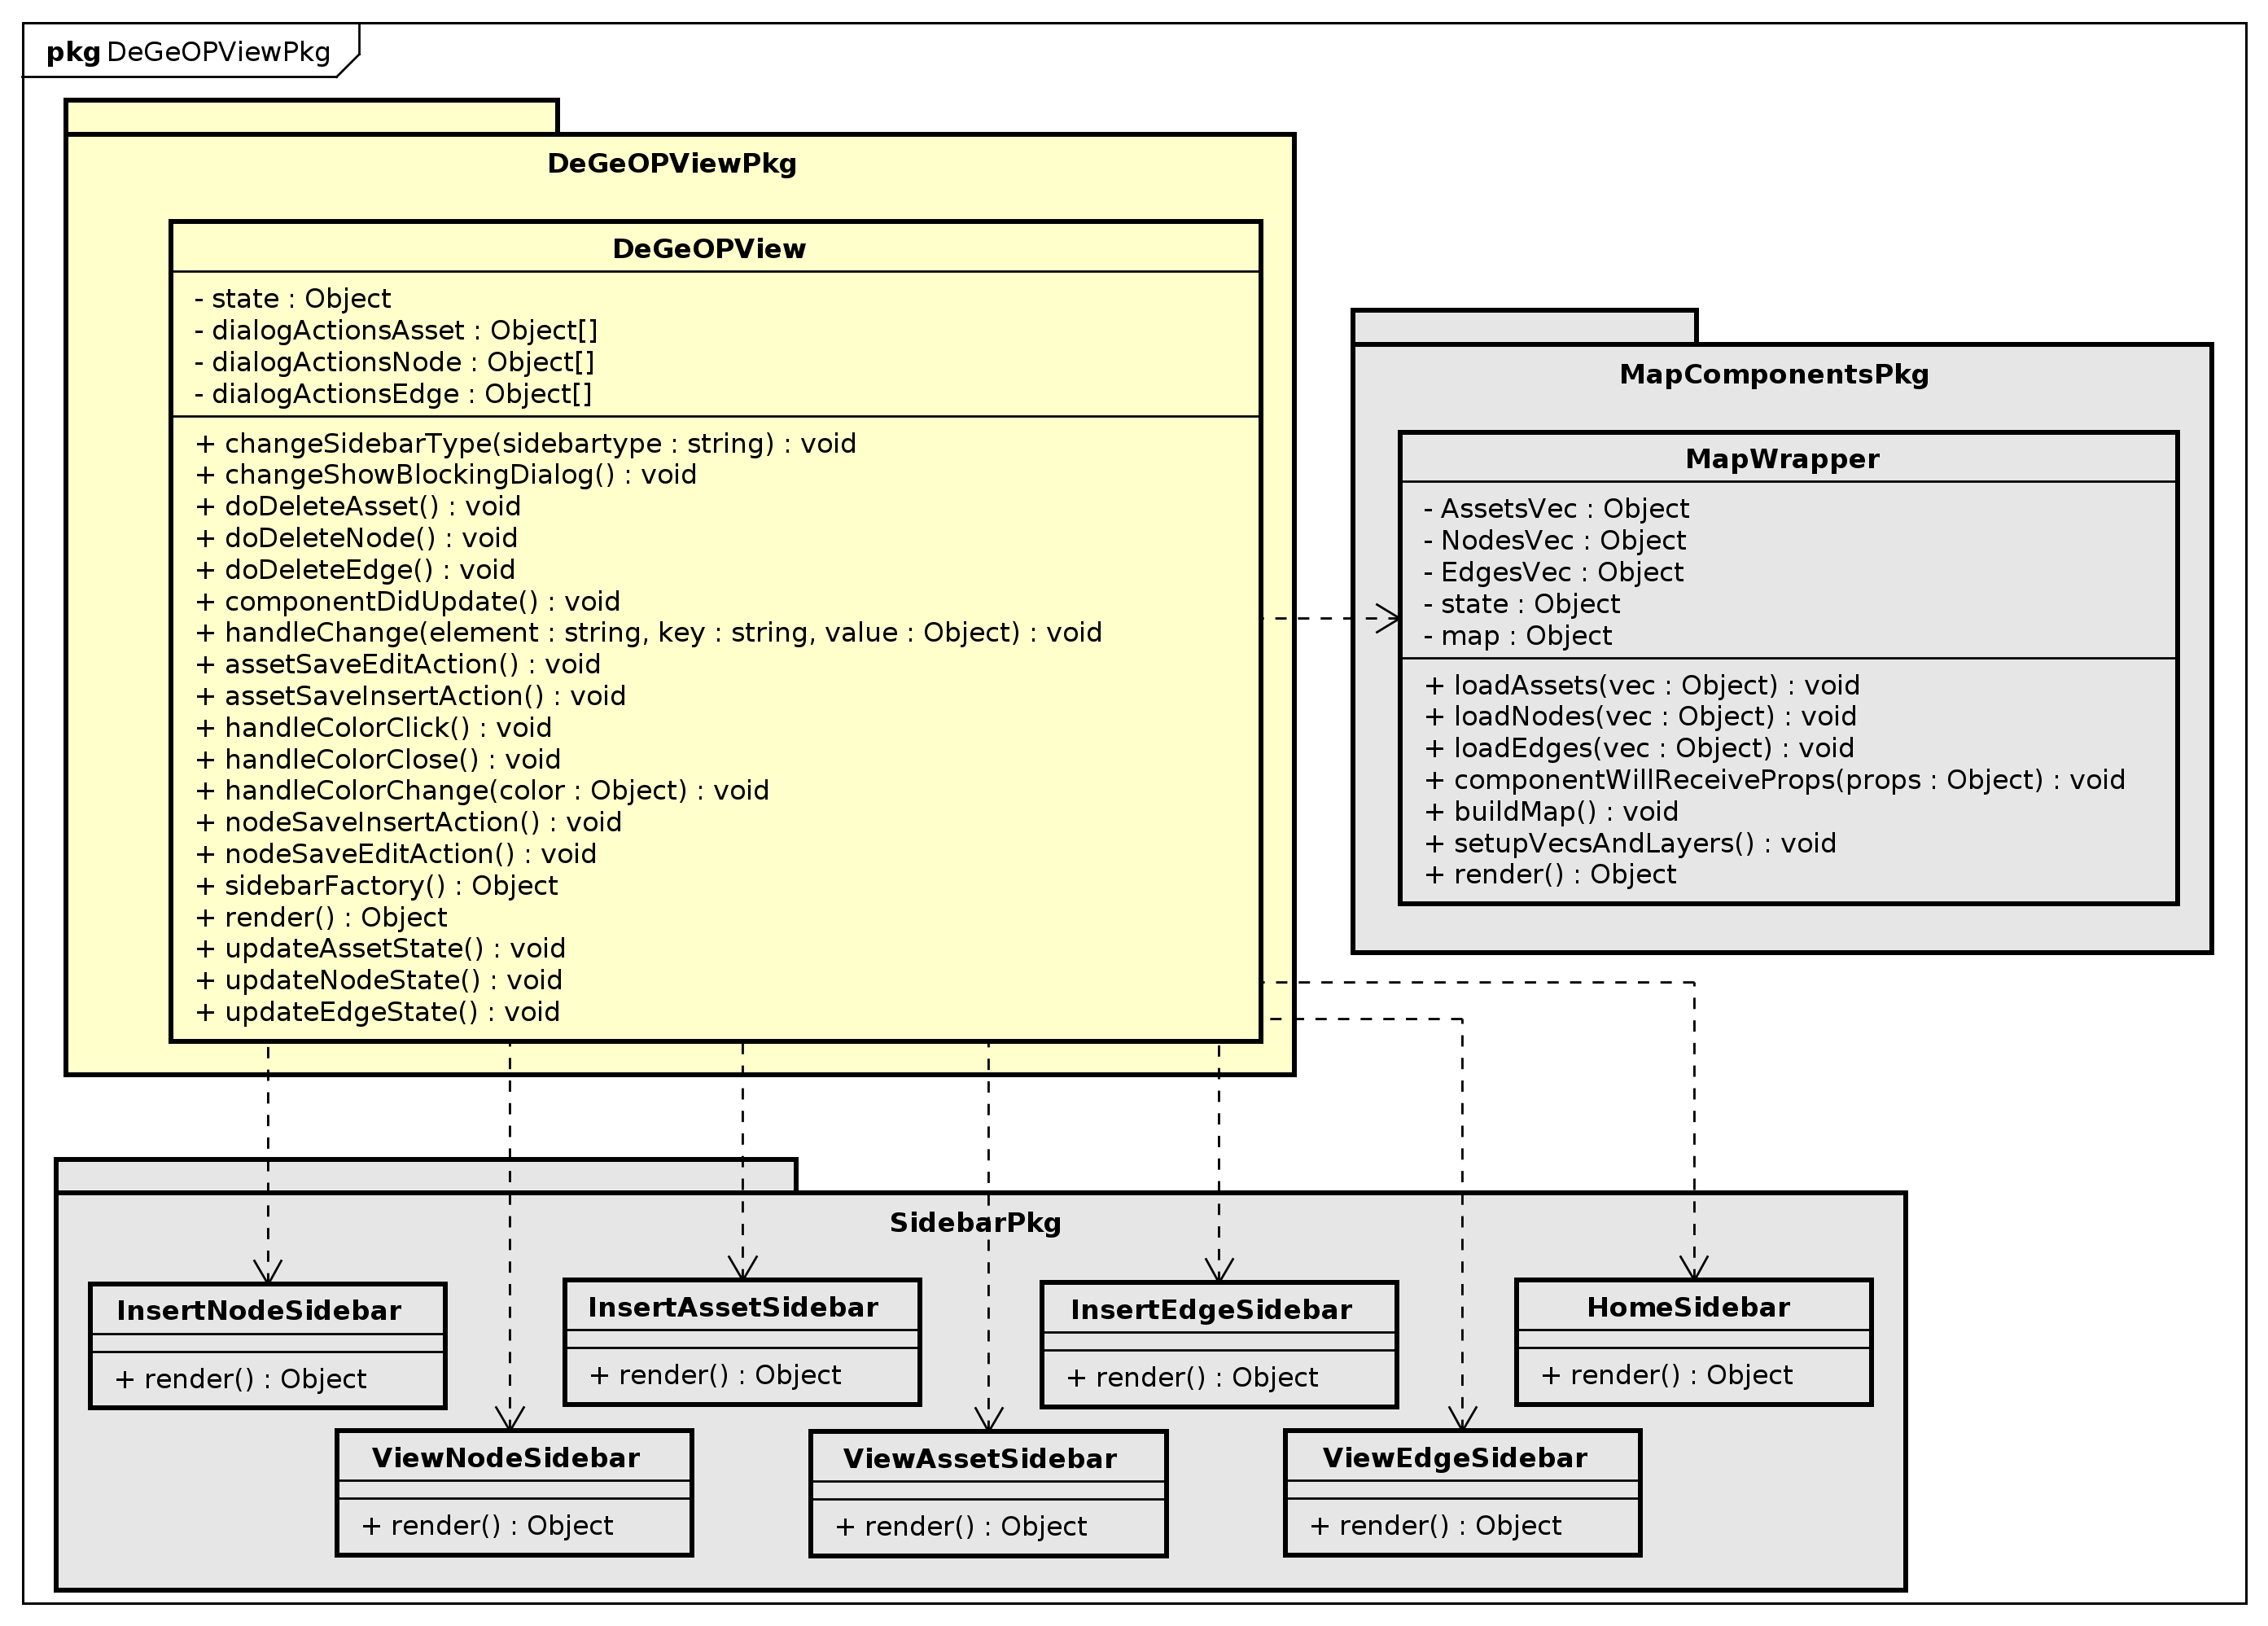
\includegraphics[width=\textwidth]{img/PkgDiagram/DeGeOPViewPkg.png}
	\caption{Schema componente DeGeOP::ViewPkg::DeGeOPViewPkg}
\end{figure}
\subsubsection{Informazioni sul package}
\begin{itemize}
	\item \textbf{descrizione:} racchiude la componente principale della view;
	\item \textbf{padre:} \hyperref[pkg::ViewPkg]{ViewPkg};
	\item \textbf{interazioni con altri package:} 
	\begin{itemize}
		\item IN MapComponentsPkg: utilizzo di componenti grafiche;
		\item OUT MapComponentsPkg: utilizzo di componenti grafiche;
		\item OUT SidebarPkg: utilizzo della sidebar.
	\end{itemize}
	\item \textbf{classi contenute:}
	\begin{itemize}
		\item DeGeOPView.
	\end{itemize}
\end{itemize}
\subsubsection{Classi}
\paragraph{DeGeOPView}
\begin{itemize}
	\begin{figure}[H]
		\centering
		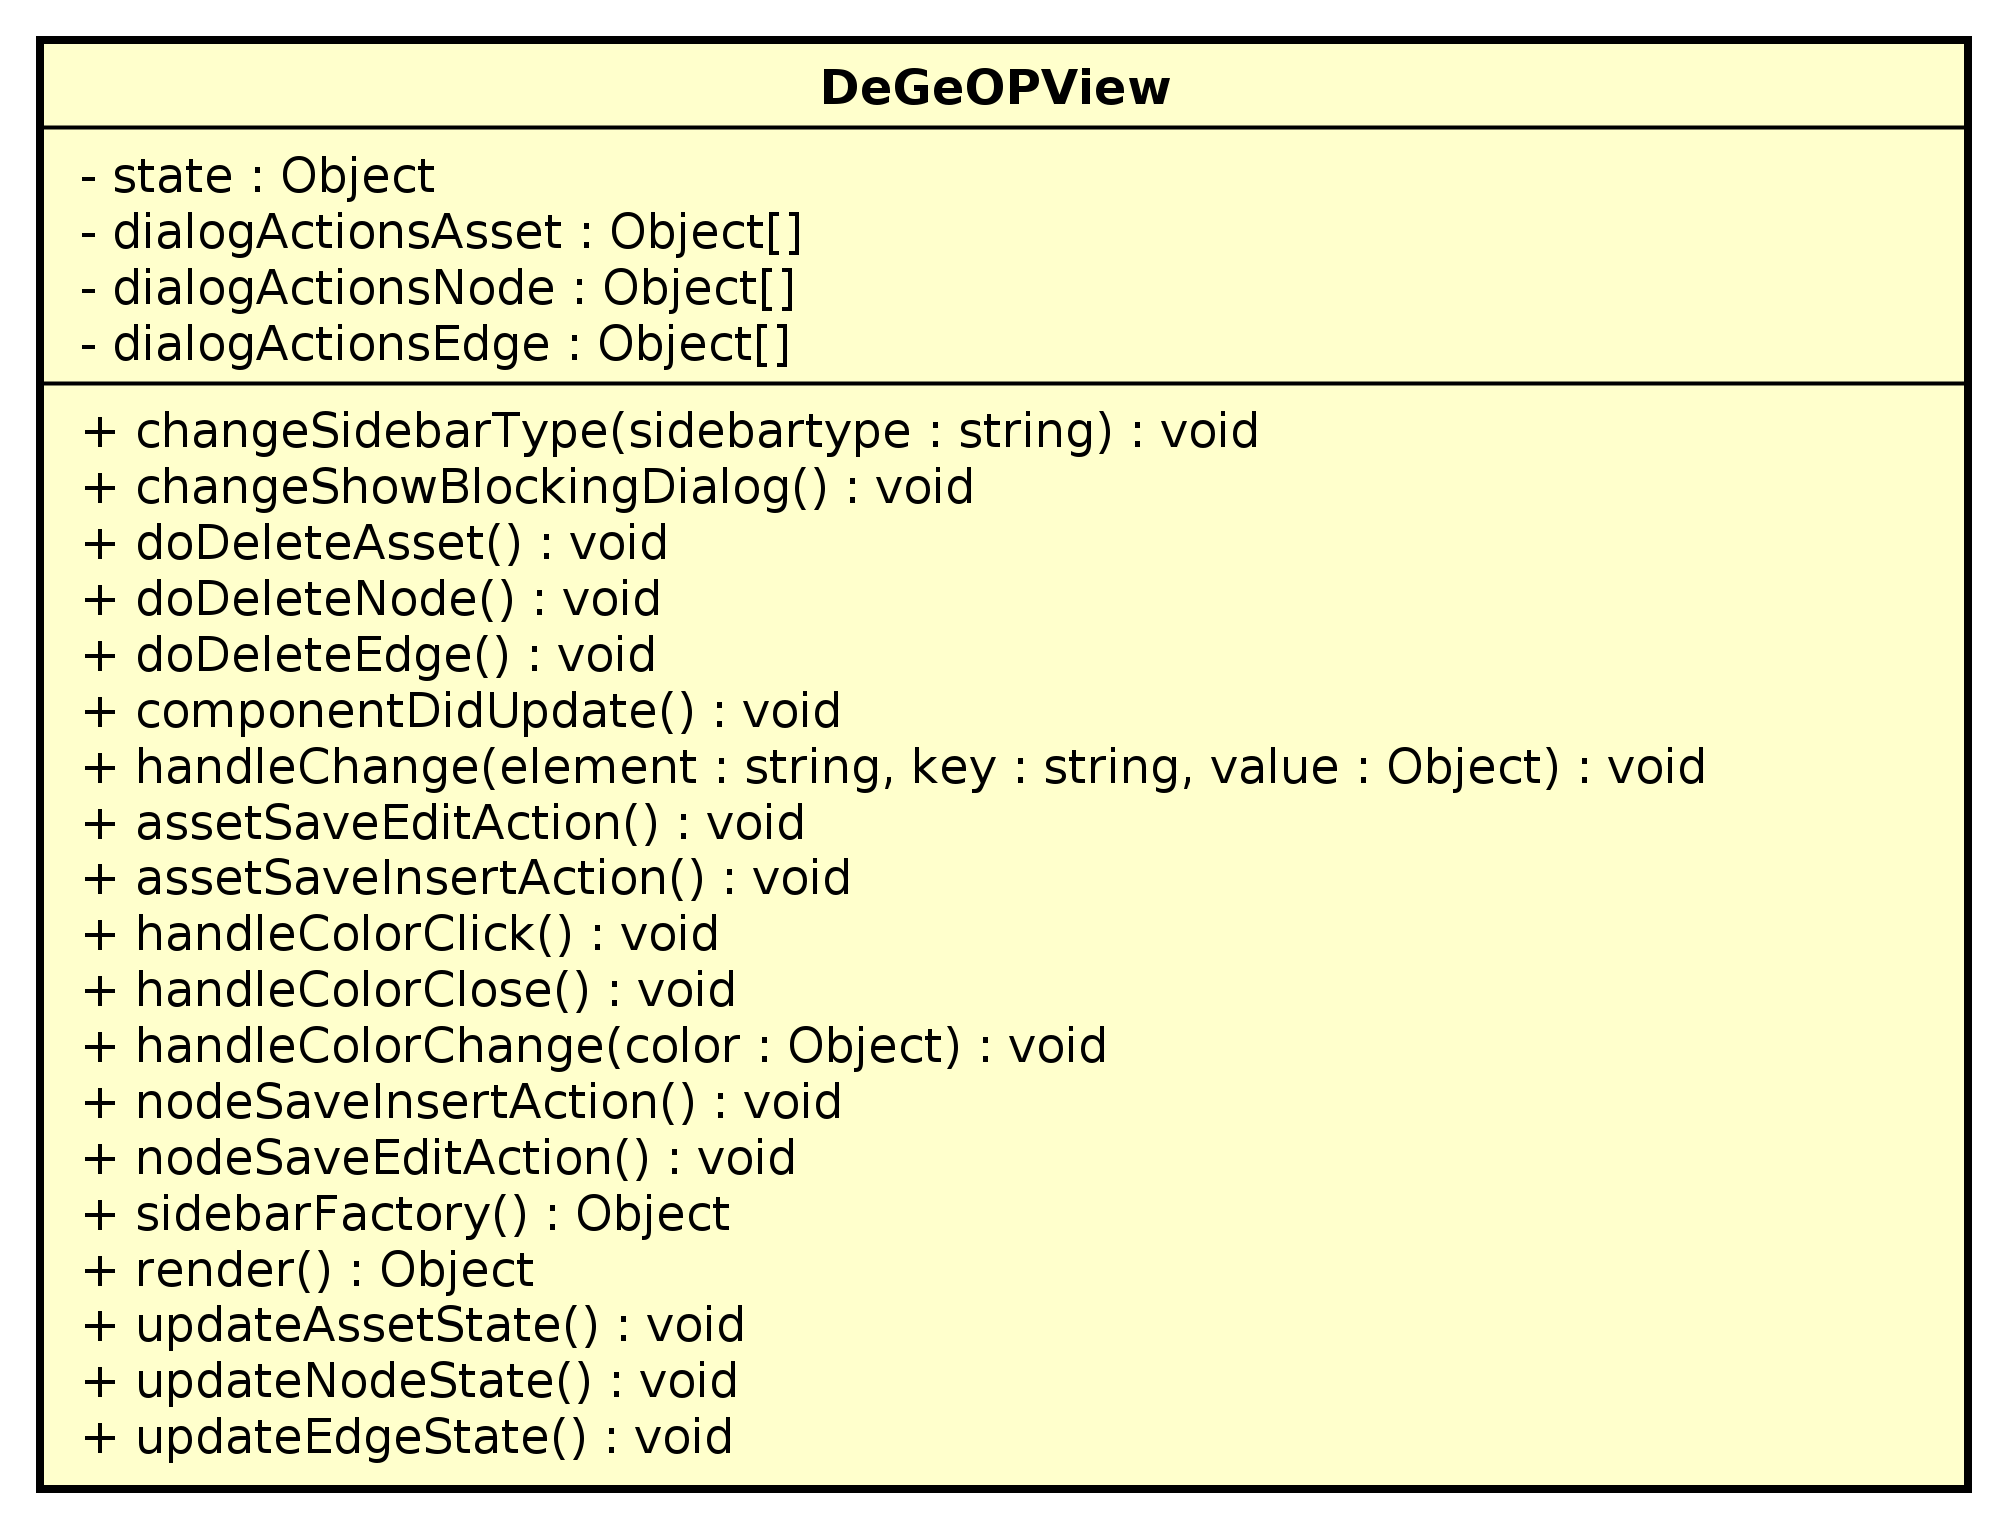
\includegraphics[width=0.3\textwidth]{./img/DeGeOPView.png}
		\caption{Diagramma classe DeGeOPView}
	\end{figure}
	\item \textbf{descrizione:} rappresenta l'oggetto grafico radice, che comprende l'intera View del prodotto;
	\item \textbf{utilizzo:} i suoi metodi setter sono richiamati da ConcreteDeGeOPViewBuilder per impostare i suoi campi dati. La classe effettua il subscribe sullo Store per ricevere gli aggiornamenti ;
	\item \textbf{attributi:}
	\begin{itemize}
		\item -dialogActionsAsset : Object[]\begin{itemize}
			\item contiene le funzioni richiamate durante la visualizzazione della schermata modale relativa agli asset.\end{itemize}
		\item -dialogActionsEdge : Object[]\begin{itemize}
			\item contiene le funzioni richiamate durante la visualizzazione della schermata modale relativa ai nodi.\end{itemize}
		\item -dialogActionsNode : Object[]\begin{itemize}
			\item contiene le funzioni richiamate durante la visualizzazione della schermata modale relativa ai nodi.\end{itemize}
		\item -state : Object\begin{itemize}
			\item rappresenta lo stato di DeGeOPView, ovvero i dati temporanei che l'utente inserisce prima che vengano inseriti nello store.\end{itemize}
	\end{itemize}
	\item \textbf{metodi:}
	\begin{itemize}
		\item +assetSaveEditAction() : void\newline
		il metodo emette l'azione relativa alla modifica di un asset
		\item +assetSaveInsertAction() : void\newline
		il metodo emette l'azione relativa all'inserimento di un asset
		\item +changeShowBlockingDialog() : void\newline
		il metodo gestisce il cambiamento del booleano nello state di DeGeOPView che gestisce la visualizzazione della finestra modale
		\item +changeSidebarType() : void\newline
		il metodo gestisce il cambiamento della stringa dello state di DeGeOPView che gestisce il tipo di sidebar visualizzata al momento
		\item +componentDidUpdate() : void\newline
		il metodo viene richiamato quando lo state di DeGeOPView cambia; al suo interno vengono gestite le validazioni dei campi compilati dall'utente
		\item +doDeleteAsset() : void\newline
		il metodo emette l'azione di eliminazione dell'asset attualmente selezionato e ne fa il dispatch verso lo store
		\item +doDeleteEdge() : void\newline
		il metodo emette l'azione di eliminazione del nodo attualmente selezionato e ne fa il dispatch verso lo store
		\item +doDeleteNode() : void\newline
		il metodo emette l'azione di eliminazione del nodo attualmente selezionato e ne fa il dispatch verso lo store
		\item +handleChange(element, key, value) : void\newline
		il metodo gestisce il cambiamento di stato di DeGeOPView relativamente ai campi dati compilati dall'utente
		\begin{itemize}
			\item element : string\\
			indica il campo dati dello stato di DeGeOPView da cambiare. Può assumere i valori:
			asset, node, edge, common.
			\item key : string\\
			indica il campo dati dell'oggetto descritto da element che dovrà essere modificato.
			\item value : Object\\
			indica il valore da inserire nell'oggetto descritto da element, nel campo dati descritto da key.
		\end{itemize}
		\item +handleColorChange(color) : void\newline
		il metodo gestisce il cambiamento nello state di DeGeOPView relativo al colore selezionato dalla palette colori
		\begin{itemize}
			\item color : Object\\
			rappresenta il nuovo colore selezionato dalla palette colori.
		\end{itemize}
		\item +handleColorClick() : void\newline
		il metodo gestisce l'apertura e la chiusura della palette colori
		\item +handleColorClose() : void\newline
		il metodo gestisce la chiusura della palette colori
		\item +nodeSaveEditAction() : void\newline
		il metodo gestisce l'emissione dell'azione relativa alla modifica di un nodo
		\item +nodeSaveInsertAction() : void\newline
		il metodo gestisce l'emissione dell'azione relativa all'inserimento di un nodo
		\item +render() : Object\newline
		il metodo gestisce il render di DeGeOPView, composta da una sidebar e da un MapWrapper
		\item +sidebarFactory() : Object\newline
		il metodo gestisce la creazione di una sidebar da renderizzare in base alla stringa attualmente specificata nello state di DeGeOPView
		\item +updateAssetState() : void\newline
		il metodo imposta lo stato dell'asset in DeGeOPView con i dati dell'asset selezionato sulla mappa
		\item +updateEdgeState() : void\newline
		il metodo imposta lo stato dell'arco in DeGeOPView con i dati dell'arco selezionato sulla mappa
		\item +updateNodeState() : void\newline
		il metodo imposta lo stato del nodo in DeGeOPView con i dati del nodo selezionato sulla mappa
	\end{itemize}
\end{itemize}
\newpage
\subsection{DeGeOP::ViewPkg::MapComponentsPkg}
\label{pkg::MapComponentsPkg}
\begin{figure}[H]
	\centering
	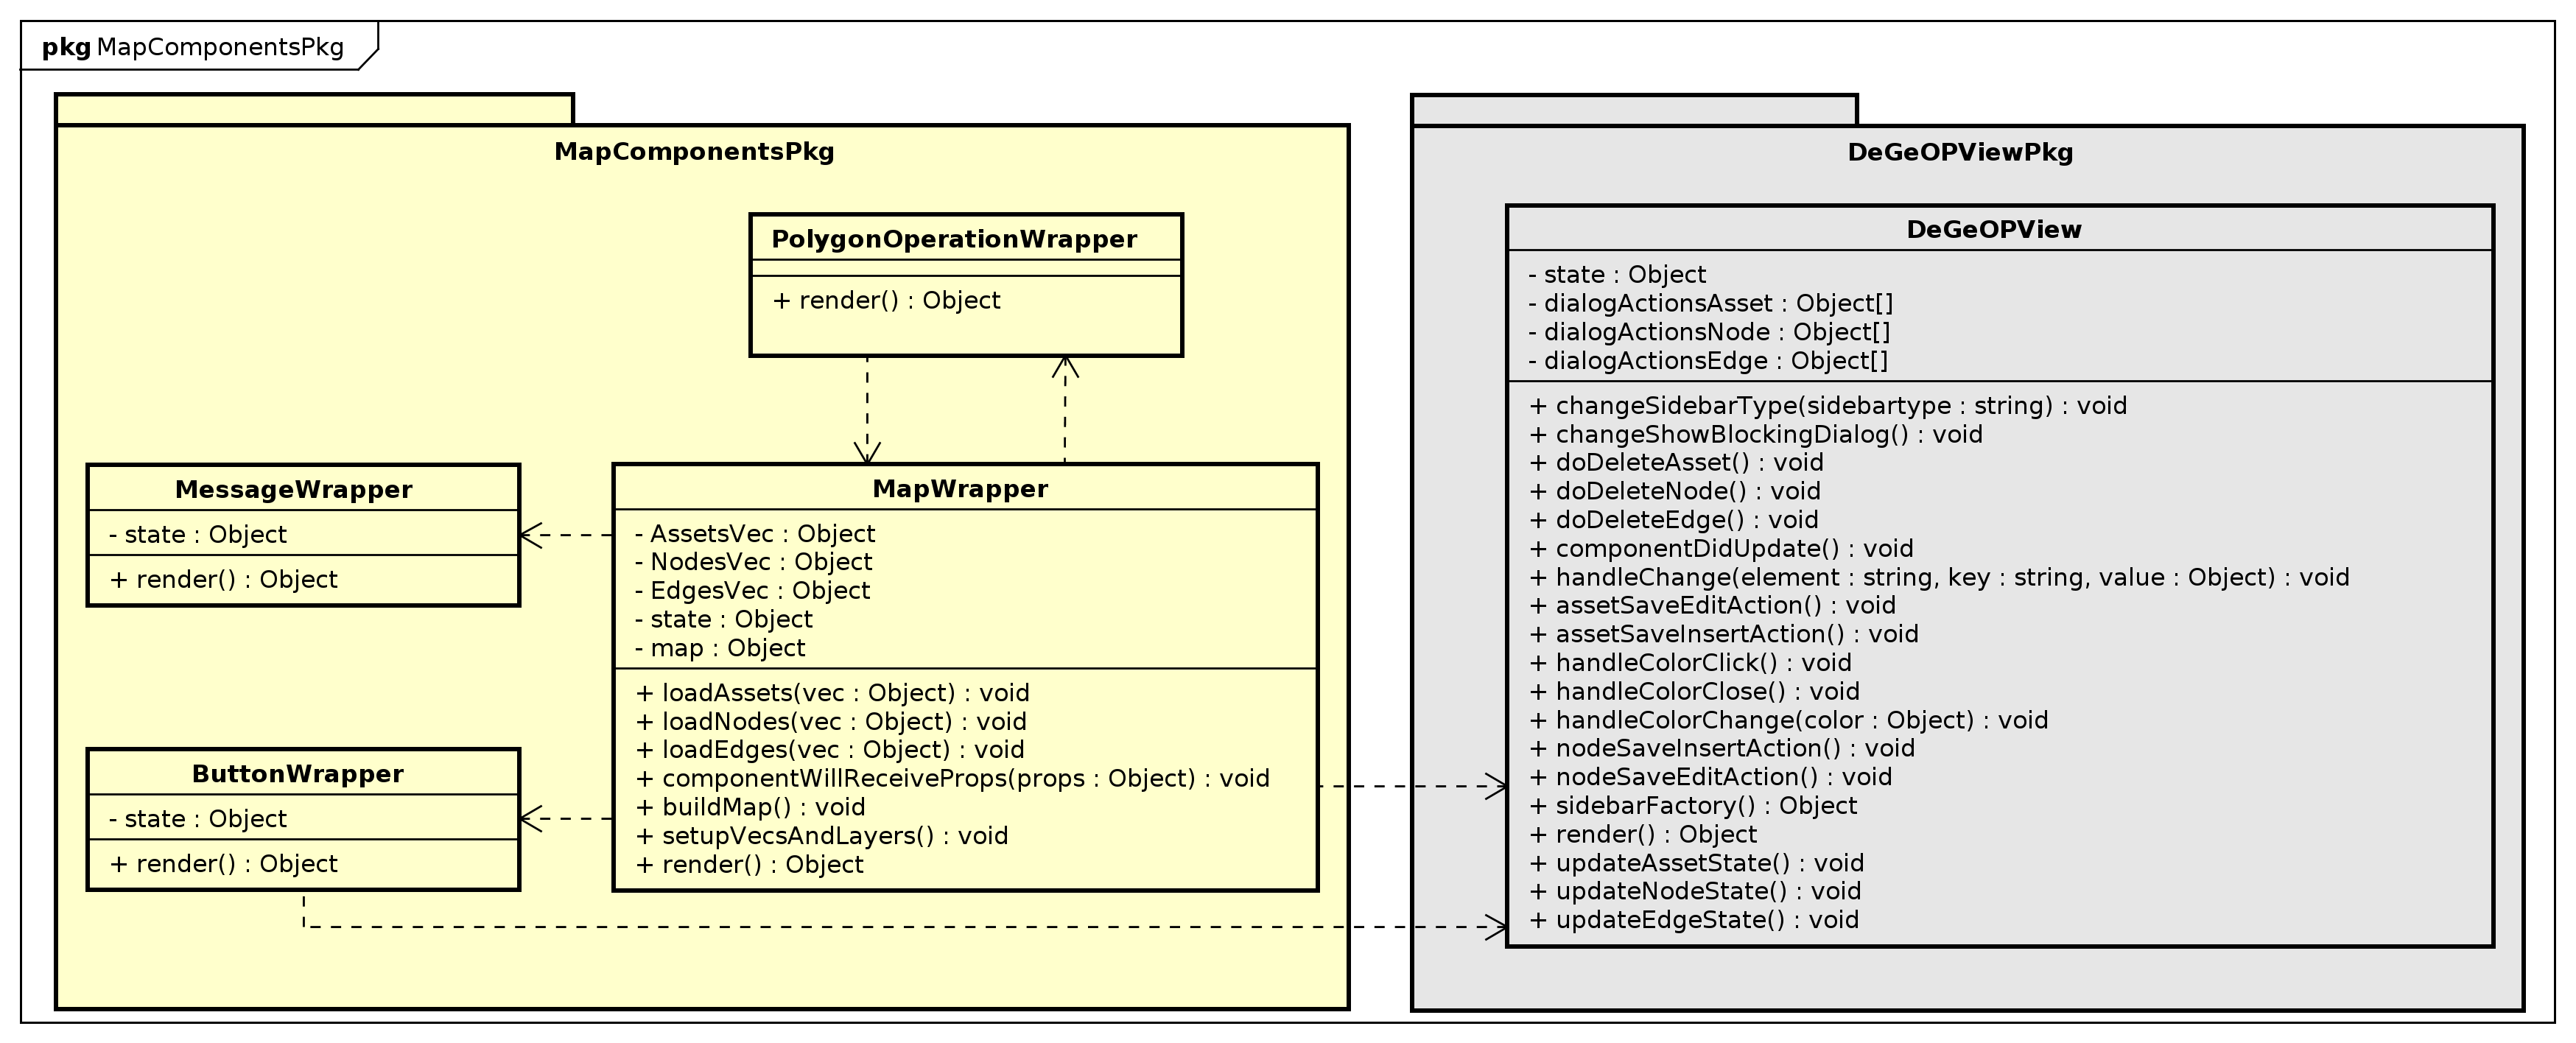
\includegraphics[width=\textwidth]{img/PkgDiagram/MapComponentsPkg.png}
	\caption{Schema componente DeGeOP::ViewPkg::MapComponentsPkg}
\end{figure}
\subsubsection{Informazioni sul package}
\begin{itemize}
	\item \textbf{descrizione:} racchiude le componenti relative alla mappa e ai pulsanti sopra di essa;
	\item \textbf{padre:} \hyperref[pkg::ViewPkg]{ViewPkg};
	\item \textbf{interazioni con altri package:} 
	\begin{itemize}
		\item IN DeGeOPViewPkg: utilizzo di componenti grafiche;
		\item OUT DeGeOPViewPkg: utilizzo di componenti grafiche;
		\item OUT Openlayers: gestione mappa.
	\end{itemize}
	\item \textbf{classi contenute:}
	\begin{itemize}
		\item ButtonWrapper;
		\item MapWrapper;
		\item MessageWrapper;
		\item PolygonOperationWrapper.
	\end{itemize}
\end{itemize}
\subsubsection{Classi}
\paragraph{ButtonWrapper}
\begin{itemize}
	\begin{figure}[H]
		\centering
		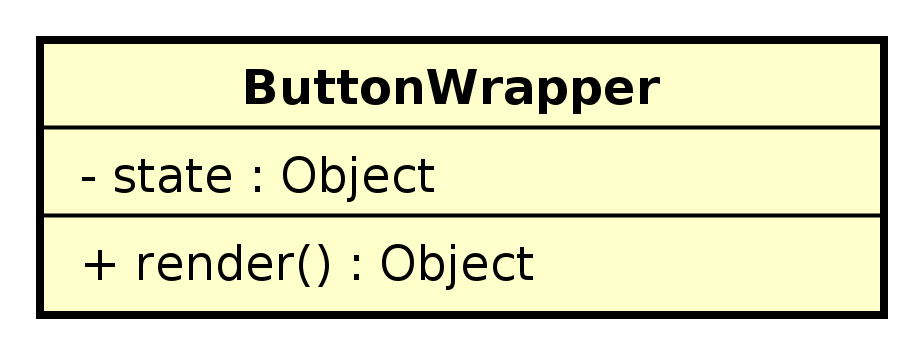
\includegraphics[width=0.3\textwidth]{./img/ButtonWrapper.png}
		\caption{Diagramma classe ButtonWrapper}
	\end{figure}
	\item \textbf{descrizione:} rappresenta una classe wrapper per visualizzare una serie di bottoni con cui è possibile eseguire varie operazioni;
	\item \textbf{utilizzo:} viene utilizzato per mostrare sulla mappa una serie di bottoni;
	\item \textbf{attributi:}
	\begin{itemize}
		\item -state : Object\begin{itemize}
			\item rappresenta lo stato del ButtonWrapper.\end{itemize}
	\end{itemize}
	\item \textbf{relazioni con altre classi:} 
	\begin{itemize}
		\item IN MapWrapper.
	\end{itemize}
\end{itemize}
\paragraph{MapWrapper}
\begin{itemize}
	\begin{figure}[H]
		\centering
		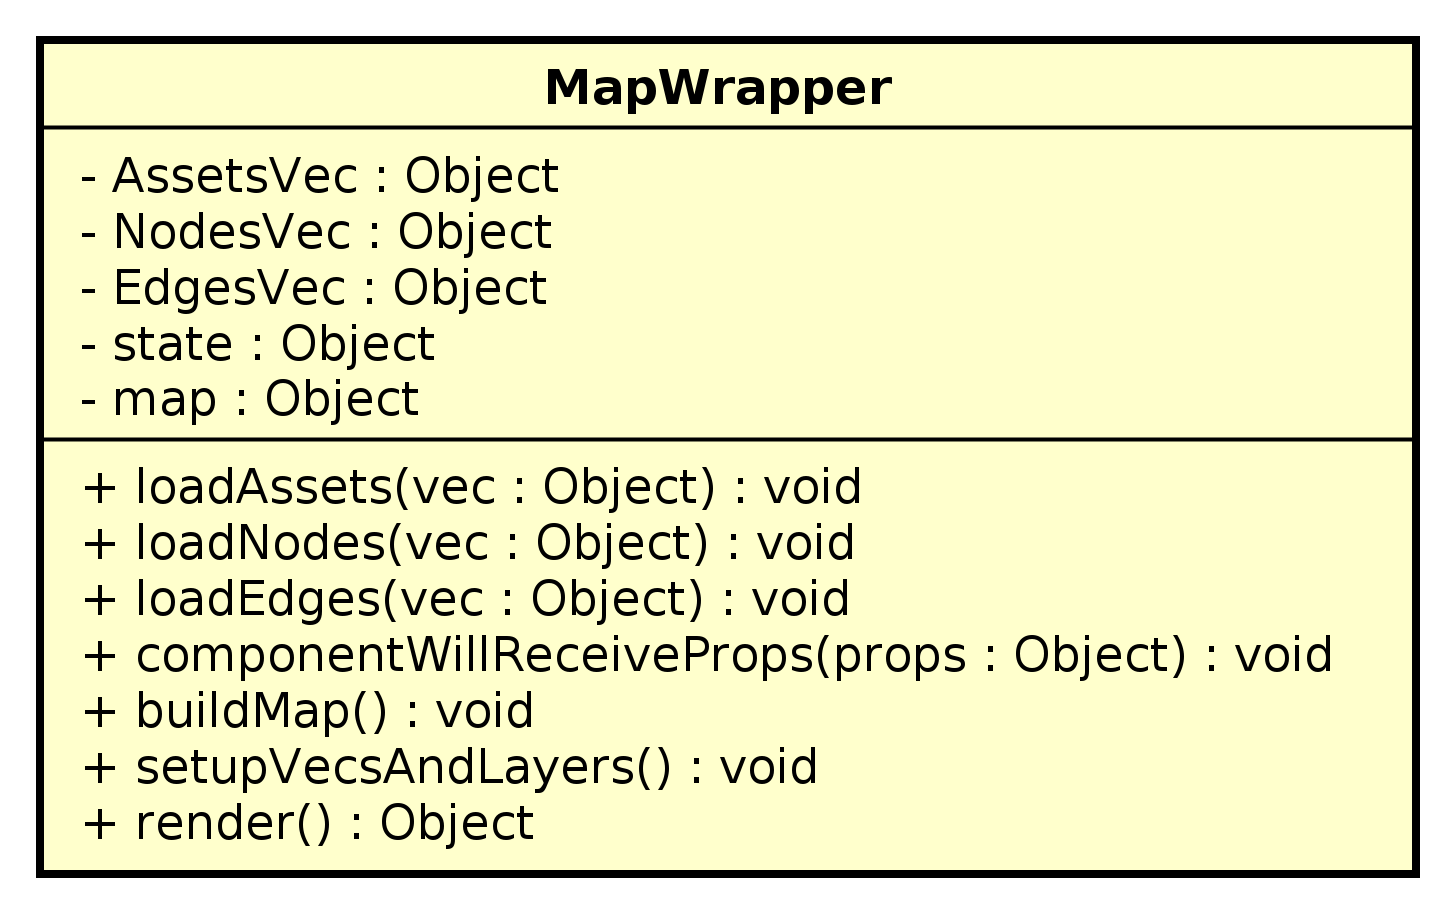
\includegraphics[width=0.3\textwidth]{./img/MapWrapper.png}
		\caption{Diagramma classe MapWrapper}
	\end{figure}
	\item \textbf{descrizione:} rappresenta una classe wrapper per visualizzare la mappa;
	\item \textbf{utilizzo:} viene utilizzata per visualizzare una mappa e permettere all'utente di interagire con essa;
	\item \textbf{attributi:}
	\begin{itemize}
		\item -assetsVec : Object\begin{itemize}
			\item contiene gli oggetti geometrici relativi agli asset da disegnare sulla mappa.\end{itemize}
		\item -edgesVec : Object\begin{itemize}
			\item contiene gli oggetti geometrici relativi agli asset da disegnare sulla mappa.\end{itemize}
		\item -map : Object\begin{itemize}
			\item oggetto che contiene lo stato della mappa.\end{itemize}
		\item -nodesVec : Object\begin{itemize}
			\item contiene gli oggetti geometrici relativi ai nodi da disegnare sulla mappa.\end{itemize}
		\item -state : Object\begin{itemize}
			\item contiene lo stato della classe MapWrapper.\end{itemize}
	\end{itemize}
	\item \textbf{metodi:}
	\begin{itemize}
		\item +buildMap() : void\newline
		il metodo costruisce la mappa
		\item +componentWillReceiveProps(props) : void\newline
		il metodo viene richiamato quando la componente MapWrapper sta per ricevere nuovi props
		\begin{itemize}
			\item props : Object\\
			props da ricevere.
		\end{itemize}
		\item +loadAssets(vec) : void\newline
		il metodo carica il vettore degli asset
		\begin{itemize}
			\item vec : Object\\
			vettore degli asset da caricare.
		\end{itemize}
		\item +loadEdges(vec) : void\newline
		il metodo carica il vettore degli archi
		\begin{itemize}
			\item vec : Object\\
			vettore degli archi da caricare.
		\end{itemize}
		\item +loadNodes(vec) : void\newline
		il metodo carica il vettore dei nodi
		\begin{itemize}
			\item vec : Object\\
			vettore dei nodi da caricare.
		\end{itemize}
		\item +render() : Object\newline
		renderizza il MapWrapper
		\item +setupVecsAndLayers() : void\newline
		il metodo prepara i vettori e i layers per la mappa
	\end{itemize}
	\item \textbf{relazioni con altre classi:} 
	\begin{itemize}
		\item IN PolygonOperationWrapper;
		\item OUT ButtonWrapper;
		\item OUT MessageWrapper;
		\item OUT PolygonOperationWrapper.
	\end{itemize}
\end{itemize}
\paragraph{MessageWrapper}
\begin{itemize}
	\begin{figure}[H]
		\centering
		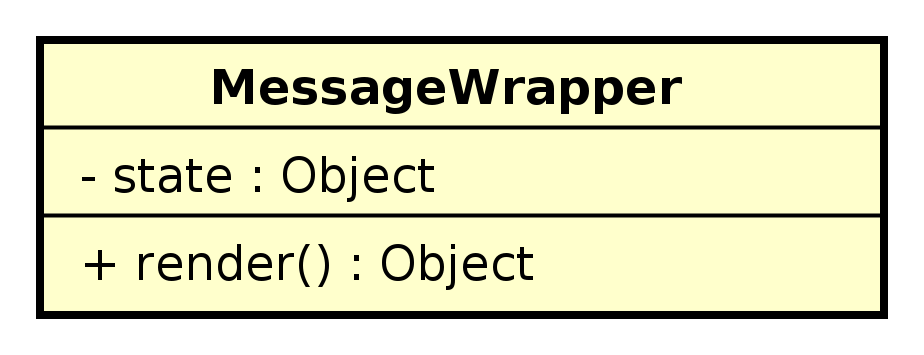
\includegraphics[width=0.3\textwidth]{./img/MessageWrapper.png}
		\caption{Diagramma classe MessageWrapper}
	\end{figure}
	\item \textbf{descrizione:} rappresenta una classe wrapper per visualizzare un messaggio;
	\item \textbf{utilizzo:} viene utilizzato per mostrare messaggi di errore o di successo sulla mappa;
	\item \textbf{attributi:}
	\begin{itemize}
		\item -state : Object\begin{itemize}
			\item rappresenta lo stato del MessageWrapper.\end{itemize}
	\end{itemize}
	\item \textbf{metodi:}
	\begin{itemize}
		\item +render() : Object\newline
		renderizza il MessageWrapper
	\end{itemize}
	\item \textbf{relazioni con altre classi:} 
	\begin{itemize}
		\item IN MapWrapper.
	\end{itemize}
\end{itemize}
\paragraph{PolygonOperationWrapper}
\begin{itemize}
	\begin{figure}[H]
		\centering
		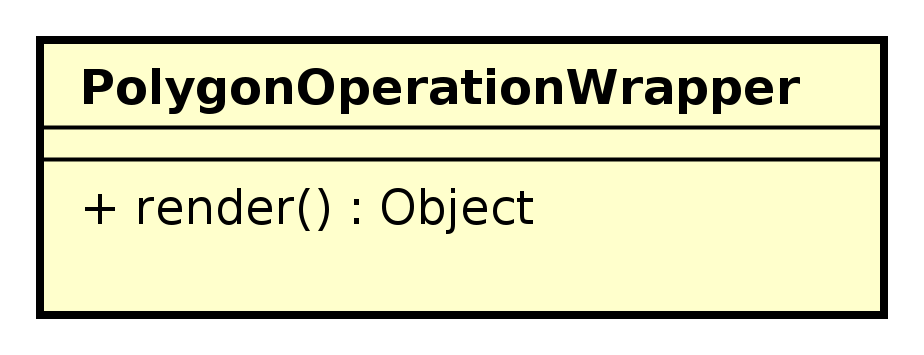
\includegraphics[width=0.3\textwidth]{./img/PolygonOperationWrapper.png}
		\caption{Diagramma classe PolygonOperationWrapper}
	\end{figure}
	\item \textbf{descrizione:} rappresenta una classe wrapper per visualizzare un bottone con cui è possibile effettuare operazioni sul perimetro di un poligono sulla mappa;
	\item \textbf{utilizzo:} invocando i suoi metodi è possibile iniziare a disegnare il poligono su mappa oppure cancellare l'ultimo segmento disegnato;
	\item \textbf{metodi:}
	\begin{itemize}
		\item +render() : Object\newline
		renderizza il PolygonOperationWrapper
	\end{itemize}
	\item \textbf{relazioni con altre classi:} 
	\begin{itemize}
		\item IN MapWrapper;
		\item OUT MapWrapper.
	\end{itemize}
\end{itemize}
\newpage
\subsection{DeGeOP::ViewPkg::SidebarPkg}
\label{pkg::SidebarPkg}
\begin{figure}[H]
	\centering
	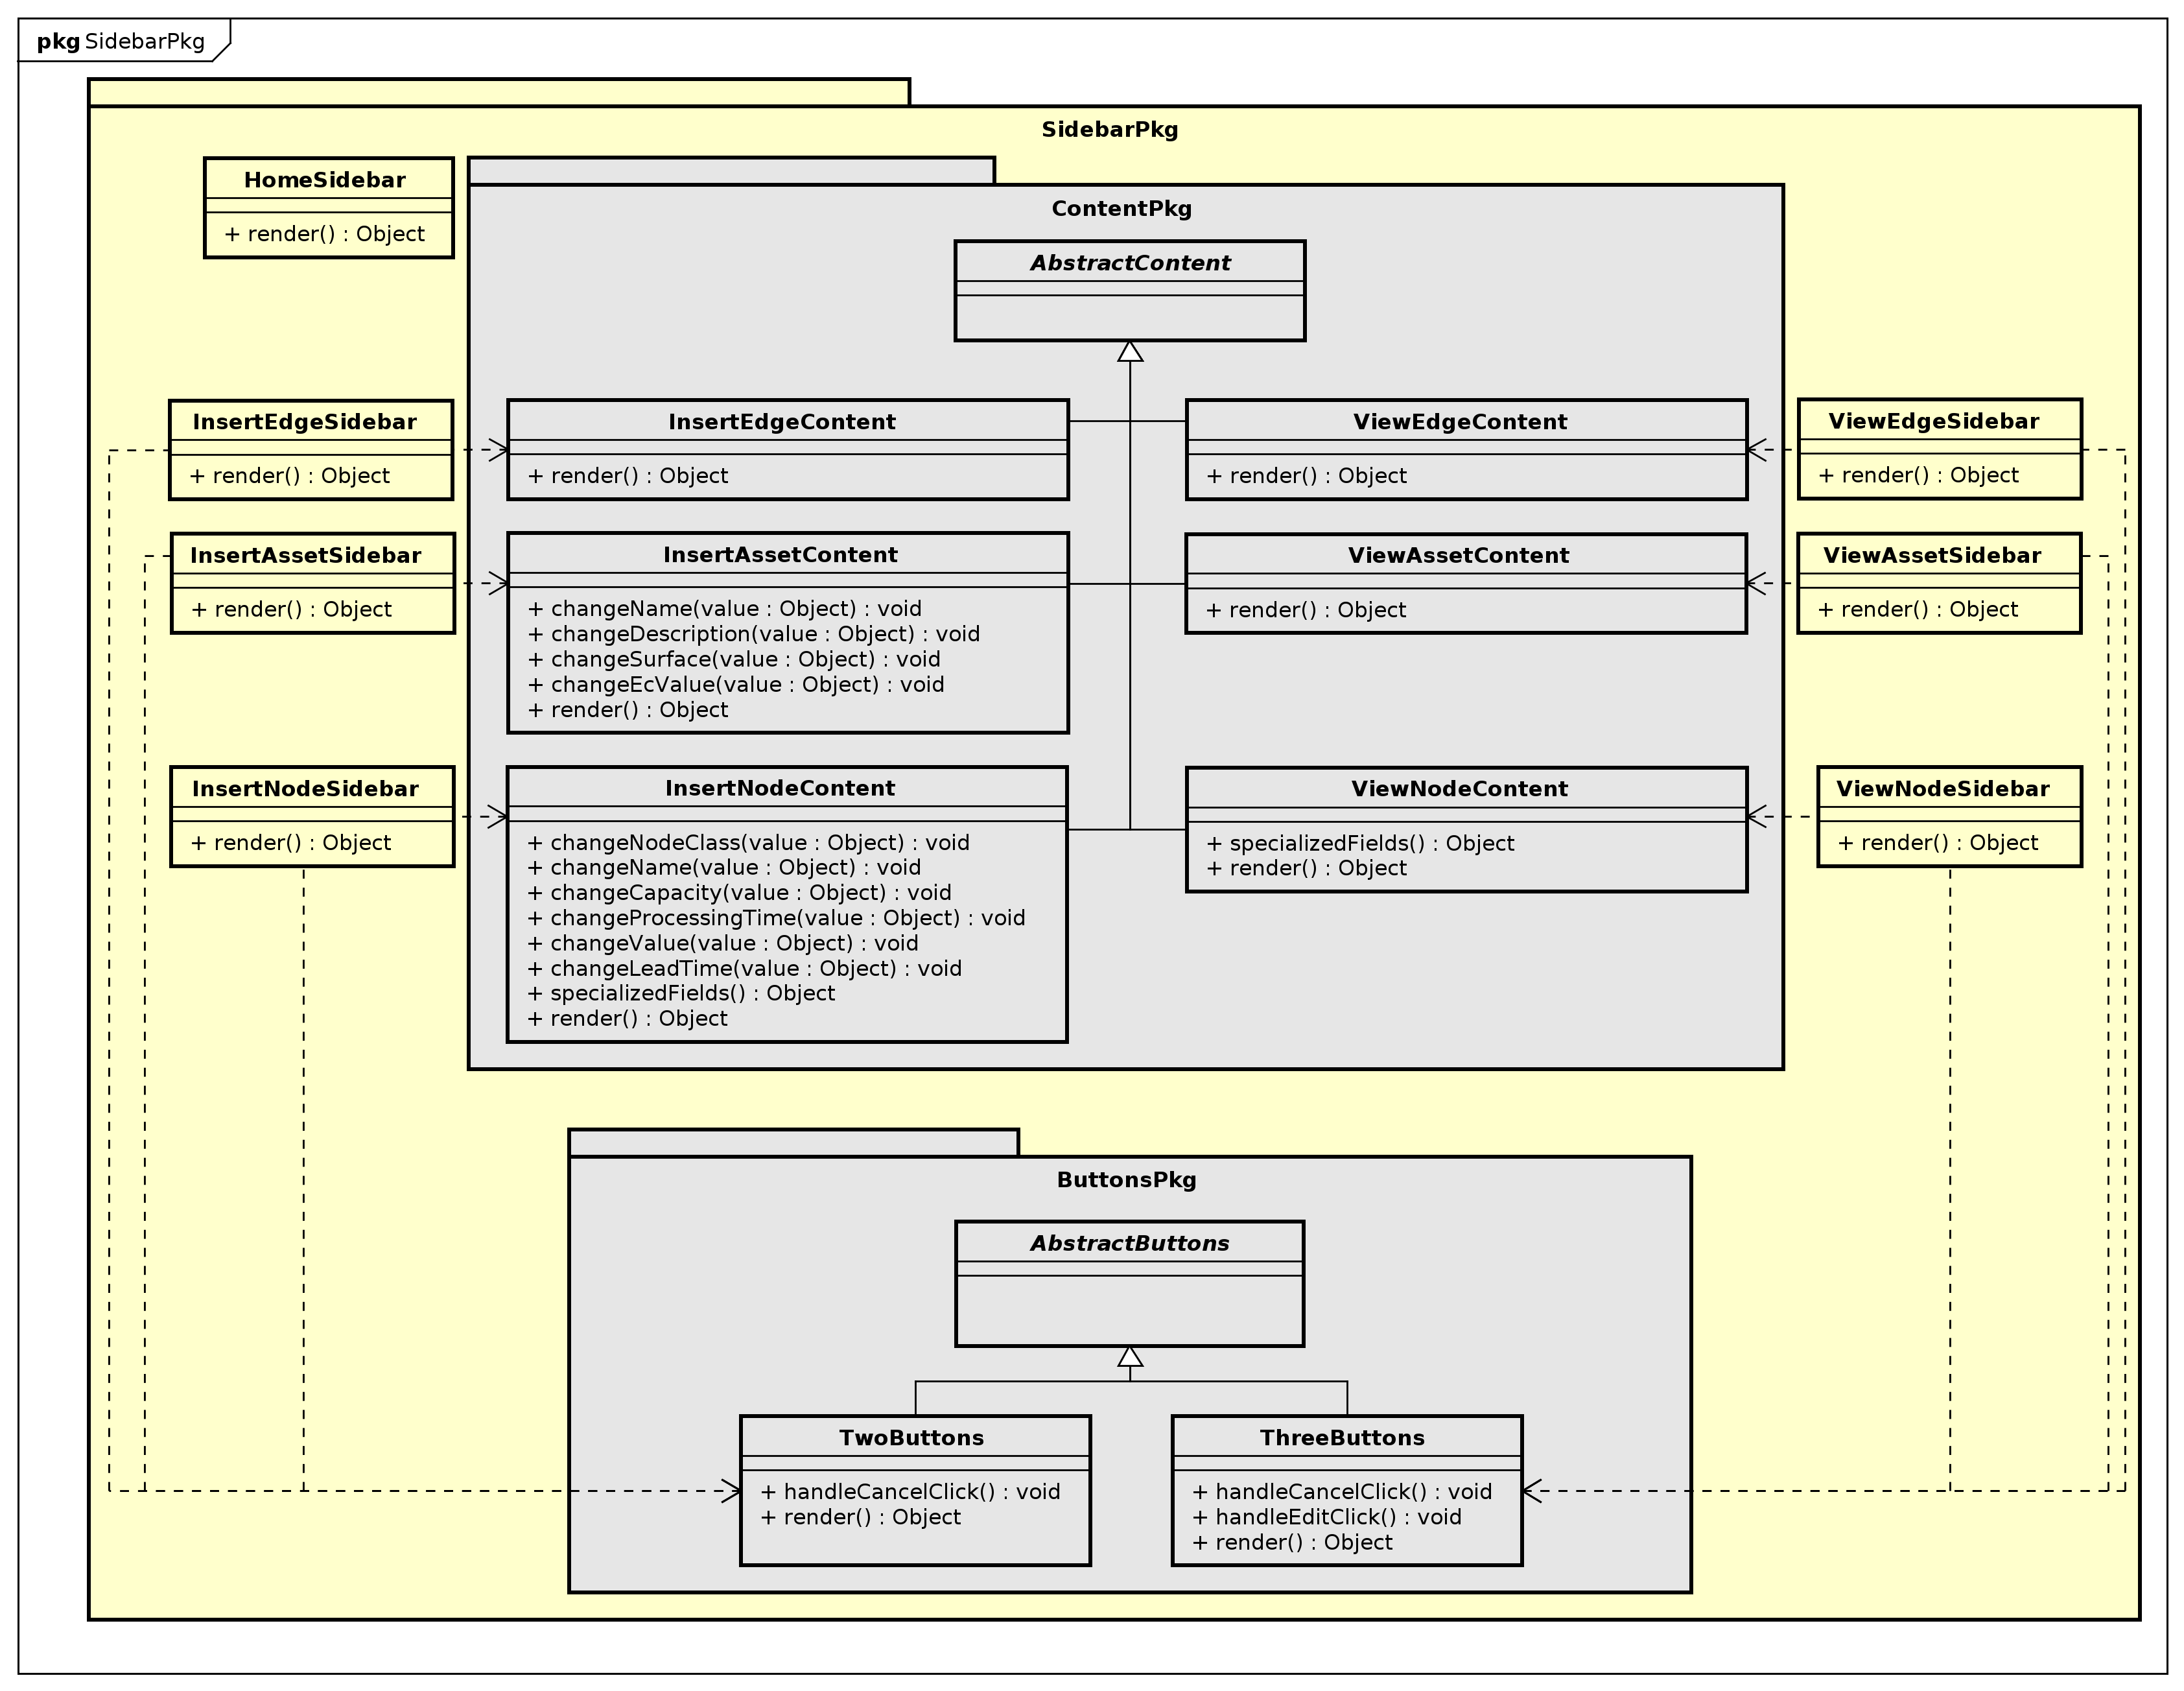
\includegraphics[width=\textwidth]{img/PkgDiagram/SidebarPkg.png}
	\caption{Schema componente DeGeOP::ViewPkg::SidebarPkg}
\end{figure}
\subsubsection{Informazioni sul package}
\begin{itemize}
	\item \textbf{descrizione:} racchiude le componenti necessarie alla rappresentazione della sidebar;
	\item \textbf{padre:} \hyperref[pkg::ViewPkg]{ViewPkg};
	\item \textbf{package contenuti:}
	\begin{itemize}
		\item SidebarPkg::\hyperref[pkg::ButtonsPkg]{ButtonsPkg};
		\item SidebarPkg::\hyperref[pkg::ContentPkg]{ContentPkg}.
	\end{itemize}
	\item \textbf{interazioni con altri package:} 
	\begin{itemize}
		\item IN DeGeOPViewPkg: utilizzo della sidebar.
	\end{itemize}
	\item \textbf{classi contenute:}
	\begin{itemize}
		\item HomeSidebar;
		\item InsertAssetSidebar;
		\item InsertEdgeSidebar;
		\item InsertNodeSidebar;
		\item ViewAssetSidebar;
		\item ViewEdgeSidebar;
		\item ViewNodeSidebar.
	\end{itemize}
\end{itemize}
\subsubsection{Classi}
\paragraph{HomeSidebar}
\begin{itemize}
	\begin{figure}[H]
		\centering
		\includegraphics[width=0.3\textwidth]{./img/HomeSidebar.png}
		\caption{Diagramma classe HomeSidebar}
	\end{figure}
	\item \textbf{descrizione:} rappresenta la sidebar di default ;
	\item \textbf{utilizzo:} renderizza una sidebar di default che dà il benvenuto all'utente;
	\item \textbf{metodi:}
	\begin{itemize}
		\item +render() : Object\newline
		il metodo renderizza la sidebar di benvenuto
	\end{itemize}
\end{itemize}
\paragraph{InsertAssetSidebar}
\begin{itemize}
	\begin{figure}[H]
		\centering
		\includegraphics[width=0.3\textwidth]{./img/InsertAssetSidebar.png}
		\caption{Diagramma classe InsertAssetSidebar}
	\end{figure}
	\item \textbf{descrizione:} rappresenta una sidebar per l'inserimento e la modifica di un asset;
	\item \textbf{utilizzo:} renderizza una sidebar composta da contenuto in cui l'utente può compilare i dati e da bottoni che permettono di eseguire inserimenti e modifiche relative ad un asset;
	\item \textbf{metodi:}
	\begin{itemize}
		\item +render() : Object\newline
		il metodo renderizza la sidebar di inserimento e modifica di un asset, composta da un InsertAssetContent e da un TwoButtons
	\end{itemize}
\end{itemize}
\paragraph{InsertEdgeSidebar}
\begin{itemize}
	\begin{figure}[H]
		\centering
		\includegraphics[width=0.3\textwidth]{./img/InsertEdgeSidebar.png}
		\caption{Diagramma classe InsertEdgeSidebar}
	\end{figure}
	\item \textbf{descrizione:} rappresenta una sidebar per l'inserimento e la modifica di un arco;
	\item \textbf{utilizzo:} renderizza una sidebar composta da contenuto in cui l'utente può compilare i dati e da bottoni che permettono di eseguire inserimenti e modifiche relative ad un arco;
	\item \textbf{metodi:}
	\begin{itemize}
		\item +render() : Object\newline
		il metodo renderizza la sidebar di inserimento e modifica di un arco, composta da un InsertEdgeContent e da un TwoButtons
	\end{itemize}
\end{itemize}
\paragraph{InsertNodeSidebar}
\begin{itemize}
	\begin{figure}[H]
		\centering
		\includegraphics[width=0.3\textwidth]{./img/InsertNodeSidebar.png}
		\caption{Diagramma classe InsertNodeSidebar}
	\end{figure}
	\item \textbf{descrizione:} rappresenta una sidebar per l'inserimento e la modifica di un nodo;
	\item \textbf{utilizzo:} renderizza una sidebar composta da contenuto in cui l'utente può compilare i dati e da bottoni che permettono di eseguire inserimenti e modifiche relative ad un nodo;
	\item \textbf{metodi:}
	\begin{itemize}
		\item +render() : Object\newline
		il metodo renderizza la sidebar di inserimento e modifica di un nodo, composta da un InsertNodeContent e da un TwoButtons
	\end{itemize}
\end{itemize}
\paragraph{ViewAssetSidebar}
\begin{itemize}
	\begin{figure}[H]
		\centering
		\includegraphics[width=0.3\textwidth]{./img/ViewAssetSidebar.png}
		\caption{Diagramma classe ViewAssetSidebar}
	\end{figure}
	\item \textbf{descrizione:} rappresenta una sidebar per la visualizzazione di un asset;
	\item \textbf{utilizzo:} renderizza una sidebar composta da contenuto in cui l'utente può visualizzare i dati e da bottoni che permettono di effettuare l'eliminazione dell'asset;
	\item \textbf{metodi:}
	\begin{itemize}
		\item +render() : Object\newline
		il metodo renderizza una sidebar per la visualizzazione di un asset, composta da un ViewAssetContent e da un ThreeButtons
	\end{itemize}
\end{itemize}
\paragraph{ViewEdgeSidebar}
\begin{itemize}
	\begin{figure}[H]
		\centering
		\includegraphics[width=0.3\textwidth]{./img/ViewEdgeSidebar.png}
		\caption{Diagramma classe ViewEdgeSidebar}
	\end{figure}
	\item \textbf{descrizione:} rappresenta una sidebar per l'inserimento e la modifica di un arco;
	\item \textbf{utilizzo:} renderizza una sidebar composta da contenuto in cui l'utente può visualizzare i dati e da bottoni che permettono di effettuare l'eliminazione dell'arco;
	\item \textbf{metodi:}
	\begin{itemize}
		\item +render() : Object\newline
		il metodo renderizza una sidebar per la visualizzazione di un arco, composta da un ViewEdgeContent e da un ThreeButtons
	\end{itemize}
\end{itemize}
\paragraph{ViewNodeSidebar}
\begin{itemize}
	\begin{figure}[H]
		\centering
		\includegraphics[width=0.3\textwidth]{./img/ViewNodeSidebar.png}
		\caption{Diagramma classe ViewNodeSidebar}
	\end{figure}
	\item \textbf{descrizione:} rappresenta una sidebar per la visualizzazione di un nodo;
	\item \textbf{utilizzo:} renderizza una sidebar composta da contenuto in cui l'utente può visualizzare i dati e da bottoni che permettono di effettuare l'eliminazione del nodo;
	\item \textbf{metodi:}
	\begin{itemize}
		\item +render() : Object\newline
		il metodo renderizza una sidebar per la visualizzazione di un arco, composta da un ViewNodeContent e da un ThreeButtons
	\end{itemize}
\end{itemize}
\newpage
\subsection{DeGeOP::ViewPkg::SidebarPkg::ContentPkg}
\label{pkg::ContentPkg}
\begin{figure}[H]
	\centering
	\includegraphics[width=\textwidth]{img/PkgDiagram/ContentPkg.png}
	\caption{Schema componente DeGeOP::ViewPkg::SidebarPkg::ContentPkg}
\end{figure}
\subsubsection{Informazioni sul package}
\begin{itemize}
	\item \textbf{descrizione:} racchiude le componenti che sono relative all'area informativa della Sidebar;
	\item \textbf{padre:} \hyperref[pkg::SidebarPkg]{SidebarPkg};
	\item \textbf{interazioni con altri package:} 
	\begin{itemize}
		\item IN FactorySidebarPkg: creazione contenuto della sidebar;
		\item OUT React-color: visualizzazione palette colori.
	\end{itemize}
	\item \textbf{classi contenute:}
	\begin{itemize}
		\item AbstractContent;
		\item InsertAssetContent;
		\item InsertEdgeContent;
		\item InsertNodeContent;
		\item ViewAssetContent;
		\item ViewEdgeContent;
		\item ViewNodeContent.
	\end{itemize}
\end{itemize}
\subsubsection{Classi}
\paragraph{AbstractContent}
\begin{itemize}
	\begin{figure}[H]
		\centering
		\includegraphics[width=0.3\textwidth]{./img/AbstractContent.png}
		\caption{Diagramma classe AbstractContent}
	\end{figure}
	\item \textbf{descrizione:} una classe d'interfaccia rappresentante il contenuto dell'area informativa nella sidebar;
	\item \textbf{utilizzo:} viene riferita da sidebar in quanto è una delle sue componenti.
\end{itemize}
\paragraph{InsertAssetContent}
\begin{itemize}
	\begin{figure}[H]
		\centering
		\includegraphics[width=0.3\textwidth]{./img/InsertAssetContent.png}
		\caption{Diagramma classe InsertAssetContent}
	\end{figure}
	\item \textbf{descrizione:} rappresenta il contenuto della sidebar relativa all'inserimento di un asset;
	\item \textbf{utilizzo:} viene creata da InsertAssetSidebarFactory ;
	\item \textbf{metodi:}
	\begin{itemize}
		\item +changeDescription() : void\newline
		delega il cambiamento dell'input della descrizione alla componente di livello più alto
		\item +changeEcValue(value) : void\newline
		delega il cambiamento dell'input del valore economico dell'asset alla componente di livello più alto
		\begin{itemize}
			\item value : string\\
			valore attualmente contenuto nell'input del valore economico dell'asset.
		\end{itemize}
		\item +changeName(value) : void\newline
		delega il cambiamento dell'input del nome dell'asset alla componente di livello più alto
		\begin{itemize}
			\item value : Object\\
			valore attualmente contenuto nell'input del nome dell'asset.
		\end{itemize}
		\item +changeSurface() : void\newline
		delega il cambiamento dell'input della superficie dell'asset alla componente di livello più alto
		\item +render() : Object\newline
		renderizza il contenuto della sidebar dell'asset in modalità inserimento e modifica
	\end{itemize}
\end{itemize}
\paragraph{InsertEdgeContent}
\begin{itemize}
	\begin{figure}[H]
		\centering
		\includegraphics[width=0.3\textwidth]{./img/InsertEdgeContent.png}
		\caption{Diagramma classe InsertEdgeContent}
	\end{figure}
	\item \textbf{descrizione:} rappresenta il contenuto della sidebar relativa all'inserimento di un arco;
	\item \textbf{utilizzo:} viene creata da InsertEdgeSidebarFactory ;
	\item \textbf{metodi:}
	\begin{itemize}
		\item +render() : Object\newline
		renderizza il contenuto della sidebar dell'arco in modalità inserimento e modifica
	\end{itemize}
\end{itemize}
\paragraph{InsertNodeContent}
\begin{itemize}
	\begin{figure}[H]
		\centering
		\includegraphics[width=0.3\textwidth]{./img/InsertNodeContent.png}
		\caption{Diagramma classe InsertNodeContent}
	\end{figure}
	\item \textbf{descrizione:} rappresenta il contenuto della sidebar relativa all'inserimento di un nodo;
	\item \textbf{utilizzo:} viene creata da InsertNodeSidebarFactory ;
	\item \textbf{metodi:}
	\begin{itemize}
		\item +changeCapacity() : void\newline
		delega il cambiamento della capacità del nodo alla componente di più alto livello
		\item +changeLeadTime(value) : void\newline
		delega il cambiamento del tempo di approvigionamento del nodo alla componente di più alto livello
		\begin{itemize}
			\item value : string\\
			valore che è contenuto nel dropdown della classe del nodo.
		\end{itemize}
		\item +changeName(value) : void\newline
		delega il cambiamento del nome del nodo alla componente di più alto livello
		\begin{itemize}
			\item value : string\\
			valore che è contenuto nel dropdown della classe del nodo.
		\end{itemize}
		\item +changeNodeClass(value) : void\newline
		delega il cambiamento del dropdown del nome del nodo alla componente di più alto livello
		\begin{itemize}
			\item value : string\\
			valore che è contenuto nel dropdown della classe del node.
		\end{itemize}
		\item +changeProcessingTime(value) : void\newline
		delega il cambiamento del valore del nodo alla componente di più alto livello
		\begin{itemize}
			\item value : string\\
			valore che è contenuto nel dropdown della classe del nodo.
		\end{itemize}
		\item +render() : Object\newline
		renderizza il il contenuto della sidebar del node in modalità inserimento e modifica
		\item +specializedFields() : Object\newline
		metodo che gestisce i campi dati da visualizzare a seconda della tipologia del nodo
	\end{itemize}
\end{itemize}
\paragraph{ViewAssetContent}
\begin{itemize}
	\begin{figure}[H]
		\centering
		\includegraphics[width=0.3\textwidth]{./img/ViewAssetContent.png}
		\caption{Diagramma classe ViewAssetContent}
	\end{figure}
	\item \textbf{descrizione:} rappresenta il contenuto della sidebar relativa alla visualizzazione di un asset;
	\item \textbf{utilizzo:} viene creata da ViewAssetSidebarFactory ;
	\item \textbf{metodi:}
	\begin{itemize}
		\item +render() : Object\newline
		renderizza la parte di sidebar relativa alla visualizzazione dei campi dati di un asset
	\end{itemize}
\end{itemize}
\paragraph{ViewEdgeContent}
\begin{itemize}
	\begin{figure}[H]
		\centering
		\includegraphics[width=0.3\textwidth]{./img/ViewEdgeContent.png}
		\caption{Diagramma classe ViewEdgeContent}
	\end{figure}
	\item \textbf{descrizione:} rappresenta il contenuto della sidebar relativa alla visualizzazione di un arco;
	\item \textbf{utilizzo:} viene creata da ViewEdgeSidebarFactory ;
	\item \textbf{metodi:}
	\begin{itemize}
		\item +render() : Object\newline
		renderizza la parte di sidebar relativa alla visualizzazione dei campi dati di un arco
		\item +specializedFields() : Object\newline
		si occupa della visualizzazione dei campi dati a seconda della tipologia del nodo
	\end{itemize}
\end{itemize}
\paragraph{ViewNodeContent}
\begin{itemize}
	\begin{figure}[H]
		\centering
		\includegraphics[width=0.3\textwidth]{./img/ViewNodeContent.png}
		\caption{Diagramma classe ViewNodeContent}
	\end{figure}
	\item \textbf{descrizione:} rappresenta il contenuto della sidebar relativa alla visualizzazione di un ndo;
	\item \textbf{utilizzo:} viene creata da ViewNodeSidebarFactory ;
	\item \textbf{metodi:}
	\begin{itemize}
		\item +render() : Object\newline
		renderizza la parte di sidebar relativa alla visualizzazione dei campi dati di un nodo
	\end{itemize}
\end{itemize}
\newpage
\subsection{DeGeOP::ViewPkg::SidebarPkg::ButtonsPkg}
\label{pkg::ButtonsPkg}
\begin{figure}[H]
	\centering
	\includegraphics[width=\textwidth]{img/PkgDiagram/ButtonsPkg.png}
	\caption{Schema componente DeGeOP::ViewPkg::SidebarPkg::ButtonsPkg}
\end{figure}
\subsubsection{Informazioni sul package}
\begin{itemize}
	\item \textbf{descrizione:} racchiude le componenti che sono relative all'area con i bottoni della Sidebar;
	\item \textbf{padre:} \hyperref[pkg::SidebarPkg]{SidebarPkg};
	\item \textbf{classi contenute:}
	\begin{itemize}
		\item AbstractButtons;
		\item ThreeButtons;
		\item TwoButtons.
	\end{itemize}
\end{itemize}
\subsubsection{Classi}
\paragraph{AbstractButtons}
\begin{itemize}
	\begin{figure}[H]
		\centering
		\includegraphics[width=0.3\textwidth]{./img/AbstractButtons.png}
		\caption{Diagramma classe AbstractButtons}
	\end{figure}
	\item \textbf{descrizione:} una classe d'interfaccia rappresentante i bottoni inseriti nella sidebar;
	\item \textbf{utilizzo:} viene riferita da sidebar in quanto è una delle sue componenti.
\end{itemize}
\paragraph{ThreeButtons}
\begin{itemize}
	\begin{figure}[H]
		\centering
		\includegraphics[width=0.3\textwidth]{./img/ThreeButtons.png}
		\caption{Diagramma classe ThreeButtons}
	\end{figure}
	\item \textbf{descrizione:} classe che renderizza tre bottoni, uno di modifica,  uno di eliminazione e uno di annullamento. Il bottone di annullamento provoca l'annullamento della selezione corrente. Il bottone di eliminazione provoca la comparsa di una finestra modale che chiede la conferma dell'eliminazione dell'elemento correntemente selezionato. Il bottone di modifica provoca l'avvio della modalità di modifica, con cui è possibile ridisegnare l'asset o cambiare i campi dati;
	\item \textbf{utilizzo:} viene utilizzata nelle sidebar di visualizzazione;
	\item \textbf{metodi:}
	\begin{itemize}
		\item +handleCancelClick() : void\newline
		il metodo gestisce il click sul bottone di annullamento, ripristinando la sidebar di default
		\item +handleEditClick() : void\newline
		il metodo imposta la sidebar di modifica dell'elemento attualmente selezionato
		\item +render() : Object\newline
		renderizza tre bottoni, uno di modifica, uno di annullamento e uno di eliminazione
	\end{itemize}
\end{itemize}
\paragraph{TwoButtons}
\begin{itemize}
	\begin{figure}[H]
		\centering
		\includegraphics[width=0.3\textwidth]{./img/TwoButtons.png}
		\caption{Diagramma classe TwoButtons}
	\end{figure}
	\item \textbf{descrizione:} classe che renderizza due bottoni, uno di salvataggio e uno di annullamento. Il bottone di salvataggio è disabilitato fino a che tutti i campi della sidebar non sono stati compilati in modo corretto. Il bottone di annullamento provoca l'interruzione dell'inserimento dei dati;
	\item \textbf{utilizzo:} viene utilizzata nelle sidebar di inserimento;
	\item \textbf{metodi:}
	\begin{itemize}
		\item +handleCancelClick() : void\newline
		il metodo gestisce il click sul bottone di annullamento, ripristinando la sidebar di default
		\item +render() : Object\newline
		renderizza due bottoni, uno di annullamento e uno di salvataggio
	\end{itemize}
\end{itemize}
\newpage

\newpage

\section{Estensione delle funzionalità}
Per ragioni di tempo e competenze alcune funzionalità non sono state implementate. Inoltre lo sviluppo è stato guidato dall'architettura preesistente di \riskapp{} e dalle API disponibili al momento della presa in consegna del progetto \progetto.

\subsection{Scenari di danno}
Le funzionalità di aggiunta, visualizzazione, modifica ed eliminazione degli scenari di danno non sono state implementate. Le operazioni da svolgere per implementarle sono:
\begin{itemize}
	\item ottenere le API da \riskapp{} per interfacciarsi con il loro server;
	\item inserire in \textit{StorePkg} le classi necessarie all'implementazione della parte di Store relativa agli scenari, come descritto dal documento di \textit{Specifica Tecnica};
	\item inserire in \textit{ActionsPkg} le classi necessarie all'implementazione delle actions che operano sugli scenari, come descritto dal documento di \textit{Specifica Tecnica};
	\item inserire in \textit{ReducerPkg} le funzioni necessarie all'implementazione dei reducer che operano sugli scenari, come descritto dal documento di \textit{Specifica Tecnica};
	\item inserire in \textit{ViewPkg} le componenti React necessarie all'aggiunta, visualizzazione, modifica ed eliminazione degli scenari di danno, come descritto dal documento di \textit{Specifica Tecnica}.
	\item inserire in \textit{CallManagerPkg} le classi necessarie all'interfacciamento con il server \riskapp{}
	I campi dati relativi agli Scenari di danno, essendo informazioni di dettaglio, non sono riportati nella \textit{Specifica Tecnica}, ma sono ricavabili dal documento di \adr{}.
	Un buon esempio di come potrebbero essere implementati dal punto di vista dell'utente finale è descritto dal documento di \textit{Specifica Tecnica} nella sezione \textit{Attività}.
\end{itemize}

\subsection{Analisi di rischio}
La funzionalità di avvio ed eliminazione delle analisi di rischio non sono state implementate. Le operazioni da svolgere per implementarle sono:
\begin{itemize}
	\item ottenere le API da \riskapp{} per interfacciarsi con il loro server;
	\item inserire in \textit{StorePkg} le classi necessarie all'implementazione della parte di Store relativa alle analisi di rischio, come descritto dal documento di \textit{Specifica Tecnica};
	\item inserire in \textit{ActionsPkg} le classi necessarie all'implementazione delle actions che operano sulle analisi di rischio, come descritto dal documento di \textit{Specifica Tecnica};
	\item inserire in \textit{ReducerPkg} le funzioni necessarie all'implementazione dei reducer che operano sulle analisi di rischio, come descritto dal documento di \textit{Specifica Tecnica};
	\item inserire in \textit{ViewPkg} le componenti React necessarie all'avvio ed all'eliminazione delle analisi di rischio, come descritto dal documento di \textit{Specifica Tecnica}.
	\item inserire in \textit{CallManagerPkg} le classi necessarie all'interfacciamento con il server \riskapp{}.
	Un buon esempio di come potrebbero essere implementate dal punto di vista dell'utente finale è descritto dal documento di \textit{Specifica Tecnica} nella sezione \textit{Attività}.
\end{itemize}

\subsection{Nuova tipologia di nodo}
I nodi possono essere di diverse tipologie. In caso si volesse inserire una nuova tipologia di nodo, le operazioni da svolgere per implementarli sono:
\begin{itemize}
	\item ottenere le API da \riskapp{} per interfacciarsi con il loro server;
	\item inserire in \textit{StorePkg} la classe necessaria all'implementazione della parte di Store relativa a quel nodo. Questa classe deve estendere la classe \textit{Node};
	\item inserire in \textit{ActionsPkg} le classi necessarie all'implementazione delle actions che operano su quel nuovo tipo di nodo;
	\item inserire in \textit{ReducerPkg} le funzioni necessarie all'implementazione dei reducer che operano su quel nuovo tipo di nodo;
	\item inserire in \textit{ViewPkg} le componenti React necessarie all'avvio ed all'eliminazione delle analisi di rischio. In particolare nelle classi \textit{ViewPkg}::\textit{SidebarPkg}::\textit{ContentPkg}::\textit{InsertNodeContent} e \textit{ViewPkg}::\textit{SidebarPkg}::\textit{ContentPkg}::\textit{ViewNodeContent}, nella funzione \textit{specializedField()} che si occupa della renderizzazione dei campi dati specifici, aggiungere la sezione che renderizza i campi dati della nuova tipologia di nodo;
	\item inserire in \textit{CallManagerPkg} le classi necessarie all'interfacciamento con il server \riskapp{}.
\end{itemize}

%\medskip
%\begin{lstlisting}[caption=My Javascript Example]
%Name.prototype = {
%methodName: function(params){
%	var doubleQuoteString = "some text";
%	var singleQuoteString = 'some more text';
%	// this is a comment
%			if(this.confirmed != null && typeof(this.confirmed) == Boolean && this.confirmed == true){
%		document.createElement('h3');
%		$('#system').append("This looks great");
%		return false;
%} else {
%	throw new Error;
%}
%}
%}
%\end{lstlisting}

%Le principali funzionalità:
%multi processo
%api 
%portare le loro funzionalita in single page
%visualizzazione degli scenari e i risulatati dell'analisi su quegli scenari
%	gradiente
%	hazard
%report/statistiche -> print
%stampare schema del processo (quindi altre visualizzazioni)
%(mappa satellitare)
\newpage

\section{Estensione del codice}

\subsection{Creazione di una nuova categoria di sidebar}
Le sidebar presentano, come richiesto da React una struttura altamente modulare.
Per aggiungere una nuova sidebar di seguito denominata per comodità \textit{NewSidebar} si devono effettuare le seguenti operazioni:
\begin{itemize}
	\item aggiungere \textit{ViewPkg}::\textit{DeGeOPView}::\textit{DeGeOPView}, nella funzione \textit{sidebarFactory()} il \textit{conditional render} della nuova sidebar;
	\item aggiungere in \textit{ViewPkg}::\textit{DeGeOPView} la componente React  \textit{NewSidebar} che renderizza la sidebar. Essendo ogni sidebar divisa in due sezioni (contenuto e bottoni), per renderizzarla dovranno venire a sua volta richiamate le renderizzazioni:
	\begin{itemize}
		\item della nuova componente React (da creare anch'essa) \textit{ViewPkg}::\textit{DeGeOPView}::\textit{ContentPkg}::\textit{NewSidebarContent};
		\item di una delle componenti a scelta tra \textit{ViewPkg}::\textit{DeGeOPView}::\textit{ButtonsPkg}::\textit{threeButtons}, \textit{ViewPkg}::\textit{DeGeOPView}::\textit{ButtonsPkg}::\textit{twoButtons}.
	\end{itemize}
\end{itemize}

\subsection{Aggiornamenti dei campi dati di asset e nodi}
Visto che \riskapp{} utilizza il modello di sviluppo Agile, il loro server e i file JSON che esso ritorna, sono soggetti a continui e rapidi cambiamenti. Di seguito viene descritto come estendere il codice in caso venissero aggiunti nuovi campi dati per asset o nodi.

\subsubsection{Asset}In caso venissero aggiunti nuovi campi dati per un asset seguire i seguenti passi:
\begin{itemize}
	\item aggiungere in \textit{StorePkg}::\textit{ProcessPkg}::\textit{Asset} il campo dati e le funzioni per gestire le sue eventuali validazioni;
	\item aggiungere nello \textit{state} \textit{ViewPkg}::\textit{DeGeOPView}::\textit{DeGeOPView} il campo dati e le sue validazioni e in		\textit{ViewPkg}::\textit{SidebarPkg}::\textit{ContentPkg}::\textit{InsertAssetContent} e \textit{ViewPkg}::\textit{SidebarPkg}::\textit{ContentPkg}::\textit{ViewAssetContent} aggiungere il campo dati di interesse utilizzando le componenti di React-Toolbox, come descritto nella \textit{Specifica Tecnica}.
\end{itemize}

\subsubsection{Nodo}In caso venissero aggiunti nuovi campi dati per un  nodo seguire i seguenti passi:
\begin{itemize}
	\item aggiungere in \textit{StorePkg}::\textit{ProcessPkg}::\textit{Node} nelle sue derivate il campo dati e le funzioni per gestire le sue eventuali validazioni;
	\item aggiungere nello \textit{state} \textit{ViewPkg}::\textit{DeGeOPView}::\textit{DeGeOPView} il campo dati e le sue validazioni e in		\textit{ViewPkg}::\textit{SidebarPkg}::\textit{ContentPkg}::\textit{InsertNodeContent} e \textit{ViewPkg}::\textit{SidebarPkg}::\textit{ContentPkg}::\textit{ViewNodeContent} aggiungere il campo dati di interesse utilizzando le componenti di React-Toolbox, come descritto nella \textit{Specifica Tecnica}.
\end{itemize}

%Se cambiano le API -> aggiungere campi dati agli asset, nodi, archi
%supporto al multilingua
%nuovo tipo di nodo
%aggiungere foto all'asset (campi dati)
%nuovi tipi di azioni operabili sul modello (Reducer->nuovo blocco)
%sile css inline + react-toolbox-themr per modificare la presentazione dei componenti toolbox
%gestore chiamate???
%marker nodi 
%react-dev tools
%redux-dev tools 
%nel sisstema di build + nel chrome store -> sisitea di build in sistema di development
%aiuto per trovare bug

\appendix
\section{Glossario}
	\subsection{A}
	
		\mgref{Action}
		In Redux, oggetto che descrive un cambiamento di stato.
		
		\mgref{API}
		\textit{Application Programming Interface}. Insieme di procedure utilizzabili per interfacciarsi con un programma o un sistema informatico in modo standard. Spesso si intendono le librerie software disponibili in un certo linguaggio di programmazione.
	
		\mgref{Arco}
		Collegamento orientato tra due nodi.
		
		\mgref{Asset}
		Fabbricato con importanza strategica per il processo produttivo di un'azienda. Un asset può contenere uno o più nodi.
		
		\mgref{Asus}
		Azienda produttrice di dispositivi tecnologici di varia tipologia.
		
	\subsection{B}

		\mgref{Browser}
		Il web browser, o più semplicemente browser, è un'applicazione per il recupero, la presentazione e la navigazione di risorse web. Tali risorse (ad esempio pagine web, immagini, video) sono a disposizione sul World Wide Web su una rete locale o sullo stesso computer dove il browser è in esecuzione.
		
	\subsection{C}
		\mgref{Chrome}		
		\mglo{Browser}{Browser} web sviluppato da Google.
		
		\mgref{Componente}
		\begin{enumerate}
			\item React: elemento che fa parte della gerarchia del DOM. L'elemento eredita dalla classe base astratta React.Component.
			\item Unità software dotata di una precisa identità e interfacce ben definite.
		\end{enumerate}
		
		\mgref{Cross-platform}
		Possibilità di poter usare lo stesso strumento software su diversi sistemi operativi.
		
		\mgref{CSS}
		\textit{Cascading Style Sheets}. Linguaggio che permette di definire lo stile e la formattazione di una pagina \glo{HTML}{HTML}. Permette di mantenere separate presentazione e contenuto. \\
		La versione stabile più recente è CSS3.
		
	\subsection{D}
	
	\mgref{Design pattern}
	Soluzione progettuale generale per la risoluzione di un problema ricorrente. \\
	I design pattern orientati agli oggetti tipicamente mostrano relazioni ed interazioni tra classi o oggetti.
	Ad un livello più alto si trovano invece i pattern architetturali, con ambito più ampio. Essi descrivono un pattern complessivo adottato dall'intero sistema.
	
	\mgref{Dispatch}
	In Redux, metodo per inviare un'azione allo store.
	
	\mgref{DOM}
	\textit{Document Object Model}. Forma di rappresentazione dei documenti strutturati come modello orientato agli oggetti, definita dal \mglo{W3C}{W3C}.
	
	\subsection{E}
	
	\mgref{ESLint}
	Tool per l'analisi statica del codice \mglo{JavaScript}{JavaScript}.
	
	\subsection{F}
		\mgref{Firefox}
		\mglo{Browser}{Browser} web  libero e multipiattaforma, mantenuto da Mozilla Foundation.
		
		\mgref{Framework}
		Insieme di classi cooperanti che forniscono lo scheletro di un'applicazione riusabile per uno specifico dominio applicativo. Delinea l'architettura delle applicazioni in cui viene usato.
		
	\subsection{G}
		\mgref{Gesture}
		Combinazione di movimenti e click del dispositivo di puntamento (ad esempio il mouse) che vengono riconosciuti come comandi specifici.
		
		\mgref{Git}
		\mglo{Sistema di controllo di versione}{Sistema di controllo di versione} distribuito e \mglo{Open source}{open source}, creato da Linus Torvalds nel 2005.
		Vari progetti software usano Git per il controllo del versionamento, principalmente il kernel \mglo{Linux}{Linux}.
		
		\mgref{GitHub}
		Servizio Web per il controllo di versione basato su \mglo{Git}{Git}. Offre diversi piani per \mglo{Repository}{repository} privati sia a pagamento che gratuiti, molto utilizzati per lo sviluppo di progetti \mglo{Open source}{open source}.
		
		\mgref{Gruppo}
		Componenti che fanno parte del gruppo \zephyrus.
	\subsection{H}
	
	\mgref{HTML}
	\textit{HyperText Markup Language}. Linguaggio usato per la definizione di pagine Web; la sua sintassi è stabilita dal \mglo{W3C}{W3C}.
	HTML5 è l'ultima versione stabile.
	
	\subsection{I}
		\mgref{IDE}
		\textit{Integrated Development Enviroment}. Software utilizzato per la scrittura di codice sorgente. Spesso aiuta il programmatore segnalando errori di sintassi, oltre a tutta una serie di strumenti e funzionalità di supporto allo sviluppo.
	
		\mgref{iOS}
		Sistema operativo sviluppato da Apple Inc.
	
		\mgref{Ipad}
		Tablet prodotto dall'azienda Apple Inc.
	\subsection{J}
	
	\mgref{JavaScript}
	Linguaggio di scripting orientato agli oggetti e agli eventi. È utilizzato prevalentemente nella programmazione Web lato client per la creazione di effetti dinamici interattivi.
	
%	\subsection{K}
	\subsection{L}
	
		\mgref{Libreria}
		Insieme di funzioni e strutture dati predefinite e predisposte per lo sviluppo di software.
		
		\mgref{Linguaggio di markup}
		Insieme di regole che descrivono i meccanismi di rappresentazione (strutturali, semantici o presentazionali) di un testo che, utilizzando convenzioni standardizzate, sono utilizzabili su più supporti.
		
		\mgref{Linux}
		Linux è una famiglia di sistemi operativi di tipo Unix-like, rilasciati sotto varie distribuzioni, aventi la caratteristica comune di utilizzare come nucleo il kernel Linux. Ubuntu è la distribuzione di Linux più utilizzata.
	\subsection{M}
		\mgref{MacOS}
		Sistema operativo sviluppato da Apple.
	\subsection{N}
		\mgref{Node.js}
		Runtime \mglo{JavaScript}{JavaScript} costruito sul motore V8 di Chrome.
	
		\mgref{Nodo}
		Oggetto che fa parte dei processo produttivo aziendale. È contenuto all'interno di un asset.
	\subsection{O}
		\mgref{Open source}
		Software di cui i detentori dei diritti rendono pubblico il codice sorgente, permettendo ad altri programmatori di apportarvi modifiche. Questa possibilità è regolata tramite l’applicazione di apposite licenze d’uso.
		
		\mgref{OpenStreetMap}
		Servizio di mappe liberamente modificabili dell'intero pianeta.
	
	\subsection{P}
	
	\mgref{Package}
	Costrutto per organizzare classi logicamente correlate o che forniscono servizi simili, all'interno di sottogruppi ordinati. I package possono essere compressi permettendo la trasmissione di più classi in una sola volta. In \mglo{UML}{UML}, analogamente, è un raggruppamento arbitrario di elementi in una unità di livello più alto.
		
	\mgref{Proprietà}
	Input con i quali sono costruite le componenti React.
	
%	\subsection{Q}
	\subsection{R}
	
		\mgref{React}
		Libreria \mglo{JavaScript}{JavaScript} per la creazione di interfacce grafiche.
		
		\mgref{Reducer}
		In Redux, funzione che restituisce un nuovo stato dello store in seguito ad un'azione.
		
		\mgref{Render}
		Metodo richiesto da React.Component per la visualizzazione delle componenti sul DOM virtuale.
		
		\mgref{Repository}
		Ambiente di un sistema informativo in cui vengono gestiti i metadati attraverso
		tabelle relazionali. Il repository utilizzato dal \mglo{Gruppo}{gruppo} \zephyrus{} è fornito
		dalla piattaforma \mglo{GitHub}{GitHub}.
		
		\mgref{REST}
		Stile architetturale che offre la possibilità di manipolare rappresentazioni testuali di risorse Web utilizzando un set predefinito di operazioni.
	
	\subsection{S}
	
		\mgref{Safari}
		\mglo{Browser}{browser} web sviluppato dalla Apple.
		
		\mgref{Sistema di controllo di versione}
		Strumento che consente di tracciare le modifiche a cui viene sottoposto un insieme di file, consentendo di accedere alle vecchie versioni e di lavorare in più persone contemporaneamente.
		
		\mgref{Store}
		In Redux, ilcontenitore degli stati dell'applicazione.
		
%	\subsection{T}
%	\subsection{U}
	\subsection{V}
		\mgref{VirtualBox}
		Software open source per l'esecuzione di macchine virtuali.
	\subsection{W}
	
		\mgref{W3C}
		\textit{World Wide Web Consortium}. Organizzazione non governativa internazionale che ha come scopo quello di sviluppare tutte le potenzialità del World Wide Web. Al fine di riuscire nel proprio intento, la principale attività svolta dal W3C consiste nello stabilire standard tecnici che riguardino sia i linguaggi di markup che i protocolli di comunicazione.
		
		\mgref{WebStorm}
		\mglo{IDE}{IDE} che offre supporto allo sviluppo di applicazioni \mglo{JavaScript}{JavaScript} sia client che server. Offre inoltre supporto a \mglo{Node.js}{Node.JS}, \mglo{HTML}{HTML}, \mglo{CSS}{CSS} e frameworks come AngularJS e a librerie JavaScript come React.
		
		\mgref{Windows}
		Sistema operativo sviluppato da Microsoft.
%	\subsection{X}
%	\subsection{Y}
%	\subsection{Z}
\end{document}

%ATTENZIONE concentrarsi maggiormente su esempi concreti di manutenzione, assumendo (e richiedendo) che lo sviluppatore conosca già le tecnologie che dovrà utilizzare.

%AAA Manca completamente un Glossario dedicato.
%AAA Qual è l’URL al quale collegarsi per accedere al sistema? 
%AAA Non è descritto il processo di segnalazione di eventuali errori del prodotto. Il documento è completamente privo di immagini che aiutino l’utente a collegare le descrizioni presenti al prodotto vero e proprio.

%TODO 1) Evidenziare le tecnologie utillzate,
%TODO 2) Strumenti necessari
%TODO 3) Glossario Dedicato
%TODO Estensione funzionalità
%TODO Estensione del codice